\documentclass[12pt,UTF8]{ctexbook}
\usepackage{multirow}
\usepackage{booktabs}
% 导入设定
\input{../shared/settings}

% 封面
\title{\zihao{0} \bfseries 第四册}
\author{\zihao{2} \texttt{大青花鱼}}
% \date{\bfseries\today}
\date{}
% 正文
\begin{document}
\maketitle
\tableofcontents
\newpage

\chapter{四边形}
四边形是生活中常见的形状。下面来看几种常见的四边形。
\section{平行四边形}

\textbf{平行四边形}是一种重要的四边形。它由两组平行线确定。

设直线$l_1 \parallel l_2$，$m_1 \parallel m_2$，且$l_1$和$m_1$有交点$A$，
那么$l_2$和$m_1$、$l_2$和$m_2$、$l_1$和$m_2$各有交点$B$、$C$、$D$，四边形$ABCD$
叫做平行四边形，记作$\parasbx ABCD$。

\begin{wrapfigure}[7]{r}{0.3\textwidth} %this figure will be at the right
    \vspace{-24pt}
    \centering
    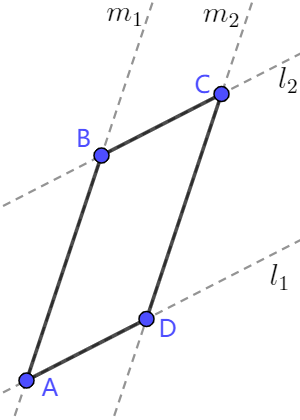
\includegraphics[width=0.3\textwidth]{tu/平行四边形0.png}
\end{wrapfigure}

设有四边形$ABCD$，我们说$AB$、$CD$互为\textbf{对边}，$BC$、$DA$互为对边；
$\angle ABC$和$\angle CDA$互为\textbf{对角}，$\angle BCD$和$\angle DAB$互为对角。
线段$AC$和$BD$称为四边形的\textbf{对角线}。

\begin{tm}\label{tm:0-0-0}
    平行四边形对边平行且等长，对角相等。
\end{tm}
\begin{proof}
    给定$\parasbx ABCD$，按定义可知对边平行。\\
    接着证明$\parasbx ABCD$的对角相等。\\
    $\angle ABC$和$\angle DAB$是同旁内角，所以和为平角。类似地，$\angle ABC$和$\angle BCD$是同旁内角，所以和为平角。于是，$\angle DAB = \angle BCD$。同理， $\angle ABC$和$\angle DAB$是同旁内角，所以和为平角。类似地，$\angle CDA$和$\angle DAB$是同旁内角，所以和为平角。于是，$\angle ABC = \angle CDA$。\\
    最后证明$\parasbx ABCD$的对边等长。\\
    连接对角线$AC$。$AB \parallel CD$，所以内错角$\angle CAB = \angle ACD$；同理，$BC \parallel DA$，所以内错角$\angle BCA = \angle DAC$。另外$|AC| = |AC|$。所以，根据“角边角”，$\triangle ABC \simeq \triangle CDA$。因此，$|AB| = |CD|$，$|BC| = |DA|$。    
\end{proof}

从证明中可以看出，平行四边形和三角形有密切的关系。把平行四边形沿对角线“裁开”，就得到一对同角全等的三角形。
一般来说，任何四边形沿对角线裁开，都会得到两个三角形。
因此，在约定角的范围是负平角到正平角时，\textbf{四边形的内角和是零角}。
对平行四边形来说，为了方便，也说它的内角和是周角。

除了对边分别平行，还有什么办法，判断一个四边形是不是平行四边形呢？
我们可以从这对全等三角形入手。以上证明中用到了“角边角”，是否可以换成“边角边”或“边边边”呢？

\begin{tm}\label{tm:0-0-1}
    对边等长的四边形是平行四边形。
\end{tm}
\begin{proof}
    设四边形$ABCD$中$|AB| = |CD|$，$|BC| = |DA|$。连接$AC$，根据“边边边”，
    $\triangle ABC \simeq \triangle CDA$，因此，$\angle CAB = \angle ACD$，
    于是$AB \parallel CD$。同理，由于$\angle BCA = \angle DAC$，$BC \parallel DA$。
    于是四边形$ABCD$是平行四边形。
\end{proof}

\begin{tm}\label{tm:0-0-2}
    一对边平行且等长的四边形是平行四边形。
\end{tm}
\begin{proof}
    设四边形$ABCD$中$AB \parallel CD$且$|AB| = |CD|$。连接$AC$。
    $|AC| = |AC|$。由于$AB \parallel CD$，内错角$\angle CAB = \angle ACD$。
    根据“边角边”，$\triangle ABC \simeq \triangle CDA$，因此，
    由于$\angle BCA = \angle DAC$，$BC \parallel DA$。于是四边形$ABCD$是平行四边形。
\end{proof}

\begin{tm}\label{tm:0-0-3}
    对角相等的四边形是平行四边形。
\end{tm}
\begin{proof}
    设四边形$ABCD$中$\angle ABC = \angle CDA$，$\angle BCD = \angle DAB$。
    四边形的内角和是两个平角，所以同旁内角$\angle ABC$和$\angle BCD$满足
    $\angle ABC + \angle BCD = 180^\circ$，这说明$AB \parallel CD$。
    同理，同旁内角$\angle ABC$和$\angle DAB$满足$\angle ABC + \angle DAB = 180^\circ$，
    因此$BC \parallel DA$。
\end{proof}

\begin{sk}\label{sk:0-0-0}
    一对边等长，一对角相等的四边形，是否是平行四边形？
\end{sk}

给定$\parasbx ABCD$，设对角线$AC$和$BD$的交点为$G$，我们把$G$叫做平行四边形的\textbf{中心}。
可以用“角边角”证明：$\triangle ABG \simeq \triangle CDG$，$\triangle BCG \simeq \triangle DAG$。
因此，$|AG| = |CG|$、$|BG| = |DG|$。$G$同时是两条对角线的中点。
换句话说，\textbf{平行四边形的两条对角线相互平分}。
用对称的说法，$A$和$C$关于$G$对称，$B$和$D$关于$G$对称。

在直角坐标系中，如果$A$的坐标是$(x_A, y_A)$，$B$的坐标是$(x_B, y_B)$，$C$的坐标是$(x_C, y_C)$，
$D$的坐标是$(x_D, y_D)$，那么$G$的坐标$(x_G, y_G)$满足：
$$ x_A + x_C = 2 x_G = x_B + x_D, \quad y_A + y_C = 2 y_G = y_B + y_D. $$

平行四边形还可以用来定义平移变换。直角坐标系中，我们已经定义过平移。
使用平行四边形的概念，设$A$是原点，那么关于另一点$B$的平移可以这样定义：
对平面上任一点$D$，作平行四边形$ABCD$，则$C$就是$D$平移后得到的点。
用坐标来表示的话，这个平移就是：
$$ (x_D, y_D) \mapsto (x_D + x_B, y_D + y_B).$$

\begin{xt}\label{xt:0-0-0}
    证明：\\
    1. 对角线相互平分的四边形是平行四边形。
\end{xt}

\section{特殊平行四边形}
平行四边形是对边平行、对角相等的四边形。下面我们来看几种特殊的平行四边形。

如果四边形四边等长，就说它是\textbf{菱形}。菱形肯定是平行四边形。
由于平行四边形对边等长，所以也可以这样判定菱形：
\begin{tm}\label{tm:0-1-0}
    邻边等长的平行四边形是菱形。
\end{tm}

\begin{wrapfigure}[9]{r}{0.25\textwidth} %this figure will be at the right
    \centering
    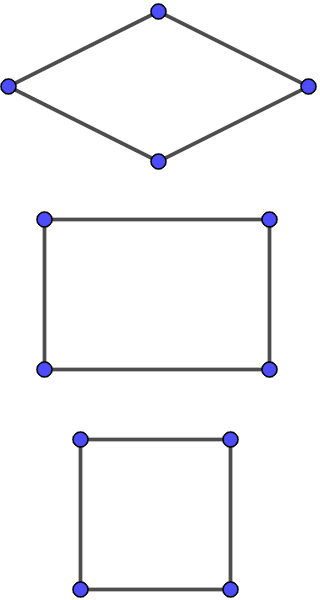
\includegraphics[width=0.24\textwidth]{tu/特殊平行四边形.png}
\end{wrapfigure}

把菱形沿对角线“裁开”，得到的一对三角形都是等腰三角形。
由于对角线平分，菱形的中心是等腰三角心底边中点，对角线也是中线。
而等腰三角形三线合一，中线就是高线。所以菱形的对角线不仅相互平分，而且相互垂直。

反过来，如果四边形的对角线相互平分，而且相互垂直，那么它是菱形。
菱形的两条对角线把它分为四个全等的直角三角形。

如果四边形四角相等，就说它是\textbf{矩形}或\textbf{长方形}。由于四边形内角和是周角，平行四边形对角相等，
所以也可以这样判定矩形：
\begin{tm}\label{tm:0-1-10}
    有一个角是直角的平行四边形是矩形。
\end{tm}

把矩形$ABCD$沿对角线$AC$“裁开”，得到$\triangle ABC$和$\triangle CDA$，
由于$\angle ABC$和$\angle CDA$都是直角，$\triangle ABC$和$\triangle CDA$是直角三角形。
根据勾股定理。$|AC|^2 = |AB|^2 + |BC|^2$。
另一方面，把矩形$ABCD$沿对角线$BD$“裁开”，通过类似推理可以得到：
$|BD|^2 = |AB|^2 + |AD|^2$。而$|BC| = |AD|$，所以$|AC| = |BD|$。即：
\begin{tm}\label{tm:0-1-15}
    矩形的对角线相互平分，而且等长。
\end{tm}

反过来，如果四边形的对角线相互平分而且等长，那么它是矩形。
矩形的两条把它分为两对全等的等腰三角形。

如果一个四边形既是菱形，又是矩形，就称它为\textbf{正方形}。
正方形是我们很熟悉的图形。正方形的四边等长，四个内角都是直角。
它的对角线长度是边长的$\sqrt{2}$倍。把正方形沿对角线“裁开”，得到一对等腰直角三角形。
正方形的两条对角线把它分为四个更小而全等的等腰直角三角形。

\section{梯形}
除了平行四边形，还有其他类型的四边形。

\begin{wrapfigure}[8]{r}{0.38\textwidth} %this figure will be at the right
    \vspace{-35pt}
    \centering
    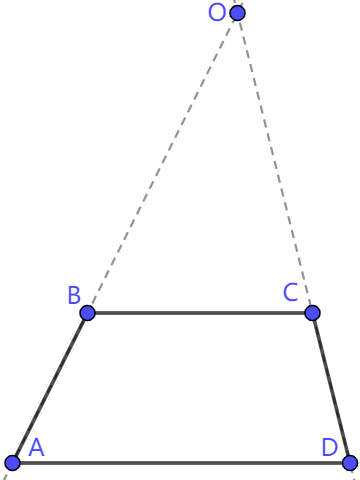
\includegraphics[width=0.36\textwidth]{tu/梯形1.png}
\end{wrapfigure}

如果四边形有一对边平行，就说它是\textbf{梯形}。如果梯形另一对边也平行，
就是平行四边形。我们已经研究过平行四边形了，所以，一般说梯形时，都指非平行四边形的梯形。

研究相似三角形的时候，我们已经接触过梯形。
如右图，大的三角形里去掉小的三角形，就是梯形。
把梯形补全为一对相似三角形，是常见的思考方式。

按照这个说法，梯形平行的一对边长度不等。我们称它们为\textbf{上底}和\textbf{下底}。
一般会把较短的一边称为上底，较长的称为下底。另外两条边一般称为梯形的\textbf{腰}。
两腰等长的梯形，称为\textbf{等腰梯形}。等腰梯形对应一对相似的等腰三角形。

设梯形$ABCD$中$BC \parallel AD$，那么同旁内角$\angle ABC + \angle DAB = 180^\circ$，
$\angle BCD + \angle CDA = 180^\circ$。如果其中一个角是直角，这样的梯形叫作\textbf{直角梯形}。
直角梯形对应一对相似的直角三角形。

梯形两腰的中点连线，称为梯形的\textbf{中位线}。
\begin{tm}\label{tm:0-2-20}
    梯形中位线长度是两底长度之和的一半。
\end{tm}
\begin{proof}
    设梯形$ABCD$中$BC \parallel AD$，$M$是边$AB$的中点，$N$是边$CD$的中点，
    直线$AB$、$CD$交于点$O$。由于$BC \parallel AD$，$\triangle OBC \sim \triangle OAD$。
    因此：
    $$ \frac{|OB|}{|OA|} = \frac{|OC|}{|OD|} = \frac{|BC|}{|AD|} = k.$$
    其中$k$是比例系数，即：
    $$ |OB| = k|OA|, \quad |OC| = k|OD|.$$
    于是
    $$ |OM| = |OB| + \frac{|AB|}{2} = \frac{|OA| + |OB|}{2} = \frac{k+1}{2} \cdot|OA|.$$
    同理，
    $$ |ON| = |OC| + \frac{|CD|}{2} = \frac{k+1}{2}\cdot|OD|. $$
    这说明
    $$ \frac{|OM|}{|OA|} = \frac{|ON|}{|OD|} = \frac{k+1}{2}. $$
    而$\angle MON = \angle AOD$，所以$\triangle OAD \sim \triangle OMN$。于是中位线$MN$的长度为
    $$ |MN| = |AD| \cdot \frac{|OM|}{|OA|} = \frac{k+1}{2}\cdot|AD|. $$
    将$k = \frac{|BC|}{|AD|}$代入，就得到
    $$ |MN| = \frac{|BC| + |AD|}{2}. $$
\end{proof}

\section{筝形}

\begin{wrapfigure}[6]{r}{0.32\textwidth} %this figure will be at the right
    \vspace{-5pt}
    \centering
    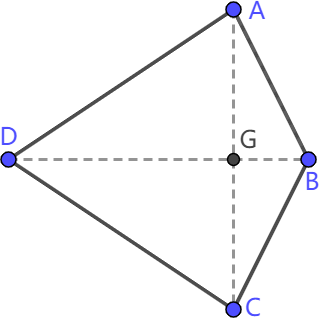
\includegraphics[width=0.32\textwidth]{tu/筝形1.png}
\end{wrapfigure}

平行四边形可以“裁成”两个同角全等的三角形。或者说，一对同角全等的三角形可以拼出一个平行四边形。
那么，一对反角全等的三角形拼出的图形是什么呢？

这个图形叫作\textbf{筝形}。我们对筝形并不陌生，在证明“角边角”的时候已经见过。
四边形的两对邻边分别等长，就叫作筝形。

如果筝形的对边也等长，就成了菱形。所以，一般说筝形时，都指非菱形的筝形。

筝形的最大特点，就是一条对角线是另一条的垂直平分线。我们把它叫作\textbf{脊线}，
把另一条（被它平分的）对角线叫作\textbf{肩线}。我们已经证明过，脊线和肩线相互垂直。
它们把筝形分为两对全等直角三角形。

直角坐标系中，把$(0,0)$、$(0,a)$、$(a,a)$、$(a,0)$四点依次连起来，就围成一个边长为$a$的正方形。
如果把$(0,0)$、$(0,b)$、$(a,b)$、$(a,0)$四点依次连起来，就围成一个长宽为$a$和$b$的矩形。
如果把$(-a,0)$、$(0,b)$、$(a,0)$、$(0,-b)$四点依次连起来，就围成一个菱形。
如果把$(0,0)$、$(a,b)$、$(a+u,b+v)$、$(u,v)$四点依次连起来，就围成一个平行四边形。
这些形状可以看作是实心的点集。比如以上正方形对应点集：
$$\{(x,y) \,|\, 0\leqslant x, y \leqslant a\}.$$

从$(0,0)$、$(0,a)$、$(a,a)$、$(a,0)$连成的正方形出发，关于点$(0, a)$平移，
就得到一个新的正方形，它是$(0,a)$、$(0,2a)$、$(a,2a)$、$(a,a)$连成的正方形。

\begin{sk}\label{sk:5-3-0}
    \mbox{}\\
    \indent 1. 从一个（实心）正方形出发，通过平移，能否填满整个平面，不留空隙也不互相重叠？\\
    \indent 2. 从一个（实心的）矩形、菱形、平行四边形出发，通过平移，能否填满整个平面，不留空隙也不互相重叠？\\    
    \indent 3. 如果从一个（实心）图形出发，用和它全等的图形可以填满整个平面，不留空隙也不互相重叠，就说它是\textbf{密铺图形}，可以密铺平面。
    正方形、矩形、菱形、平行四边形、等腰梯形、直角梯形、筝形，哪些是密铺图形？\\    
    \indent 4. 如果一个图形关于某条直线的轴对称图形是它自己，就说它是\textbf{轴对称图形}，该直线是它的对称轴。
    同样，如果一个图形关于某点的中心对称图形是它自己，就说它是\textbf{中心对称图形}，该点是它的对称中心。
    正方形、矩形、菱形、平行四边形、等腰梯形、直角梯形、筝形，哪些是轴对称图形，哪些是中心对称图形？
    它们分别有哪些对称轴和对称中心？
\end{sk}

\sectionext{剪形和蝶形}
比较以下的四边形，它们相应的角度有什么不同？

% 平行四边形、剪形和蝶形
\begin{figure}[H] 
    \vspace{4pt}
    \centering
    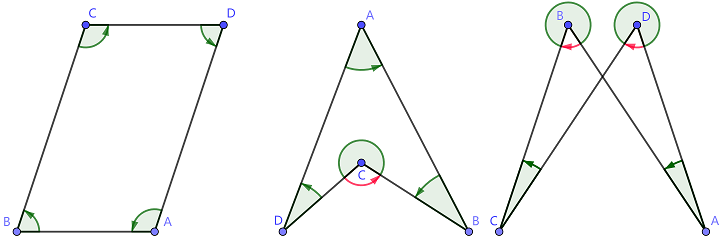
\includegraphics[width=0.8\textwidth]{tu/凹四边形1.png}
\end{figure}

给定四个点$A$、$B$、$C$、$D$，我们把线段$AB$、$BC$、$CD$、$DA$连起来的图形叫做四边形$ABCD$。
这四个顶点和四条边也组成了四个角：$\angle ABC$、$\angle BCD$、$\angle CDA$、$\angle DAB$。
我们称其为四边形$ABCD$的四个内角。

我们已经学习了平行四边形、梯形、筝形等四边形。如果把角的范围限定在\textbf{负平角}和\textbf{正平角}之间，
平行四边形的内角要么总是正的，要么总是负的。但也有一些四边形，它们的内角总是有正有负。
比如上图中间的四边形，内角$\angle BCD$是负的；上图右边的四边形，内角$\angle ABC$和$\angle CDA$是负的。

如果把这些四边形作轴对称，得到的四边形内角恰好与原本相反。上图中间的四边形会变成有三个内角为负的四边形；
右边的四边形仍旧是两个内角为负的四边形。

我们把类似上图中间的四边形，内角中有一个或三个为负的，称为\textbf{剪形}；
把类似上图右边的四边形，内角中有两个为负的，称为\textbf{蝶形}。

蝶形和剪形合称为\textbf{凹四边形}，其余内角总为正或总为负的四边形，称为\textbf{凸四边形}。
平行四边形总是凸四边形。梯形也可以是蝶形，筝形也可以是剪形。

\begin{sk}\label{sk:5-4-0}
    \mbox{}\\
    \indent 1. 梯形在什么情况下是蝶形？画一个例子。\\
    \indent 2. 筝形在什么情况下是剪形？画一个例子。\\
    \indent 3. 考虑四边形内角的正负。凸四边形的内角是“正-正-正-正”或“负-负-负-负”；
    剪形的内角是“正-正-正-负”或“正-负-负-负”；蝶形的内角是“正-正-负-负”。是否有其他的可能组合？
    哪些正负组合是不可能的？为什么？
\end{sk}

\section{四边形的面积}
学习了各种常见的基本图形后，最后来看它们的面积。我们已经学习过正方形、矩形、平行四边形和三角形的面积公式。
现在，我们把这些性质归纳成公理。

\begin{wrapfigure}[4]{r}{0.36\textwidth} 
    \vspace{-30pt}
    \flushright
    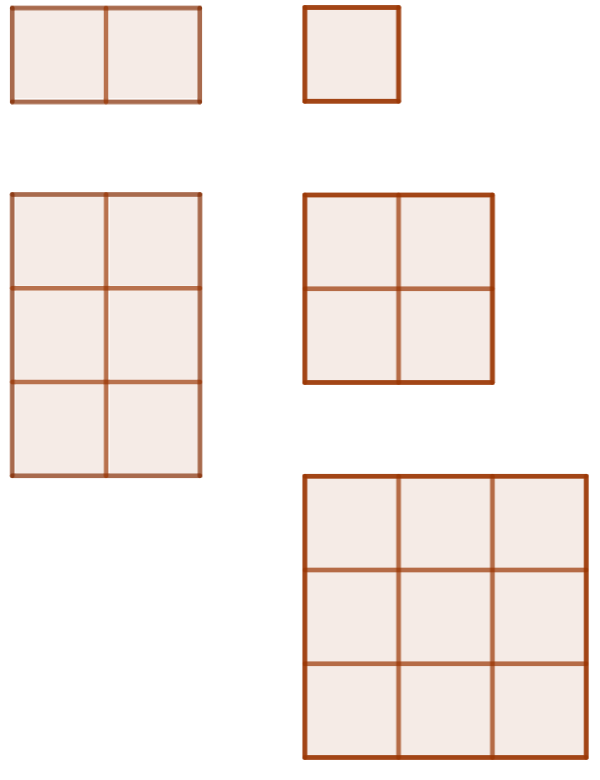
\includegraphics[width=0.32\textwidth]{tu/面积_矩形1.png}
\end{wrapfigure}

我们把正方形作为面积的单位。
\begin{po}
    边长为一的正方形，面积为一。
\end{po}

我们把边长为一的正方形称为\textbf{单位正方形}。怎样从单位正方形得到其他图形的面积呢？

回顾（右图）：我们是怎样数出正方形乃至矩形面积的。

\begin{po}
    图形的面积是其各部分面积之和。
\end{po}

\begin{po}
    图形平移、旋转后，面积不变。对称的图形，面积相等。
\end{po}
这两个公理给出了从单位正方形得到其他图形的面积的方法。
从单位正方形出发，我们可以得到矩形、平行四边形、三角形的面积公式。

\begin{figure}[H] %this figure will be at the right
    \vspace{4pt}
    \centering
    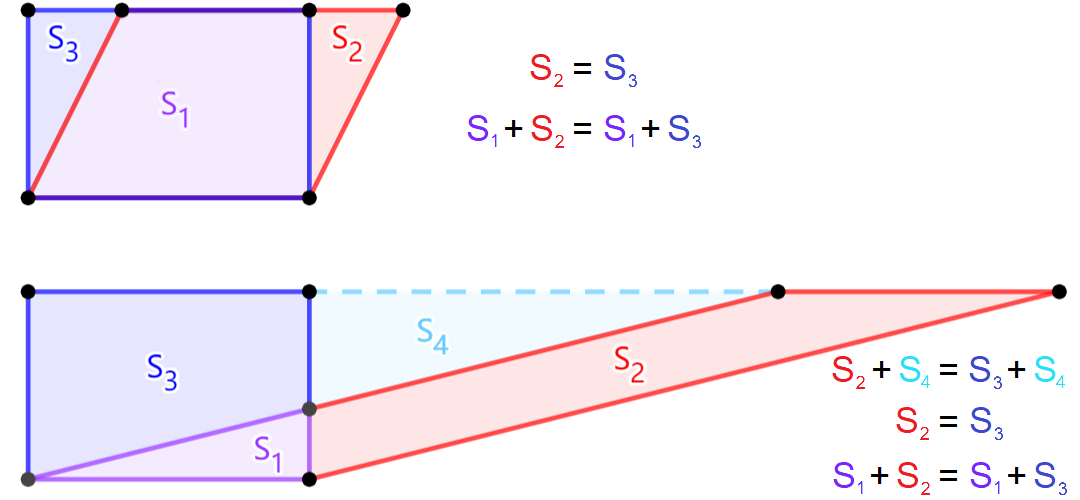
\includegraphics[width=0.6\textwidth]{tu/面积_平行四边形1.png}
\end{figure}

\begin{itemize}
    \item 正方形的面积等于边长的平方。
    \item 矩形的面积等于长乘宽。
    \item 平行四边形的面积等于同底等高的矩形的面积，即底乘高。
    \item 三角形的面积是同底等高平行四边形的一半，即底乘高的一半。
\end{itemize}

同底等高的平行四边形的面积，都等于和它们同底等高的矩形的面积。
同底等高的三角形的面积，分别为同底等高的平行四边形的面积的一半。因此我们得出熟知的结论：
\begin{tm}
    同底等高的平行四边形面积相等。同底等高的三角形面积相等。
\end{tm}

梯形的面积，可以通过将两个梯形拼成一个平行四边形而求得。
筝形的面积，可以通过将对角线分成的四个三角形旋转，拼成矩形而求得。

\begin{figure}[H] 
    \vspace{4pt}
    \centering
    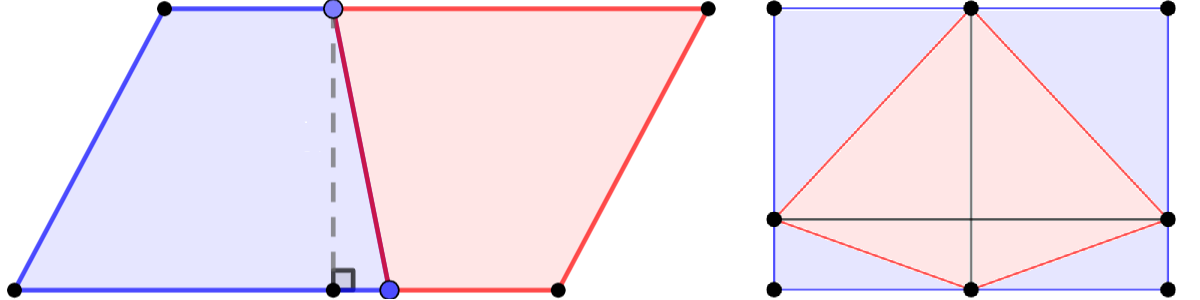
\includegraphics[width=0.8\textwidth]{tu/面积_梯形1.png}
\end{figure}

\begin{itemize}
    \item 梯形的面积等于上下底边长之和乘高除以2。
    \item 筝形的面积等于对角线乘积的一半。
\end{itemize}

怎样求一般的四边形，乃至多边形的面积呢？讨论四边形内角和的时候，我们已经发现，
可以沿着对角线把任何多边形划分成若干个三角形。因此，四边形乃至多边形的面积，就是这些三角形面积之和。
也就是说，只要能够求出任意形状三角形的面积，就能求出任意四边形乃至多边形的面积。
这个问题我们将会在后续章节中讨论。

多边形是由线段首尾相接连成的。
如果平面图形的边不是线段，如何讨论它们的面积呢？

观察下图，图形完整覆盖了多少个方格？有多少个方格覆盖了图形？你有什么想法？

\begin{figure}[H] 
    \vspace{4pt}
    \centering
    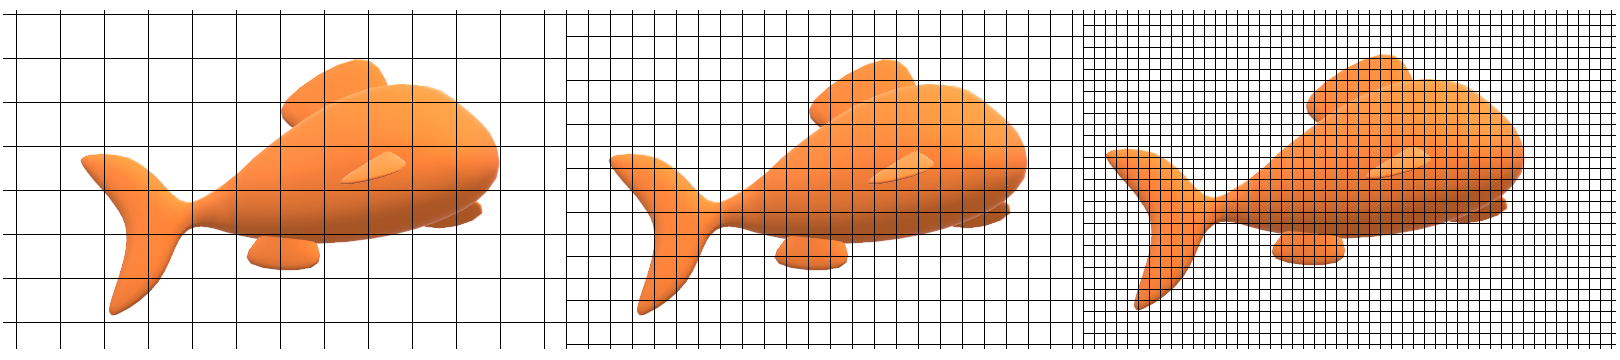
\includegraphics[width=0.8\textwidth]{tu/面积_鱼1.png}
\end{figure}

上图中，我们把一张透明方格网纸放在图形上。图形的面积$S$大于等于它完整覆盖的方格数$N_{\text{内}}$，
同时小于等于把它完整覆盖所用的方格数$N_{\text{外}}$。设每个方格面积为$S_1$，
那么$S$介于$N_{\text{内}}S_1$和$N_{\text{外}}S_1$之间。如果随着方格面积缩小，
$N_{\text{内}}S_1$和$N_{\text{外}}S_1$的差也逐渐缩小，那么我们就能越来越精确地估计图形的面积。

\begin{sk}
    \mbox{} \\
    \indent 1. 是否所有平面图形都有面积？怎样界定一个图形是否有面积？
\end{sk}

\begin{xt}
    \mbox{} \\

    \begin{figure}[H] 
        \vspace{4pt}
        \centering
        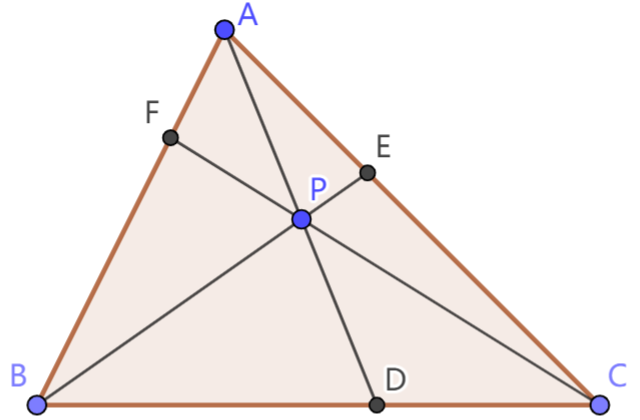
\includegraphics[width=0.45\textwidth]{tu/塞瓦定理1.png}
    \end{figure}

    \indent 1. 给定三角形$ABC$及其内一点$P$，从三角形各个顶点出发的射线$AP$、$BP$、$CP$
    分别交对边$BC$、$AC$、$AB$于$D$、$E$、$F$。\\
    \indent 1.1 证明：
    $$ \frac{|AF|}{|FB|} = \frac{S_{\triangle ACF}}{S_{\triangle FCB}}\,\,.$$
    \indent 其中$S_{\triangle ACF}$表示三角形$ACF$的面积。下同。\\
    \indent 1.2 证明：
    $$ \frac{|AF|}{|FB|} = \frac{S_{\triangle ACP}}{S_{\triangle PCB}}\,\,.$$
    \indent 1.3 证明：
    $$ \frac{|AF|}{|FB|} \cdot \frac{|BD|}{|DC|} \cdot \frac{|CE|}{|EA|} = 1\,\,.$$
    \indent 1.4 证明：
    $$ \frac{|AP|}{|PD|} = \frac{S_{\triangle ACP}}{S_{\triangle PCD}}\,\,.$$
    \indent 1.5 证明：
    $$ \frac{|AP|}{|PD|} \cdot \frac{|DC|}{|CB|} \cdot \frac{|BF|}{|FA|} = 1\,\,.$$
    \indent 1.6 你还能发现哪些类似的等式？
\end{xt}


\chapter{数的分解}
自然数是我们最早认识的数。我们已经熟悉了自然数的四则运算，并且学习了因数和倍数。
了解一个数的因数，无论对于理论研究，还是在实际生活中，都很有用处。
\section{初识素数}
我们已经学习过因数的概念。我们把因数只有自己和$1$的正整数叫做\textbf{素数}，
除了$1$和自己还有别的因数的正整数叫做\textbf{合数}。约定$1$既不是素数也不是合数。

举例来说，$2$、$3$、$5$、$7$是素数，而$4$、$6$、$8$是合数。偶素数只有一个：$2$，其余素数都是奇数。

\begin{tm}\label{tm:1-0-0}
    设$p$是素数。任何正整数要么是$p$的倍数，要么与$p$互素。
\end{tm}
\begin{proof}
    设$n$是正整数。记$n$和$p$的最大公因数为$d$。$d$是$p$的因数。
    因此按$p$的定义，要么$d = p$，要么$d = 1$。
    如果$d = p$，那么$n$是$p$的倍数。如果$d = 1$，那么$n$与$p$互素。
\end{proof}

素数与合数有什么关系呢？

\begin{tm}\label{tm:1-0-4}
    合数总有素因数。
\end{tm}
\begin{proof}
    按照定义，合数总有真因数。给定合数$n$，它的真因数大于$1$、小于$n$，至少有一个，至多有$n-2$个。
    其中总有一个最小的真因数，我们把它记为$p$。\\
    $p$的因数也是$n$的因数，所以要么是$1$，要么大于等于$p$。也就是说，$p$没有真因数。所以$p$是素数。
\end{proof}

\begin{tm}\label{tm:1-0-6}
    每个大于$1$的整数都可以表示成素数或其乘积。
\end{tm}
\begin{proof}
    使用归纳法。命题$P(n)$：整数$n$可以表示成素数或其乘积。下面证明$P$对每个大于$1$的整数成立。\\
    $n=2$时，由于$2 = 2$，$P(2)$成立。\\
    假设对某个大于$1$的整数$n$，$P(2), \cdots, P(n)$都成立，下面证明$P(n+1)$也成立。\\
    如果$n+1$是素数，那么$n+1 = n+1$就是素数，于是$P(n+1)$成立。\\
    如果$n+1$是合数，那么它至少有一个素因数$p$。设$n+1 = mp, m\in\mathbb{Z}^+$，
    由于$1<p<n+1$，所以$1< m < n+1$。根据假设，$P(m)$成立，也就是说，
    $m$可以表示成素数或其乘积：
    $$ m = p_1 p_2\cdots p_k, \,\,\, l\in\mathbb{Z}^+$$
    于是，$n+1 = mp = pp_1 p_2\cdots p_k$也是素数的乘积。于是$P(n+1)$成立。\\
    综上所述，$P(n)$对每个大于$1$的整数成立。
\end{proof}

我们把这种表示正整数的方式称为\textbf{素因数分解}。
如果把自然数比作一座座房屋，那么素数就是砖瓦，构建起一个个合数。

素数与合数，谁比较多呢？一位数中，有$4$个素数，$4$个合数；二位数中，有$21$个素数，$69$个合数；
三位数中，有$143$个素数，$757$个合数；四位数中有$1061$个素数，$7939$个合数。

越大的素数，越是罕见。

会不会从某个数开始，所有比它大的都是合数？也许，素数只有有限个？我们有这样一个定理：

\begin{tm}\label{tm:1-0-10}
    素数的个数是无穷的。
\end{tm}
\begin{proof}
    使用反证法证明。反设素数的个数不是无穷的，即只有有限多个素数。把素数的个数记为$N$，把它们从小到大分别记为
    $p_1, p_2,\cdots , p_N$。\\
    考察这样的正整数：
    $$ m = p_1p_2\cdots p_N + 1.$$
    $m$与所有素数互素。所以，$m$的因数要么是$1$，要么是它自己，要么是某个与$p_1$、$p_2$、……、$p_N$都不一样的数。
    这就说明，要么$m$自己是素数，要么它的因数中有和$p_1, p_2,\cdots , p_N$都不一样的素数。
    这就和“素数一共有$N$个”矛盾了。\\
    因此，原命题的否定“素数的个数不是无穷的”是假的，原命题成立。
\end{proof}

素数作为“砖瓦”的性质，还体现在以下定理中：
\begin{tm}{\textbf{存因定理 }}\label{tm:1-0-20}
    如果素数$p$整除两个自然数$a$和$b$的乘积：$p | ab$，那么$p$整除$a$或$p$整除$b$。
\end{tm}
\begin{proof}
    给定符合条件的素数$p$和自然数$a,b$。如果$p$整除$a$，那么命题得证。\\
    如果$p$不整除$a$，那么由于两者的最大公因数是$p$的因数，因此只能是$1$。两者互素。
    根据倍和析因定理，存在整数$m,n$使得
    $$ mp + na = 1.$$
    两边乘以$b$，就得到：
    $$ mp + nab = b. $$
    根据已知条件，存在整数$k$使得$ab = kp$，于是 
    $$ b = mp + nkp = (m + nk)p,$$
    即$p$整除$b$。
\end{proof}

存因定理告诉我们，如果某个正整数$n$有素因数$p$，把$n$“拆成”两个数的乘积，那么总有一个有素因数$p$。
反复运用存因定理，我们可以把这个结论加强：无论把$n$“拆成”几个数的乘积，总有一个有素因数$p$。
这反映了素数作为自然数中的“砖瓦”的性质。

\begin{xt}\label{xt:1-0-0}
    证明：\\
    \indent 1. 两个素数要么相等，要么互素。\\
    \indent 2. 如果素数$p$整除完全平方数$n$，那么$p^2$也整除$n$。\\
    \indent 3. 设$p,q$是素数，$i,j$是正整数，那么要么$p^i$和$q^j$互素，要么$p^i$整除$q^j$，要么$q^j$整除$p^i$。\\
    \indent 4. 对任何正整数$n$，都存在$n$个连续合数$a, a+1, \cdots , a+n-1$。
\end{xt}

\section{算数基本定理}
从存因定理出发，可以得到一个很重要的结论：
\begin{tm}{\textbf{算术基本定理}}\label{tm:1-1-0}
    如果不考虑素因数的排列顺序，素因数分解的方式是唯一的。
\end{tm}
\begin{proof}
    如果某个大于$1$的整数$n$有两种素因数分解。把每种分解的素因数从小到大排列：
    $$ n = p_1p_2\cdots p_k = q_1q_2\cdots q_l, \,\,\, k, l \in \mathbb{Z}^+.$$
    我们要证明这两种分解是一样的。\\
    考虑$p_1$，$p_1$整除$n = q_1q_2\cdots q_l$。根据存因定理，存在某个$j$使得$p_1$整除$q_j$。
    $q_j$也是素数，所以$p_1$不可能是它的真因数。于是$p_1 = q_j \geqslant q_1$。\\
    考虑$q_1$，按照相同的推理，存在某个$i$使得$q_1$整除$p_i$。于是$q_1 = p_i \geqslant p_1$。\\
    因此，$p_1 = q_1$。\\
    我们把$n$除以$p_1$，得到正整数$n_1$。如果$n_1 = 1$，那么我们有$n_1 = p_1$，分解方式是唯一的。
    如果$n_1 = p_2\cdots p_k = q_2\cdots q_l > 1$，我们可以再次运用以上的推理，得到：$p_2 = q_2$。\\
    以此类推，经过有限步后，我们可以得到：$k=l$，且
    $$p_1 = q_1, \,\,\, p_2 = q_2, \, \cdots \, , p_k = q_k.$$
    也就是说，$n$的素因数分解只有一种方式。
\end{proof}

这个结论非常重要，我们把它称为算术基本定理。算术基本定理告诉我们，不考虑排列顺序的话，
每个大于$1$的正整数都可以用唯一的方式写成素数或其乘积。这种唯一的方式可以看作每个正整数的
“身份证”。为了方便讨论，素因数分解中，一般素因数从小到大排列，并用乘方的形式合并相同的素因数。
比如，$252$的素因数分解写成；
$$ 252 = 2^2 \cdot 3^2 \cdot 7^1.$$
这种写法称为数的\textbf{标准分解}。以上就是$252$的标准分解。
有时候，为了便于讨论，我们会把不是$n$的因数的素数也写进分解表达式里，用它的$0$次方“占位”.比如$210$
就可以写成：
$$ 252 = 2^2 \cdot 3^2 \cdot 5^0 \cdot 7^1.$$
这样的写法，在规定了涉及的素数集合后，仍然是唯一的。

\begin{xt}\label{xt:1-1-0}
    写出以下数的标准分解：\\
    \indent 1. $256, 243, 125$.\\
    \indent 2. $60, 780, 1296$.\\
    \indent 3. $1001, 5929, 8801$.
\end{xt}

把正整数$n$分解，得到：$n = p_1^{u_1} p_2^{u_2} \cdots p_k^{u_k}$。
我们把$u_1$称为$p_1$在$n$中的重数。它是让$p_1^i$整除$n$的最大自然数$i$。
\begin{tm}\label{tm:1-1-10}
    如果$n$整除$m$，那么任何素数在$n$中的重数小于等于它在$m$中的重数。
\end{tm}
\begin{proof}
    设素数$p$在$n$和$m$中的重数分别是$u$和$v$。于是$p^u$整除$n$，因而整除$m$。
    另一方面，$v$是让$p^i$整除$m$的最大自然数$i$。所以，$u \leqslant v$。
\end{proof}

上面的结论也可以换个方式说成：如果$n$是$m$的因数，那么任何素数在$n$中的重数小于等于它在$m$中的重数；
如果$n$是$m$的倍数，那么任何素数在$n$中的重数大于等于它在$m$中的重数。

\begin{tm}\label{tm:1-1-20}
    正整数$n,m$的乘积，等于它们的最大公因数和最小公倍数的乘积。
\end{tm}
\begin{proof}
    设$n,m$的最大公因数是$d$，最小公倍数是$q$，下面证明$nm = dq$。\\
    把$n,m,d,q$分解，设涉及的素数为$p_1, p_2, \cdots , p_k$。把四个数分别记为：
    \begin{align*}
        n &= p_1^{u_1}p_2^{u_2}\cdots p_k^{u_k}, \quad m = p_1^{v_1}p_2^{v_2}\cdots p_k^{v_k},  \\
        d &= p_1^{s_1}p_2^{s_2}\cdots p_k^{s_k}, \quad q = p_1^{t_1}p_2^{t_2}\cdots p_k^{t_k}.  
    \end{align*}
    $d$既是$n$的因数也是$m$的因数，所以对每个素因数$p_i$，它在$d$中的重数$s_i$都小于等于$u_i$和$v_i$。
    同时，由于$d$是最大公因数，所以$s_i$是$u_i$和$v_i$中较小的数。\\
    $q$既是$n$的倍数也是$m$的倍数，所以对每个素因数$p_i$，它在$q$中的重数$t_i$都大于等于$u_i$和$v_i$。
    同时，由于$q$是最小公倍数，所以$t_i$是$u_i$和$v_i$中较大的数。\\
    因此，对每个素因数$p_i$，$s_i + t_i = u_i + v_i$。于是，
    \begin{align*}
        nm &= \left(p_1^{u_1}p_2^{u_2}\cdots p_k^{u_k}\right) \cdot \left(p_1^{v_1}p_2^{v_2}\cdots p_k^{v_k}\right)  \\
        &= p_1^{u_1 + v_1}p_2^{u_2 + v_2}\cdots p_k^{u_k + v_k}  \\
        &= p_1^{s_1 + t_1}p_2^{s_2 + t_2}\cdots p_k^{s_k + t_k}  \\
        &= \left(p_1^{s_1}p_2^{s_2}\cdots p_k^{s_k}\right) \cdot \left(p_1^{t_1}p_2^{t_2}\cdots p_k^{t_k}\right)  \\
        &= dq 
    \end{align*}    

\end{proof}

\begin{xt}\label{xt:1-1-1}
    \mbox{}\\
    \indent 1. 设$i$是素数$p$在正整数$n$中的重数。\\
    \indent 1. 1. 如果$p$不整除$n$，证明$i = 0$。\\
    \indent 1. 2. 如果自然数$j < i$，证明：$p^j$整除$n$。\\
    \indent 1. 3. 如果自然数$j > i$，证明：$p^j$不整除$n$。\\
    \indent 2. 设正整数$n,m$的最大公因数是$d$，素数$p$在$d,n,m$中的重数分别是$s,u,v$。\\
    \indent 2. 1. 设$v$是$u,v$中较小的数，证明：$s \leqslant v$。\\
    \indent 2. 2. 假设$s < v$，考虑$pd$，证明$pd$是$n,m$的公因数。\\
    \indent 2. 3. 证明$s$等于$u,v$中较小的数。 \\
    \indent 2. 4. 设正整数$n,m$的最小公倍数是$q$，素数$p$在$q,n,m$中的重数分别是$t,u,v$，证明：$t$等于$u,v$中较大的数。\\
\end{xt}

给定一个正整数，如何将它分解呢？这个问题一直困扰着人类。将非常大的整数分解，是一项非常困难的任务。
即便在现代，电子计算机计算能力有极大发展，可以轻易做到每秒百亿乃至万亿次运算，分解大整数仍然需要非常多的时间。
一些常用的密码技术，就依赖于分解大整数非常困难这个事实。

如今，量子计算理论不断发展。人们将希望寄于量子计算机，认为将来使用量子计算机及相应的算法，
可以在合理时间内分解大整数。

\chapter{因式分解}
整式是变量和数量作加减法和乘法得到的代数式。它的性质和整数很相似。
整数可以分解成因数的乘积，整式也可以分解为整式的乘积。
把整式的乘积写成若干项的和，叫做整式的展开；
反过来，把一个整式写成多个整式的乘积，称为整式的\textbf{因式分解}。乘积中每个整式称为原整式的\textbf{因式}。

整式的因式分解是一个非常庞大的问题。我们只从最简单的情况出发，归纳一些特殊情况下的简单方法。

\section{一元整式}
一种简单的情况是一元整式的因式分解。给定变量为$x$的一元整式$p$，合并同类项后按照次数从高到低排列，可以写成：
$$ p = a_nx^n + a_{n-1}x^{n-1} + \cdots + a_1 x + a_0.$$
其中$a_0, a_1, \cdot , a_n$都是有理数，称为$p$的系数。其中$a_n$不等于$0$，而其它数可能等于$0$。
$a_nx^n$称为$p$的\textbf{最高次项}，$a_n$就是最高次项的系数，$n$称为$p$的次数。比如$n=1$时，$p$
就是我们见过的一元一次式。$n=0$时，$p$只有常数项，称为常式。为了强调$p$是关于$x$的一元式，我们也将$p$记为$p(x)$。

给定一元整式$n(x)$和$m(x)$，如果$n(x)$可以写成$m(x)$和另一个一元整式$q(x)$的乘积，
就说$n(x)$是$m(x)$的\textbf{倍式}，$m(x)$是$n(x)$的\textbf{因式}。

和整数一样，一元整式也有带余除法。整式的带余除法可以和整数除法一样，用竖式计算。
比如$8x^5 +2x^4 -9x^3+ 4x-5$除以$2x^2+x-1$：
$$\polylongdiv{8x^5 +2x^4 -9x^3+ 4x-5}{2x^2+x-1}$$
可以看到，\textbf{被除式}$8x^5 +2x^4 -9x^3+ 4x-5$除以\textbf{除式}$2x^2+x-1$，得到\textbf{商式}$4x^3-x^2-2x+\frac12$和\textbf{余式}$\frac32 x- \frac92$。
竖式除法中，不同次数的项就好像整数的个十百千等数位。不同的是相减的时候没有借位，而且由于系数可以是分数，
所以只要剩下的式子的次数不少于除式，就可以继续相减。最后得到的余式，次数一定严格小于除式。
\begin{sk}\label{sk:2-0-0}
    整式$p(x)$除以一次式，余式是怎样的？除以常式呢？
\end{sk}
\begin{xt}\label{xt:2-0-0}
    计算带余除法：\\
    1. $x^3 - 3x^2 + 2x - 5$除以$x^2 + x + 2$。\\
    2. $x^6 - x^5 - 4x^3 + 11x^2 - 9x + 19$除以$x^3 - 2x^2 + x + 4$。
\end{xt}

\section{试根法}
怎么样找到一元整式的因式呢？我们来看上面的整式除法。

当$x=1$的时候，$2x^2+x-1 = 2$，$8x^5 +2x^4 -9x^3+ 4x-5 = 0$，
$4x^3-x^2-2x+\frac12 = \frac32$，$\frac32 x- \frac92 = -3$。
带余除法变成：$0 = 2 \cdot \frac32 - 3$。

用特定的数值代替$x$，整式的带余除法就变成整数的带余除法。如果$x$取某个值使得除式$2x^2 + x - 1 = 0$，
比如$x = -1$，那么带余除法变成：$-6 = 0\cdot \left(\frac52\right) - 6$。

如果$2x^2 + x - 1$是某个一元整式$p(x)$的因式，
$$ p(x) = (2x^2 + x - 1)q(x)$$
那么，某个$x$的取值（比如$-1$）使得$2x^2 + x - 1 = 0$的时候，上式变成：
$$ p(-1) = 0 \cdot q(-1) = 0$$
如果某个数$a$使整式的因式等于$0$，那么它也使得整式为$0$。

使整式为$0$的数叫做整式的\textbf{根}。

如果某个数$a$使除式为$0$，被除式也为$0$，除式是否就是被除式的因式呢？
考虑带余除法：
$$\polylongdiv{8x^5 +2x^4 -9x^3+ 4x+1}{2x^2+x-1}$$
$x = -1$的时候，除式和被除式都是$0$，但这是由于$x = -1$时余式也是$0$。
除式并不是被除式的因式。

不过，如果余式是常式，那么它是不是$0$，就和$x$的取值无关了。
一种特殊情况是：除式是一次式：$x - a$。它只在$x$取值为$a$的时候为$0$。
这时，如果被除式也是$0$，那么余式肯定是$0$。于是除式是被除式的因式。
\begin{tm}\textbf{余式定理}\label{tm:2-1-0}
    \mbox{} \\
    如果$a$是一元整式$p(x)$的根，那么$x-a$是它的因式。
\end{tm}

\begin{xt}\label{xt:2-1-0}
    \mbox{}\\
    设有整式$p = 6x^3 - 3x^2 + 2x - 1$：\\
    \indent 1. 试着分解$p$。\\
    \indent 2. 如果既约分数$\frac{a}{b}$是$p$的根，证明：$|b|$整除$6$。\\
    设有整式$p = x^3 - 4x^2 - x - 20 $：\\
    \indent 1. 试着分解$p$。\\
    \indent 2. 如果既约分数$\frac{a}{b}$是$p$的根，证明：$|a|$整除$20$。\\
    如果既约分数$\frac{a}{b}$是整式$p = a_nx^n + a_{n-1}x^{n-1} + \cdots + a_1 x + a_0$的根，
    $a$和$b$应该满足什么条件？
\end{xt}

\section{一般整式的分解}
对一般的整式来说，也有一些普遍适用的方法。

\noindent \textbf{提公因式法}

\indent 如果要分解的整式中有显然的公因式，那么可以将它提取出来。比如：
$$ x^6 - 2x^4 + 19 x^3 -3x$$
\indent 以上这个式子中，每一项显然都有$x$作为因式。因此，可以分解为：
$$ x(x^5 - 2x^3 + 19x^2 - 3).$$
\indent 提公因式法是分配律的逆应用。

\noindent \textbf{公式法}

\indent 如果可以注意到要分解的整式是某个公式的展开形式，那么应用公式，
\indent 就可以把展开的形式还原成因式的成绩形式。比如： 
$$x^4 + 4$$
\indent 这个式子可以看成两个平方的差：
$$ x^4 + 4 = x^4 - 4x^2 + 4 - 4x^2 = (x^2 - 2)^2- (2x)^2.$$
\indent 于是，使用$a^2 - b^2 = (a + b)(a - b)$这个公式，就可以得到：
$$x^4 + 4 = (x^2 - 2 + 2x)(x^2 -2 -2x).$$
\indent 应用公式法，取决于要分解的整式是否符合某个特定公式的展开形式。

\noindent \textbf{分组分解法}

\indent 分组分解的思想是从提公因式法出发。如果不能发现显然的公因式，
\indent 就分组考察整式的项，看看是不是有哪些项可以先提取公因式。比如：
$$ ab + abc - a^2 - b^2c$$
\indent 可以先把上式的项分为两组：
$$ ab + abc - a^2 - b^2c = (ab - a^2) + (abc - b^2c)$$
\indent 然后分别对每一组做因式分解：
$$ ab + abc - a^2 - b^2c = (ab - a^2) + (abc - b^2c) = a(b - a) + bc(a - b)$$
\indent 然后再提取公因式$a - b$：
$$ ab + abc - a^2 - b^2c = a(b - a) + bc(a - b) = (a - b)(-a + bc).$$
\indent 可以看到，分组分解的关键在于：各组各自分解的结果，应该有共同的\\
\indent 因式。比如上式分成两组，每组都分解出了$a - b$这个因式。

\noindent \textbf{待定系数法}

\indent 如果对因式分解的结果有一定的猜测，可以先用变量代替暂时不知道\\
\indent 的系数，写出因式乘积。展开后，通过对比各项，得到系数。比如：
$$ 3ab + ac - a^2- bc -2b^2 $$
\indent 上式中，让$a = b$，则式子变为：
$$ 3ab + ac - a^2- bc -2b^2 = 3b^2 + bc - b^2- bc -2b^2 = 0$$
\indent 所以，猜测$a - b$是因式。由于式子最高次项次数是$2$，猜测因式分解\\
\indent 结果为：
$$ 3ab + ac - a^2- bc -2b^2 = (a - b)(ua + vb + wc).$$
\indent 展开后得到：
$$ 3ab + ac - a^2- bc -2b^2 = ua^2 + vb^2 + (v - u)ab + wac - wbc. $$
\indent 对比左右各项，得到$u = -1$、$v = 2$、$w = 1$。即：
$$ 3ab + ac - a^2- bc -2b^2 = (a - b)(-a + 2b + c).$$
\indent 待定系数法建立在对因式分解结果的合理猜测上。如果猜测出现错误，
\indent 后面对比各项时就会发现矛盾。

\chapter{估算和科学计算}

我们已经学习过整数和有理数的加减乘除运算。给定了确切的数值，我们能对它进行计算，得到准确的结果。不过，在生产和生活中，尤其是科学研究中，很多时候我们并不知道确切的数值，同时，我们只想快速地知道大致的计算结果，而不需要获得准确的计算结果。这时，我们需要掌握一些节省时间和精力的估算方法。

\begin{ex}
    小李在野外探险时遇到一棵树，他想知道树大概有多高。由于手边没有测量工具，小李无法直接测量树有多高。他使用“拇指法”来估计树的高度。他从树下直走$100$步后，转身伸出大拇指瞄准树，并朝着树前后走动，记录步数。当走到离树$120$步时，大拇指正好覆盖小李眼中的树。于是小李这样来估计树高：他大步走时的步长和自己的臂长大致相等。树离自己$120$步时，大拇指正好覆盖自己眼中的树，因此，树高是大拇指长度的$120$倍。小李估计自己的大拇指长度约为$4$厘米，所以树高约$4.8$米。
\end{ex}

\begin{figure}[h]
    \vspace{4pt}
    \centering
    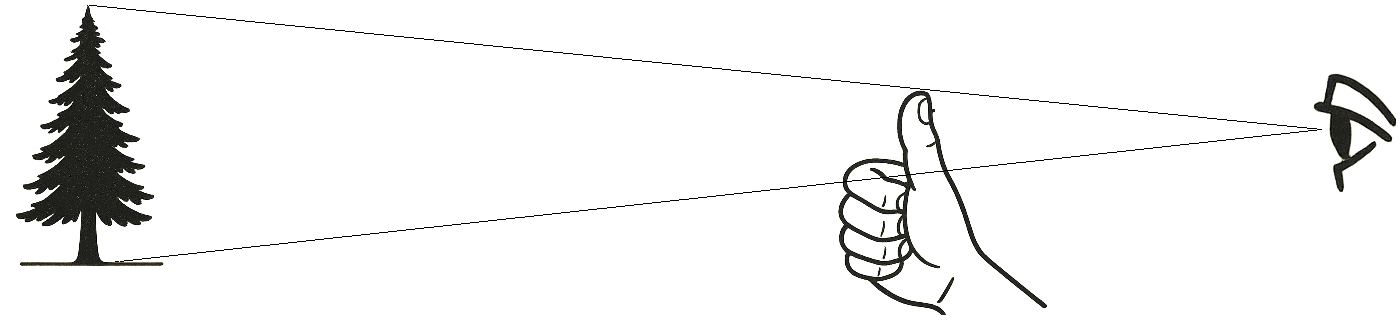
\includegraphics[width=0.9\textwidth]{tu/tree_measure1.png}
    \caption*{\texttt{用“拇指法”估计树的高度}}
\end{figure}

以上的例子里，小李对一棵树的高度做估计。他构思了一种估算方法，从自身出发，估计自己的步长、臂长和大拇指长度，再用这些数来算出树高。这种方法不会得到树的准确高度，但能够让小李对树的高度有大致的认识，在生活和生产、研究中都能带来很大的方便。

\begin{ex}
    小王到市场采购企业生产所需的零件。他的预算是$40$万元人民币。他分别向甲、乙、丙三家供应商询价，得知$A,B,C$三种零件的价格分别是：
    \begin{table}[htbp]
        \centering
        \label{tab:报价表}
        \begin{tabular}{|c|c|c|c|}
            \hline
            \textbf{供应商} & \textbf{A 零件} & \textbf{B 零件} & \textbf{C 零件} \\
            \hline
            \textbf{甲} & $2.95$ 元 & $16.5$ 元 & $43.5$ 元 \\
            \hline
            \textbf{乙} & $2.8$ 元 & $19.5$ 元 & $40.5$ 元 \\
            \hline
            \textbf{丙} & $2.9$ 元 & $17.5$ 元 & $42.5$ 元 \\
            \hline
        \end{tabular}
    \end{table}

    按照对业务的理解，小王估计三种零件的采购比例大致是$6$比$2$比$1$，也就是每个$C$零件大约要配$2$个$B$零件和$6$个$A$零件。以这样的比例，小王估算甲、乙、丙三家供应商对每套零件报价大约是：
    $$ 3\times 6 + 20 \times 2 + 40\times 1 = 98 \;\mbox{（元），} $$
    按每套$100$元估计，小王判断：以当前报价和自己的预算，至少可以买$4000$套零件。
\end{ex}

以上的例子里，小王并没有准确计算三家供应商关于一套零件的准确报价，而是大致取整后计算。然后用总预算除以一套零件的单价，得到了大约能买到的零件数量。这种做法能让小王在多变的市场里更好地抓住机会，达成交易。

\section{概数和误差}

前面的例子里，我们可以看到，为了方便快速计算，我们常常会放弃使用确切的数值，而使用大小差不多但容易算的数。这样的做法叫\textbf{取概数}。确切的数则称为\textbf{确数}。

概数一般取整数乃至十的倍数、一百的倍数等等。特别是做乘除法时，我们希望概数里非零的数字越少越好。比如，和$52 \times 68$相比，$50\times 70$更容易算。和$312.6 \times 7810$相比，$300 \times 8000$更容易算。概数通常用四舍五入法取得。如果时间紧急，直接用进一法或去尾法也可以。

使用概数来估算，结果往往就和准确计算的结果不一样了，会产生误差。快速估计误差，也是必要的。这让我们能够权衡为了快速计算，付出了什么代价。

估计误差，有两个关键：方向和大小。如果能确认和正确的结果相比，估算的结果是大了还是小了，那么对正确的结果就有更清晰的把握。前面买零件的例子里，小王要向供应商下单购买零件，所以他希望估计的结果比正确结果更小。比如说，如果小王通过估计误差知道一套零件报价不超过$100$元，那么他就能估计出$4000$套零件比正确的结果小，实际用$40$万元预算能买的零件套数应该比$4000$更大。这样他可以放心地向供应商下单购买$4000$套零件。如果估计出来能买的零件套数可能小于$4000$，那么小王还需要调整估计。根据方向，我们通常把估计分为\textbf{保守估计}和\textbf{激进估计}。比如在买零件的例子里，如果$4000$套零件比正确的结果小，就说$4000$套是保守的估计。反之则说$4000$套是激进的估计。

误差的大小也很重要。如果误差很小，误差的方向也许就不重要了。如果误差比较大，那么往往需要重新估计。衡量误差大小有两种方法：\textbf{绝对误差}和\textbf{相对误差}。绝对误差指估算结果和正确结果的差值；相对误差指差值与准确结果的比值，通常表示为百分比的形式。具体来说，绝对误差的计算方式为：
$$ \text{绝对误差} = \left|\text{估算结果} - \text{准确结果}\right|. $$
相对误差的计算方式为：
$$ \text{相对误差} = \left|\frac{\text{估算结果}}{\text{准确结果}} - 1\right| \times 100\% = \frac{\text{绝对误差}}{|\text{准确结果}|} \times 100\%. $$
比如，使用四舍五入法，用$50\times 70$估算$53 \times 68$，绝对误差为：
$$  \left|50\times 70 - 53 \times 68\right| = |3500 - 3604| = 104. $$
相对误差为：
$$ \frac{104}{3604} \times 100\% \approx 2.89\%. $$

不过，以上方法只适用于知道准确结果后的复盘统计。估算的时候，我们是不知道准确结果的，能够做到的是根据估算的结果反过来估计误差。

比如，用$50\times 70$估算$53 \times 68$，我们假设我们不知道确数，只知道$50$和$70$。我们假设$50$和$70$是四舍五入的结果，那么原本的确数可能落在$50\pm 5$、$70\pm 5$的范围内。于是准确结果最小可能是
$$ (50 - 5) \times (70 - 5) = 2925 = 3500 - 575.$$
最大可能是
$$ (50 + 5) \times (70 + 5) = 4125 = 3500 + 625.$$
于是绝对误差的范围是$[- 575; 625]$，相对误差范围是$[-16.4\%;17.9\%]$。这个结果展示的是我们不去计算确数而使用四舍五入法估算可能造成的代价。

要注意的是，这种误差是以估算结果为基准计算而来的，和前面定义的误差有所不同。我们把这种误差称为\textbf{后验误差}，把之前以准确结果为基准的误差称为\textbf{先验误差}。对后验误差的估计本身就有误差。比如，$53 \times 68$的结果是$3604$，先验相对误差是$2.89\%$，并没有达到$16.4\%$。后验误差更大，表现了为了方便计算舍弃准确性的代价。

一种更粗略的估计是：假设$50$和$70$是四舍五入的结果，那么概数和确数误差为$5$。$5$是$50$的$\frac{1}{10}$，是$70$的$\frac{1}{14}$，因此乘积的相对误差是：
$$ \frac{1}{10} + \frac{1}{14} \approx 17\%. $$
可以看到，这样估计的结果和$[-16.4\%;17.9\%]$相差不多。它的原理很简单。设概数为$x,y$，误差相对概数的比例是$a,b$，则当$a,b$接近于$0$时：
$$ (x \pm ax) \cdot (y \pm by) = xy (1 + a)(1 + b) \approx xy(1 \pm (a + b)).$$
因此后验相对误差为：
$$ \left|\frac{(x \pm ax) \cdot (y \pm by)}{xy} - 1\right| \times 100\% \approx 1  \left| 1 \pm (a + b) - 1\right| \times 100\%  = a + b. $$
上面的例子里，$x = 50$，$y = 70$，$a = \frac{1}{10}$，$b = \frac{1}{14}$。如果是多个数相乘，那么结果的误差是每个乘数误差的和。

越是粗略估计的误差，其本身的误差也越大。因此，判断误差的方向十分有用。比如，用$50\times 70$估算$49 \times 68$。我们判断估计结果必然大于准确结果，因此可以把后验相对误差范围从$[-16.4\%;17.9\%]$缩减到$[-16.4\%;0]$。

\begin{et}
    已知圆柱体的体积公式为高度乘以底面积。某工程中，一个圆柱体的高度为 $h=10\pm 0.05$ 厘米，底面半径为 $r=5\pm 0.02$ 厘米。请估算圆柱体的体积。估算结果与准确结果的可能误差有多大？
\end{et}

\begin{so}
    根据圆柱体体积公式，其体积$V$可以表示为：
    $$ V = \pi r^2 h. $$
    其中$\pi$是圆周率，按$\pi = 3.14$计算。将条件中的概数代入公式计算得到：
    $$ V\approx 3.14 \times 5^2 \times 10 = 785 \;\mbox{（立方厘米）}$$
    根据条件给的误差估计，最大可能体积为：
    $$ V_{\text{大}} = 3.14 \times (5 +0.02)^2 \times (10+0.05) \approx 795.25 \;\mbox{（立方厘米）}. $$
    最小可能体积为：
    $$ V_{\text{小}} = 3.14 \times (5 -0.02)^2 \times (10-0.05) \approx 774.84 \;\mbox{（立方厘米）}. $$
    后验相对误差范围是$[-1.3\%;1.3\%]$。

    用更粗略的方法估计。$0.02$占$5$的$0.4\%$，$0.05$占$10$的$0.5\%$，所以后验相对误差范围是：
    $$ 0.4\% + 0.4\% +0.5\% = 1.3\%. $$
    与直接计算的结果几乎一致。
\end{so}

\section{指数和对数}
% 从估算出发
另一种估算的需求来自大数的乘除法。随着科学不断进步，科学研究工作者往往需要把很大的数相乘。比如天文学里，很多恒星距离我们很远，远到光也要走很多年。为此天文学家规定了“光年”，作为测量天体之间距离的单位。我们来计算光走一年的距离：已知光在真空中每秒走$2\dlim{9979}\dlim{2458}$米，一年有$365.25$天，一天有$24$小时，一小时有$3600$秒。于是光在真空中一年可以走的距离$L$是：
$$ L = 2\dlim{9979}\dlim{2458} \times 3600 \times 24 \times 365.25 = 9460\dlim{7304}\dlim{7258}\dlim{0800} \; \mbox{（米），}$$
换算成公里：
$$ L = 9\dlim{4607}\dlim{3047}\dlim{2580}.8 \; \mbox{公里} $$

已知我们在地球上看天上恒星的亮度$F$和恒星发光的功率$P$、恒星到地球的距离$d$有关：
$$ F =  \frac{P}{4\pi d^2}. $$
而恒星的发光功率又可以用以下公式估计：
$$ P = 4\pi \sigma R^2 T^4. $$
其中$R$是恒星半径，$T$是恒星的有效温度，$\sigma$是常数系数，大小是$0.0567$瓦每平方公里每开尔文$4$次方。
已知恒星在地表观测的亮度$F$、有效温度$T$、到地球的距离$d$，就可以计算恒星的半径：
\begin{align*}
    F &= \frac{P}{4\pi d^2}=  \frac{4\pi \sigma R^2 T^4}{4\pi d^2} = \frac{\sigma R^2 T^4}{d^2} \\
    R &= \sqrt{\frac{Fd^2}{\sigma T^4}} = \frac{d}{T^2}\sqrt{\frac{F}{\sigma}}.
\end{align*}

织女星距离地球$25$光年，地球上观测推算出织女星的亮度是每平方公里$0.03$瓦，根据光谱类型推测其有效温度是$9300$开尔文，那么可以计算织女星的半径：
\begin{align*}
    R &= \frac{d}{T^2}\sqrt{\frac{F}{\sigma}} = \frac{25\times 9\dlim{4607}\dlim{3047}\dlim{2580}.8}{9300^2} \times \sqrt{\frac{0.03}{0.0567}} \\
    &= \frac{236\dlim{5182}\dlim{6181}\dlim{4520}}{8649\dlim{0000}} \times \sqrt{\frac{0.03}{0.0567}} \\
    &\approx 273\dlim{4631}.3 \times 0.7273\dlim{9297}\\
    &\approx 198\dlim{9151}.6 \; \mbox{（公里）}
\end{align*}
实际研究中，我们并不需要掌握织女星半径的精确数值。比如，我们只想要知道织女星的半径大约是$200$万公里，这样的话，是否需要上面那么多的计算呢？我们设想，可以对$9\dlim{4607}\dlim{3047}\dlim{2580}.8$这样的大数取概数，比如认为它大致等于$10\dlim{0000}\dlim{0000}\dlim{0000}$，$9300$大致等于$1\dlim{0000}$，那么以上计算可以大致写成：
\begin{align*}
    R &= \frac{d}{T^2}\sqrt{\frac{F}{\sigma}} \approx \frac{25 \times 10^{13}}{\left(10^4\right)^2} \times \sqrt{\frac{0.03}{0.0567}} \\
    &= 25\times 10^{13-4\times 2} \times \sqrt{\frac{0.03}{0.0567}} \\
    &\approx 25 \times 0.73 \times 10^{5}\\
    &\approx 18.3 \times 10^5 = 183\dlim{0000} \; \mbox{（公里）}
\end{align*}
可以看到，我们把所有的大数都写成$10$的乘方的形式。这样，大数的乘除法就变成了乘方上的指数的加减法。这样就省去了繁琐的大数乘除法。计算结果为$183\dlim{0000}$公里，和原本的结果相差不远，也是$200$万公里左右。

不过，不是每个数都像上面的例子里一样接近$10$的某个乘方。天文学家为了方便，就直接把所有的大数都写成$A\times 10^{n}$的形式，其中$n$是整数，$A$是介于$1$到$10$之间的数。这样，我们就把大数的乘除法完全转变成了$1$到$10$之间的数的乘除法，以及$10$的乘方上的指数的加减法。比如，要计算$38\dlim{7922}\times 4195\dlim{2000}$，可以这样估算：
\begin{align*}
    38\dlim{7922} \times 4195\dlim{2000} &\approx 3.88 \times 10^5 \times 4.20 \times 10^7 \\
    &= (3.88 \times 4.2) \times 10^{5+7}\\
    &\approx 16.3 \times 10^{12} = 16\dlim{3000}\dlim{0000}\dlim{0000}
\end{align*}
它和准确值$16\dlim{2741}\dlim{0374}\dlim{4000}$相比，相对误差不到$1\%$。我们把$A\times 10^{n}$的写法称为\textbf{科学记法}，把$n$称为数的\textbf{量级}，把$A$称为\textbf{尾数}。比如$25$的科学记法是$2.5\times 10^1$，其中$1$是量级，$2.5$是尾数。

天文学家把这个方法继续推广。计算大数的乘除法时，就把它写成$10$的乘方，把乘除法完全变成指数的加减法。不过，这就要求我们把尾数也转化成$10$的某次方。比如，上面的计算里，我们要把$25$直接写成：
$$ 25 \approx 10^{a}.$$

\begin{figure}[h]
    \vspace{4pt}
    \centering
    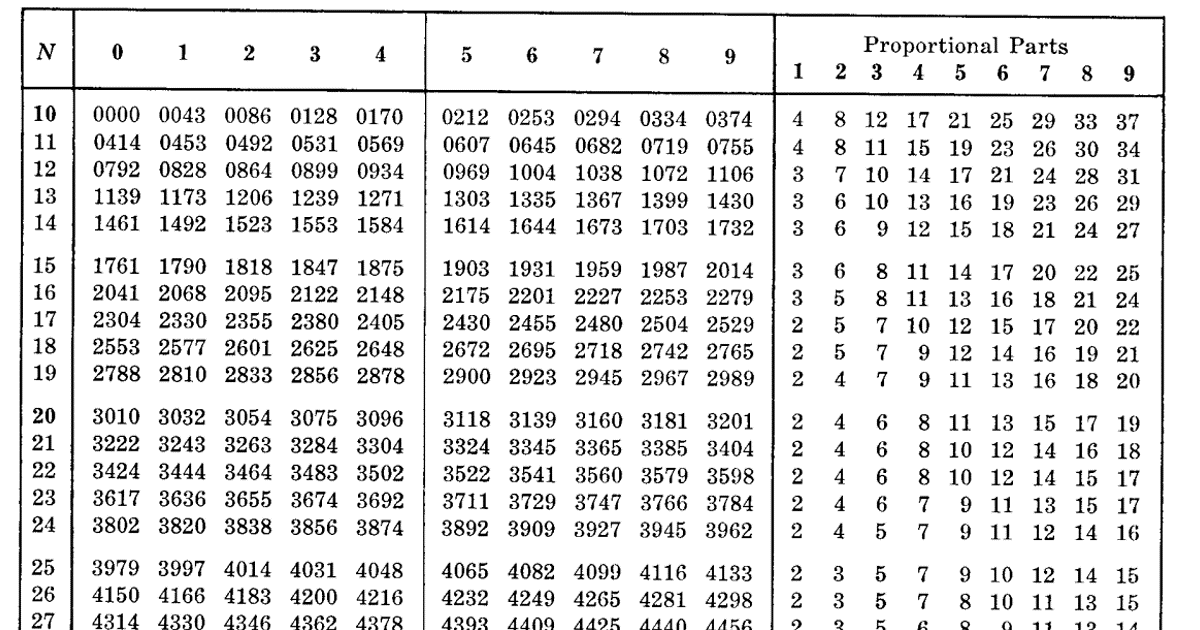
\includegraphics[width=0.7\textwidth]{tu/logarithm_table2.png}
    \caption*{\texttt{一份对数表，可以看到$25$对应$1.3979$}}
\end{figure}

那么$a$是多少呢？首先我们把$25$写成$2.5\times 10$。只要找出$2.5$对应的数$b$，就有$a = b+1$。$2.5$对应什么数呢？天文学家为此编了一张表，以$0.001$为单位，把$1$到$10$之间的数对应的数都列了出来，叫做\textbf{对数表}。查对数表\footnote{关于对数表及其使用方法，参见附录A：常用对数表。}可知，$2.5$对应的数$b = 0.3979$。因此$25$对应的数为$1.3979$。我们把$1.3979$称为$25$的\textbf{对数}，把$25$称为$1.3979$的\textbf{真数}。
$$ 25 \approx 10^{1.3979}.$$

用这个方法，我们可以把所有的数都转换成$10$的乘方，把所有乘除法都换成加减法。比如计算织女星半径：
\begin{align*}
    R &= \frac{d}{T^2}\sqrt{\frac{F}{\sigma}} = \frac{25\times 9\dlim{4607}\dlim{3047}\dlim{2580}.8}{9300^2} \times \sqrt{\frac{0.03}{0.0567}} \\
    &\approx \frac{10^{1.3979}\times 10^{12.9759}}{10^{3.9685\times 2}} \times \sqrt{\frac{10^{-1.5229}}{10^{-1.2464}}} \\
    &\approx 10^{1.3979 + 12.9759 - 3.9685\times 2 + \frac{(-1.5229) - (-1.2464)}{2}}\\
    &= 10^{6.2985} \approx 1.988\times 10^6 = 198\dlim{8000} \; \mbox{（公里）}
\end{align*}

最后一步我们把$10^{6.2985}$写成$10^{0.2985}\times 10^{6}$，然后反查表找到$0.2985$对应的真数为$1.988$。于是$10^{6.2985}$转换为$1.988\times 10^6$。如果我们只想知道织女星的半径大概有多大，甚至可以看着$6.2985$说：大概比$10$的$6$次方公里大一些，也就是数百万公里。可以看到，通过查对数的方式，我们可以方便地计算大数的乘除法，估计结果的大小。这种估算方法叫做\textbf{对数法}。

我们可以把用对数法估算大数乘除法归纳为：
\begin{center}
    \fbox{
        \shortstack[l]{
            1. 将所有数转为科学记法。\\
            2. 查表将所有尾数转为其对数。\\
            3. 把尾数的对数和量级相加，作为指数。\\
            4. 把原式的乘法改为加法，除法改为减法，\\
            \phantom{4. }乘方改为乘法，开方改为除法。计算指数。\\
            5. 把计算结果的整数部分作为量级$n$。\\
            6. 反查表找出结果的小数部分对应的真数$A$。\\
            \phantom{4. }$A\times 10^n$就是估算结果。
        }
    }
\end{center}

\clearpage

\begin{sk}
    \mbox{}\\
    \indent 1. 天文学家为什么用$10$的乘方来表示真数？能不能用别的数代替$10$？\\
    \indent 2. 每个真数都有自己的对数吗？为什么？
\end{sk}

\chapter{二次方根和二次根式}
分式开平方得到的代数式，叫做\textbf{二次根式}。二次根式可以看成用代数式代替二次方根$\sqrt{q}$中的数量$q$得到的结果。
$\sqrt{c}$、$\sqrt{1 - a + a^2}$、$\sqrt{x^3 - x^2 - 2}$等都是二次根式。通过二次根式，我们可以更好地理解二次方根的性质。

\section{二次方根的化简}
\begin{sk}\label{sk:3-0-0}
    以下二次方根有什么联系？\\
    \indent 1. $\sqrt{2}$、$\sqrt{8}$、$\sqrt{72}$.\\
    \indent 2. $\sqrt{3}$、$\sqrt{45}$、$\sqrt{147}$.\\
    \indent 3. $\sqrt{5}$、$\sqrt{\frac{5}{4}}$、$\sqrt{\frac{20}{49}}$.
\end{sk}
如果正整数$n$有完全平方数$a^2$作为因数\footnote{其中$a>1$，下同。}：$n = ma^2$，那么
$$\sqrt{n} = \sqrt{m}\sqrt{a^2} = a\sqrt{m}.$$
用这个方法，可以把正整数$n$的二次方根$\sqrt{n}$写成一个整数$a$和一个无理数$\sqrt{m}$的乘积。其中$m$没有完全平方数作为因数，
所以$\sqrt{m}$是无理数。我们把这样的形式称为$\sqrt{n}$的\textbf{最简形式}，把找到最简形式的过程称为
（整数）二次方根的化简。

要化简整数的二次方根，可以先把整数分解成素因数的乘积。给定（大于$1$的）正整数$n$，写出它的标准分解：
$$n = p_1^{u_1} p_2^{u_2} \cdots p_k^{u_k}$$
如果某个素因数$p_i$在$n$中的指数$u_i$是偶数，那么$p_i^{u_i}$是一个完全平方数；
如果$u_i$是奇数，那么$p_i^{u_i-1}$是一个完全平方数。于是，我们可以把$n$的素因数分为两类，
一类是指数为偶数的，另一类是指数为奇数的。我们可以把前一类中的$p_i^{u_i}$和后一类的$p_i^{u_i-1}$提出来，
相乘得到一个完全平方数。剩下的就是指数为奇数的素因数的乘积。如果我们定义这样的函数：
$$ \varsigma: n = p_1^{u_1} p_2^{u_2} \cdots p_k^{u_k} \mapsto p_1^{r_1} p_2^{r_2} \cdots p_k^{r_k}. $$
其中的$r_1, r_2, \cdots r_k$分别是$u_1, u_2, \cdots u_k$除以$2$的余数。那么$\varsigma(n)$就是剩下的指数为奇数的素因数的乘积。
而$\frac{n}{\varsigma(n)}$是一个完全平方数。

$\varsigma(n)$已经没有完全平方数的因子了，我们把它叫做$n$的\textbf{二次方余}。$n$可以写成：
$$ \sqrt{n} = a\sqrt{\varsigma(n)}.$$
其中正整数$a$是$\frac{n}{\varsigma(n)}$的平方根。

举例来说，要化简$\sqrt{2520}$，可以先把正整数$2520$分解：
$$ 2520 = 2^3 \cdot 3^2 \cdot 5 \cdot 7.$$
然后提出完全平方的部分，计算方余：
$$ 2520 = \left(2^2 \cdot 3^2 \right) \cdot (2 \cdot 5 \cdot 7)$$
因此$\varsigma(n) = 2 \cdot 5 \cdot 7 = 70$，
$$ \sqrt{2520} = 6 \sqrt{70}.$$

对一般的正有理数$r$，我们也希望将$\sqrt{r}$表示成$a\sqrt{m}$的形式，其中$a$是有理数，
而$m$是没有完全平方数因子的正整数。我们把这样的形式称为有理数二次方根的最简形式。

把$r$写成既约分数：$r = \frac{p}{q}$，不难发现，可以把$\sqrt{r}$写成：
$$ \sqrt{r} = \sqrt{\frac{p}{q}} = \sqrt{\frac{pq}{q^2}} = \frac{\sqrt{pq}}{q}.$$
这样，只需要把正整数$pq$的二次方根化简，就能得到$\sqrt{r}$的最简形式。

对整式和分式来说，它们开平方得到的二次根式也可以用类似的方式化简。

\begin{sk}
    \mbox{} \\
    \indent 1. 设$k,n$是正整数，$k>2$。如何对$k$次方根$\sqrt[k]{n}$进行类似二次方根的化简？
\end{sk}

\begin{xt}\label{xt:3-0-0}
    \mbox{} \\
    \indent 1. 化简以下的二次方根：\\
    \indent 1.1. $\sqrt{5480}$、$\sqrt{1240}$、$\sqrt{5760}$.\\
    \indent 1.2. $\displaystyle\frac{2}{\sqrt{3}}$、$\displaystyle\sqrt{\frac{1744}{85}}$、$\displaystyle\sqrt{\frac{576}{132}}$、$\displaystyle\sqrt{\frac{2240}{6897}}$.\\
    \indent 1.3. $\sqrt{48} - 1.8\sqrt{6} + 5\sqrt{3}$、$7\sqrt{18} + 1.5\sqrt{108} + 10\sqrt{242}$.\\
    \indent 2. 化简以下的代数式：\\
    \indent 2.1. $\sqrt{a^3b}$、$\displaystyle\sqrt{\frac{a}{b^5}}$、$\sqrt{(1 - a^2)(1 + a)}$、$\sqrt{(b^3 - a^3)(b - a)}$.\\
    \indent 2.2. $\displaystyle\sqrt{\frac{1 - a^4}{(1 + a)^3}}$、$\displaystyle\sqrt{\frac{1 - a^4}{a(a+1)}} + \sqrt{a^2+1}$.
\end{xt}

\section{二次方根分式的化简}
一个或多个二次方根和有理数进行加减乘除运算的结果，称为\textbf{二次方根分式}。如果仅仅是二次方根和有理数进行加减乘运算的结果，就称为\textbf{二次方根整式}。

比如，$\displaystyle (1 - \sqrt{3})^2 + \sqrt{7}$、$\displaystyle \frac{(1+\sqrt{5})^2}{2}$、$\displaystyle \frac{2 - \sqrt{3}}{\sqrt{2} + 1}$、$\displaystyle \frac{(1 + \sqrt{5})^3 + 2\sqrt{6}}{2((\sqrt{3} - 1)^2 + 2\sqrt{2} - 5)}$等等都是二次方根分式。其中$\displaystyle (1 - \sqrt{3})^2 + \sqrt{7}$是二次方根整式。$\displaystyle \frac{(1+\sqrt{5})^2}{2}$是二次方根分式，但如果把分母的$2$视为乘以有理数$\frac{1}{2}$，那么也可以看作二次方根整式。

一般来说，我们认为二次方根分式，特别是分母中出现了二次方根的分式，比较复杂。把复杂的二次方根分式转化为二次方根整式，称为二次方根分式的化简。

二次方根整式相乘的结果总是二次方根整式。因此，如果能把二次方根整式的倒数转为二次方根整式，那么二次方根分式就能转为两个二次方根整式的乘积，从而转为二次方根整式。

首先来看一种简单的情况——分母是关于$\sqrt{n}$的一次式。这时二次方根分式可以写为：
$$ \frac{1}{a + b\sqrt{n}} ,$$
其中$a$是有理数，$b$是非零有理数，$n$是正整数且不是任何整数的平方。我们把分子分母各乘以$a - b\sqrt{n}$，得到：
$$ \frac{1}{a + b\sqrt{n}} = \frac{a - b\sqrt{n}}{(a + b\sqrt{n})(a - b\sqrt{n})} = \frac{a - b\sqrt{n}}{a^2 - (b\sqrt{n})^2} = \frac{a - b\sqrt{n}}{a^2 - nb^2}.$$
分母$a^2 - nb^2$是有理数，所以上式变成了一个二次方根整式：
$$ \frac{1}{a + b\sqrt{n}} = \frac{a - b\sqrt{n}}{a^2 - nb^2} = \frac{a}{a^2 - nb^2} - \frac{b}{a^2 - nb^2}\sqrt{n}.$$

这种方法是否总有效呢？有一个地方需要检查：$a - b\sqrt{n}$是否会是$0$。答案是否定的，$a - b\sqrt{n}$总不为$0$。下面用反证法证明。

反设$a - b\sqrt{n}=0$，那么$\displaystyle\sqrt{n} = \frac{a}{b}$是有理数。将它约分，写成既约分数：$\displaystyle\sqrt{n} = \frac{p}{q}$，则：
$$ p^2 = q^2n.$$
考虑正整数$p$的标准分解。设$p_1$是$p$的某个素因数，那么$p_1$不是$q$的素因数，因而$p_1$只能是$n$的素因数。以此类推，$p$的所有素因数都是$n$的素因数。设$p_1$在$p$的标准分解里的次数是$u_1$，在$n$的标准分解里的次数是$v_1$，则$2u_1=v_1$。这说明$p^2 = n$，$q=1$，于是$n$是完全平方数，矛盾！这说明原命题的否定“$a - b\sqrt{n}=0$”是假的。所以$a - b\sqrt{n}$总不为$0$。也就是说，我们总有：
$$ \frac{1}{a + b\sqrt{n}} = \frac{a}{a^2 - nb^2} - \frac{b}{a^2 - nb^2}\sqrt{n}.$$

考虑更一般的情况——所有方根都相同的二次方根分式：
$$ Q = \frac{a_0 + a_1\sqrt{n} + \cdots + a_l \sqrt{n}^l}{b_0 + b_1\sqrt{n} + \cdots + b_m \sqrt{n}^m}, $$
其中$l,m$是正整数，$n$是正整数但不是完全平方数。$a_0, a_1, \cdots, a_l, b_0, b_1,\cdots b_m$是有理数。这样的二次方根分式如何化简呢？

为了好说话，我们把作为位于分子和分母的整式分别称为分子式和分母式。我们先分别化简分子式和分母式。$\sqrt{n}$的平方是整数$n$，所以可以把分子式（分母式）看作关于$\sqrt{n}$的多项式。其中$\sqrt{n}$偶数次方的项可以看作关于$n$的有理数系数整式，所以它的值是有理数。$\sqrt{n}$奇数次方的项可以看作$\sqrt{n}$乘以$\sqrt{n}$的偶数次方，因此每一项都可以看作有理数乘以$\sqrt{n}$。合并同类项之后，无论分子式还是分母式都可以写成关于$\sqrt{n}$的一次有理数系数整式，也就是说：
$$ Q =  \frac{a_0' + a_1'\sqrt{n}}{b_0' + b_1'\sqrt{n}}, $$
其中$a_0', a_1', b_0' , b_1'$是有理数。
根据前面讨论过的简单情况下的结论，我们可以将它继续化简为：
\begin{align*}
    Q &=  (a_0' + a_1'\sqrt{n})\cdot \frac{1}{b_0' + b_1'\sqrt{n}} = (a_0' + a_1'\sqrt{n}) \left(\frac{b_0'}{b_0'^2 - nb_1'^2} - \frac{b_1'}{b_0'^2 - nb_1'^2}\sqrt{n}\right) \\
    &= \frac{a_0'b_0' - a_1'b_1'n}{b_0'^2 - nb_1'^2} + \left(\frac{a_1'b_0' - a_0'b_1'}{b_0'^2 - nb_1'^2}\right)\sqrt{n}.
\end{align*}
这说明所有方根都相同的二次方根分式总可以化简为关于$\sqrt{n}$的一次有理数系数整式，写成$a + b\sqrt{n}$的形式。

如果二次方根分式里有多个不同的二次方根，计算将更加复杂。从以上的化简过程来看，化简含有二次方根$\sqrt{n}$的式子，要把它看作关于$\sqrt{n}$的多项式$P(x)$在$x = \sqrt{n}$时的值。然后设法把$P(x)$表示成某个关于$x^2$的整式$R(x^2)$。$x^2 = n$是整数，所以$P(x) = R(x^2)$里就不再有$\sqrt{n}$了。

\begin{et}
    化简以下含有二次方根的式子：\\
    $$
    \begin{array}{lll}
       1).\;\; \displaystyle \frac{\sqrt{5} + 1}{3 - 2\sqrt{5}} &  \phantom{00000000} & 2).\;\; \displaystyle \frac{\sqrt{3} + 1}{6 - \sqrt{5}} \\[2em]
       3).\;\; \displaystyle \frac{(\sqrt{5} - 1)^2 + \sqrt{5} - 3}{(1 - 2\sqrt{5})^2 + 2\sqrt{5} - 17} &  \phantom{00000000} & 4).\;\; \displaystyle \frac{2\sqrt{3} - 3}{1 + \sqrt{2} + \sqrt{3}}
    \end{array}
    $$
\end{et}

\begin{so}
    \mbox{} \\
    \indent 1). 解：
    \begin{align*}
        \frac{\sqrt{5} + 1}{3 - 2\sqrt{5}} & = \frac{(\sqrt{5} + 1)(3 + 2\sqrt{5})}{(3 - 2\sqrt{5})(3 + 2\sqrt{5})} \\
        &= \frac{3 + 2\cdot 5 + 3\sqrt{5} + 2\sqrt{5}}{3^2 - 2^2\cdot 5} \\
        &= -\frac{13 + 5\sqrt{5}}{11} = -\frac{13}{11} - \frac{5}{11}\sqrt{5}
    \end{align*}
    
    \indent 2).  解：
    \begin{align*}
        \frac{\sqrt{3} + 1}{6 - \sqrt{5}} &= \frac{(\sqrt{3} + 1)(6 + \sqrt{5})}{(6 - \sqrt{5})(6 + \sqrt{5})} \\
        &= \frac{6 + 6\sqrt{3} + \sqrt{5} + \sqrt{15}}{6^2 - 5} = \frac{6 + 6\sqrt{3} + \sqrt{5} + \sqrt{15}}{31} \\
        &= \frac{6}{31} + \frac{6}{31}\sqrt{3} + \frac{1}{31}\sqrt{5} + \frac{1}{31}\sqrt{15}
    \end{align*}

    \indent 3).  解：
    \begin{align*}
        &\; \frac{(\sqrt{5} - 1)^2 + \sqrt{5} - 3}{(1 - 2\sqrt{5})^2 + 2\sqrt{5} - 17} \\
        =&\; \frac{1 + 5 - 2\sqrt{5} + \sqrt{5} - 3}{1 + 2^2\cdot 5 - 4\sqrt{5} + 2\sqrt{5} - 17} \\
        =&\; \frac{3 - \sqrt{5}}{4 - 2\sqrt{5}} \\
        =&\; \frac{(3 - \sqrt{5})(2 + \sqrt{5})}{2(2 - \sqrt{5})(2 + \sqrt{5})} \\
        =&\; \frac{3\cdot 2 - 5 - 2\sqrt{5} + 3\sqrt{5}}{2(2^2 - 5)} \\
        =&\; -\frac{1 + \sqrt{5}}{2} = -\frac{1}{2} - \frac{1}{2}\sqrt{5}\\
    \end{align*}

    \indent 4). 解：
    \begin{align*}
        \frac{2\sqrt{3} - 3}{1 + \sqrt{2} + \sqrt{3}} &= \frac{(2\sqrt{3} - 3)(1 - \sqrt{2} + \sqrt{3})}{(1 + \sqrt{2} + \sqrt{3})(1 - \sqrt{2} + \sqrt{3})} \\
        &= \frac{-3 + 2 \cdot 3 + 2\sqrt{3} - 2\sqrt{6} + 3\sqrt{2} - 3\sqrt{3}}{(1 + \sqrt{3})^2 - 2} \\
        &= \frac{3 + 3\sqrt{2} - \sqrt{3} - 2\sqrt{6}}{1 + 3 + 2\sqrt{3} - 2} = \frac{3 + 3\sqrt{2} - \sqrt{3} - 2\sqrt{6}}{2 + 2\sqrt{3}} \\
        &= \frac{(3 + 3\sqrt{2} - \sqrt{3} - 2\sqrt{6})(1 - \sqrt{3})}{2(1 + \sqrt{3})(1 - \sqrt{3})} \\
        &= \frac{3 + 3\sqrt{2} - \sqrt{3} - 2\sqrt{6} - 3\sqrt{3} - 3\sqrt{6} + 3 + 2\cdot 3\sqrt{2}}{2(1^2 - 3)} \\
        &= -\frac{6 + 9\sqrt{2} - 4\sqrt{3} - 5\sqrt{6}}{4} = -\frac{3}{2} - \frac{9}{4}\sqrt{2} + \sqrt{3} + \frac{5}{4}\sqrt{6}\\
    \end{align*}
\end{so}

\begin{sk}
    \mbox{} \\
    \indent 1. 例题$4$中，为什么分子和分母要分别乘以$1 - \sqrt{2} + \sqrt{3}$？还有什么别的方法化简吗？\\
    \indent 2. 如果分母式是关于$k$次方根的整式$a + b\sqrt[k]{n}$，如何化简？
    % \indent 3. 
\end{sk}

\begin{xt}
    \mbox{} \\
    \indent 1. 化简以下含有二次方根的式子：\\
    $$
    \begin{array}{lll}
       1).\;\; \displaystyle \frac{1 - \sqrt{2}}{1 + 2\sqrt{2}} &  \phantom{00000000} & 2).\;\; \displaystyle \frac{\sqrt{2} - \sqrt{3} + 1}{2 - \sqrt{2}} \\[2em]
       3).\;\; \displaystyle \frac{(\sqrt{3} - 2)^2 + 2\sqrt{3} - 3}{(1 + \sqrt{3})^2 + 2\sqrt{3} - 7} &  \phantom{00000000} & 4).\;\; \displaystyle \frac{1 + 2\sqrt{5}}{2 + \sqrt{2} - \sqrt{5}}
    \end{array}
    $$
    \indent 2. 设$n$是正整数，考虑$(1 + \sqrt{2})^n$。\\
    \indent 2.1. 证明：$(1 + \sqrt{2})^n$总可以写成$(1 + \sqrt{2})^n = a_n + b_n \sqrt{2}$
    的形式。\\
    \indent \phantom{2.1.} 其中$a_n, b_n$是正整数。\\
    \indent 2.2. 当$n=1,2,3,4$时，写出对应的$a_n$和$b_n$。\\
    \indent 2.3. 给定正整数$n$，用$a_n$和$b_n$表示$a_{n+1}$和$b_{n+1}$。\\
    \indent 2.4. 用归纳法证明：
    $$\forall n, \quad (1 - \sqrt{2})^n = a_n - b_n \sqrt{2}.$$ 
    \indent 2.5. 证明：对任意正整数$n$，总有$a_{n+2} = 2a_{n+1} + a_n$。\\
    % \begin{align*}
    %     a_{n+1} + b_{n+1} \sqrt{2} &= (a_n + b_n \sqrt{2})(1 + \sqrt{2})\\
    %     &= a_n + 2b_n + (a_n + b_n)\sqrt{2}
    %     a_{n+1} &= a_n + 2b_n \\
    %     b_{n+1} &= a_n + b_n \\
    %     a_{n} &= \frac{(1 + \sqrt{2})^n + (1 - \sqrt{2})^n}{2} \\
    %     a_{n+2} - 2a_{n+1} - a_n &= 0 \\
    %     a_{n+2} &= a_{n+1} + 2b_{n+1} = a_{n+1} + 2a_n + 2b_n = 2a_{n+1} + a_n \\
    % \end{align*}
    \indent 2.6. 用归纳法证明：对任意正整数$n$，$a_{2n} + a_{2n+1}$总是$4$的倍数；\\
    \indent \phantom{2.1.} $a_{3n+1} + a_{3n+2} + a_{3n+3}$总是$5$的倍数。

\end{xt}

\sectionext{二次域}
上一节中我们看到，所有关于同一个二次方根$\sqrt{n}$的分式，都能化简为$a + b\sqrt{n}$的形式。这让我们想要考察形如$a + b\sqrt{n}$的数的集合。

考虑这样一个集合：$\{a + b\sqrt{2} \, | \, a, b \in\mathbb{Q}\}$。有理数集$\mathbb{Q}$是它的子集，
它是实数集$\mathbb{R}$的子集。我们把它记为$\mathbb{Q}(\sqrt{2})$。

举例来说，$\mathbb{Q}(\sqrt{2})$的元素有：$1 + \sqrt{2}$、$3 - 2\sqrt{2}$、$0$、$-7.2$等等。

$\mathbb{Q}(\sqrt{2})$的元素有什么性质呢？

$1 + \sqrt{2}$和$3 - 2\sqrt{2}$是$\mathbb{Q}(\sqrt{2})$的元素，它们的和是$4 - \sqrt{2}$，
差是$-2 + 3\sqrt{2}$，乘积是$-1 + \sqrt{2}$，商是$7 + 5\sqrt{2}$。

一般来说，如果$x$和$y$是$\mathbb{Q}(\sqrt{2})$的元素，它们进行四则运算的结果仍然是$\mathbb{Q}(\sqrt{2})$的元素。具有这种性质的数集叫做\textbf{数域}。有理数、实数都是数域，自然数、整数、正数不是数域。
$\mathbb{Q}(\sqrt{2})$、$\mathbb{Q}(\sqrt{3})$这样的数域叫做\textbf{二次域}。

如果$n$是正整数，$\sqrt{n}$在不在$\mathbb{Q}(\sqrt{2})$里呢？
\begin{tm}
    $\sqrt{3}$不属于$\mathbb{Q}(\sqrt{2})$。
\end{tm}\label{tm:3-1-0}
\begin{proof}
    用反证法。反设$\sqrt{3}$属于$\mathbb{Q}(\sqrt{2})$。于是存在有理数$a,b$使得
    $$ \sqrt{3} = a + b\sqrt{2}.$$
    两边平方，得到：
    $$ 3 = a^2 + 2b^2 + 2ab\sqrt{2}.$$
    如果$ab \neq 0$，那么$ \sqrt{2} = \frac{3 - a^2 - 2b^2}{2ab}$是有理数。矛盾！\\
    如果$a = 0$，那么$2b^2 = 3$，于是$b = \frac{\sqrt{6}}{2}$是无理数。矛盾！\\
    如果$b = 0$，那么$a^2 = 3$，于是$a = \sqrt{3}$是无理数。矛盾！\\
    综上所述，原命题的否定“$\sqrt{3}$属于$\mathbb{Q}(\sqrt{2})$”是假的，因此原命题是真的。
\end{proof}

用同样的方法，可以证明$\sqrt{2}$不属于$\mathbb{Q}(\sqrt{3})$。也就是说，$\mathbb{Q}(\sqrt{2})$
不是$\mathbb{Q}(\sqrt{3})$的子集，$\mathbb{Q}(\sqrt{3})$也不是$\mathbb{Q}(\sqrt{2})$的子集。这说明$\mathbb{Q}(\sqrt{2})$和$\mathbb{Q}(\sqrt{3})$的交集是$\mathbb{Q}$。

\begin{sk}\label{sk:3-2-0}
    \mbox{}\\
    \indent 1. 对哪些正整数$n$，$\sqrt{n}$在$\mathbb{Q}(\sqrt{2})$里？\\
    \indent 3. $\mathbb{Q}(\sqrt{2})$和$\mathbb{Q}(\sqrt{3})$的并集是什么集合？是不是数域？
\end{sk}

\begin{xt}\label{xt:3-2-0}
    \mbox{}\\
    \indent 1. 证明：$\mathbb{Q}(\sqrt{2})$和$\mathbb{Q}(\sqrt{3})$的交集是$\mathbb{Q}$。\\
    \indent 2. 记$x = \sqrt{1 + \sqrt{2}}$。\\
    \indent 2.1. 假设有$a,b\in\mathbb{Q}$使得$x = a + b\sqrt{2}$。证明：$a^2 + 2b^2 = 1 = 2ab$。\\
    % \begin{align*}
    %     1 + \sqrt{2} = x^2 = (a + b\sqrt{2})^2 = a^2 + 2b^2 + 2ab\sqrt{2} \\
    % \end{align*}
    \indent 2.2. 由此说明$x$不是二次域$\mathbb{Q}(\sqrt{2})$的元素\footnote{提示：考虑$a^2 - 2ab + 2b^2$。}。
\end{xt}

\chapter{一元二次方程}
我们已经学习过一元一次方程。解一元一次方程可以看作找出一元一次式$ax + b$等于$0$时变量$x$的值。
找出一元二次式$ax^2 + bx + c$等于$0$时$x$的值，叫做解一元二次方程。

\begin{ex}\label{ex:4-0-0}
    根据以下问题，设未知数并列出方程：\\
    $(1).$ 一座方城，南北正中有城门。北门出城直走$100$步有树，南门出城直走$100$步转西，走$1200$步后恰能望到。问方城长度是多少？\\
    $(2).$ 氢气和碘蒸气产生化学反应：
    $$\mathrm{H}_2 + \mathrm{I}_2 \longrightarrow 2\mathrm{HI}$$
    $50$摄氏度时，正反应的平衡常数$k_c=5.25$。
    现在将$1$摩尔氢气和$2$摩尔碘蒸气放置于$1$升的容器中，将温度调节到$50$摄氏度。反应达到平衡时，
    有多少摩尔的$HI$产生？
\end{ex}

\begin{so}
    \mbox{} \\
    $(1)$解：设方城长$x$步，北门位置为$M$点，外树的位置为$A$点，南门外转向的位置为$B$点，
    西行恰好望见树的位置为$C$点，城西北角为$N$点。直角三角形$AMN$和$ABC$相似。因此：
    $$ \frac{|AM|}{|MN|} = \frac{|AB|}{|BC|} $$
    根据已知条件，$|AM| = 100$，$|MN| = 0.5x$，$|AB| = x + 200$，$|BC| = 1200$。于是可以列出方程：
    $$ \frac{100}{0.5x} = \frac{x + 200}{1200}, $$
    即：
    \begin{align*}
        0.5x(x + 200) &= 100 \times 1200  \\
        x^2 + 200x &= 100 \times 1200 \div 0.5 = 240000  \\
        x^2 + 200x &- 240000 = 0  
    \end{align*} 

\noindent
\begin{tikzpicture}[scale=0.7]
    % 方城参数
    \pgfmathsetmacro{\citySize}{4}    % 方城边长
    \pgfmathsetmacro{\treeNorth}{1}   % 北门出城100步
    \pgfmathsetmacro{\walkSouth}{1}   % 南门出城100步
    \pgfmathsetmacro{\walkWest}{12}    % 西行1200步
    \pgfmathsetmacro{\door}{0.24}    % 城门用

    % 绘制坐标轴
    \draw[->] (-12.8,0) -- (3,0) node[below right] {$x\;(\mbox{\texttt{每}}100\mbox{\texttt{步}})$};
    \draw[->] (0,-3.5) -- (0,4.8) node[below right] {$y\;(\mbox{\texttt{每}}100\mbox{\texttt{步}})$};

    \foreach \x in {-12,...,-1} {
        \draw (\x,0) -- (\x,-0.1);
        \node [below] at (\x,0) {\x};
    }
    
    \foreach \x in {1,2} {
        \draw (\x,0) -- (\x,-0.1);
        \node [below] at (\x,0) {\x};
    }

    \foreach \y in {-3,...,-1} {
        \draw (0,\y) -- (-0.1,\y);
        \node [left] at (0,\y) {\y};
    }

    \foreach \y in {1,...,4} {
        \draw (0,\y) -- (-0.1,\y);
        \node [left] at (0,\y) {\y};
    }

    % 绘制方城（以原点为中心）
    \draw[very thick, draw=Sepia] (-\citySize/2, -\citySize/2) rectangle (\citySize/2, \citySize/2);
    \draw[thick, draw=Sepia] (-\door/2, \citySize/2) -- (-\door/2, \citySize/2 + \door/2);
    \draw[thick, draw=Sepia] (\door/2, \citySize/2) -- (\door/2, \citySize/2 + \door/2);
    \draw[thick, draw=Sepia] (-\door/2, -\citySize/2) -- (-\door/2, -\citySize/2 - \door/2);
    \draw[thick, draw=Sepia] (\door/2, -\citySize/2) -- (\door/2, -\citySize/2 - \door/2);
    \draw[thick, draw=Sepia] (\citySize/2, -\door/2) -- (\citySize/2 + \door/2, -\door/2);
    \draw[thick, draw=Sepia] (\citySize/2, \door/2) -- (\citySize/2 + \door/2, \door/2);
    \draw[thick, draw=Sepia] (-\citySize/2, -\door/2) -- (-\citySize/2 - \door/2, -\door/2);
    \draw[thick, draw=Sepia] (-\citySize/2, \door/2) -- (-\citySize/2 - \door/2, \door/2);
    
    % 绘制树
    \node[draw, circle, fill=green!50!black, inner sep=2pt] at (0, \citySize/2 + \treeNorth) {};
    \node[above] at (0, \citySize/2 + \treeNorth) {};
    
    % 绘制南门出城路径
    \draw[-{Latex[length=2.5mm,width=2mm]}, thick, draw=red] (0, \citySize/2) -- node[right] {\texttt{北门出城直走}$100$\texttt{步}}  (0, \citySize/2 + \walkSouth);
    \draw[thick, draw=red] (0, -\citySize/2) -- (0, -\citySize/2 - \walkSouth);
    \draw[-{Latex[length=2.5mm,width=2mm]}, thick, draw=red] (0, -\citySize/2 - \walkSouth) -- node[above] {\phantom{000}\texttt{南门出城直走}$100$\texttt{步转西走}$1200$\texttt{步}} (-\walkWest, -\citySize/2 - \walkSouth);
    
    % 绘制视角线
    \draw[dashed] (0, \citySize/2 + \treeNorth) -- (-\walkWest, -\citySize/2 - \walkSouth);

    \draw[-{Stealth[length=6mm,width=3mm]}, thick] (-10,3) -- (-10, 3.5);
    \draw[thick](-10, 3.05) circle (0.36);
    \node[above] at (-10, 3.5) {\texttt{北}};
    
\end{tikzpicture}

    $(2)$解：设平衡时产生了$x$摩尔的$HI$。根据反应方程式，这时$H_2$和$I_2$分别消耗了$0.5x$摩尔。
    因此平衡时三者浓度分别为$1 - 0.5x$摩尔/升、$2 - 0.5x$摩尔/升和$x$摩尔/升。根据条件，反应平衡常数为$5.25$，即浓度比：
    $$ \frac{(1 - 0.5x)(2 - 0.5x)}{x^2} = 5.25,$$
    也即：
    \begin{align*}
        5.25 x^2 = \left(1 - 0.5x\right)\left(2 - 0.5x\right) &= 0.25x^2 - (1 \cdot 0.5 + 2\cdot 0.5)x + 2 \\
        5x^2 + 1.5 x - 2 &= 0\\
        10 x^2 + 3x - 4 &= 0 
    \end{align*} 
\end{so}

\section{解一元二次方程}
怎么求一元二次方程的解呢？我们其实已经解决过一种简单的情形。
考虑等腰直角三角形，如果直角边长度为$1$，那么斜边长$x$满足：
$$x^2 = 2.$$
这就是个一元二次方程。解这个一元二次方程的方法是对右边的$2$开平方，得到解：
$$ x = \sqrt{2}.$$
当然，另一个解：$x = -\sqrt{2}$也满足方程。只是我们要求的斜边长度是正数，
所以这个解不是我们要找的。不过，仅就方程$ x^2 = 2$来说，它有两个解，
分别是$x_1 = \sqrt{2}$和$x_2 = -\sqrt{2}$。为了方便，有时我们也写成$x_{1,2} = \pm\sqrt{2}$。

$x^2 = 2$和一般的一元二次方程$ax^2 + bx + c = 0$有什么不同呢？我们注意到，
二次项$x^2$的系数不再是$1$，而且多了一次项$bx$。二次项系数的问题不难解决，
我们把方程两边同时除以$a$，就可以让二次项系数等于$1$：
$$ x^2 + \frac{b}{a} x + \frac{c}{a} = 0$$
至于一次项，我们希望通过一些手段把它“去掉”。这样，问题就转化为类似$x^2 = 2$的简单情形了。

第一种手段叫作配方法。我们希望把$x^2 + \frac{b}{a}x + \frac{c}{a}$表示与$x$相关的平方形式。观察平方和公式：
\begin{align*}
    (x + 1)^2 = x^2 + 2\cdot 1\cdot x + 1^2  \\
    (x + 2)^2 = x^2 + 2\cdot 2\cdot x + 2^2  \\
    (x + 3)^2 = x^2 + 2\cdot 3\cdot x + 3^2  \\
    \cdots 
\end{align*}
对任何数$t$，根据平方和公式，$(x + t)^2 = x^2 + 2tx + t^2$，如果让$2t = \frac{b}{a}$，
那么$(x + t)^2$就和$x^2 + \frac{b}{a}x + \frac{c}{a}$有相同的一次项了。
这时，$t = \frac{b}{2a}$，$(x + \frac{b}{2a})^2$展开得到$x^2 + \frac{b}{a}x + \frac{b^2}{4a^2} $，
和$x^2 + \frac{b}{a}x + \frac{c}{a}$还相差：$\frac{c}{a} - \frac{b^2}{4a^2}$。于是，原方程变成：
$$ \left(x + \frac{b}{2a}\right)^2 = \frac{b^2}{4a^2} - \frac{c}{a} = \frac{b^2 - 4ac}{4a^2}.$$
现在方程和$x^2 = 2$已经很像了。最后需要讨论等号右边常数项是否小于$0$。
实数$x + \frac{b}{2a}$的平方总大于等于$0$，所以，如果等号右边的常数项小于$0$，那么方程无解。
如果常数项恰好等于$0$，那么方程恰有一个解：$x = -\frac{b}{2a}$。如果常数项大于$0$，
那么方程和$x^2 = 2$一样有两个解。

第二种手段是待定系数法。我们可以直接猜测：$x^2 + \frac{b}{a} x + \frac{c}{a} = 0$能够写成
$(x - \lambda)^2 = \mu$的形式。把后者展开，通过对比各项系数，可以得到：$\lambda = -\frac{b}{2a}$，
$\mu = \frac{b^2 - 4ac}{4a^2}$。

无论哪一种方法，我们都发现，常数项$\frac{b^2 - 4ac}{4a^2}$的正负性质和方程解的个数有直接关系。
它的分母$4a^2$总是正数，所以关键在于分子：$b^2 - 4ac$。
我们把这个式子叫作一元二次方程$ax^2 + bx + c = 0$的\textbf{判别式}，记作$\Delta$：
$$\Delta = b^2 - 4ac.$$
$\Delta<0$时，方程无解；$\Delta = 0$时，方程有唯一解：$x = -\frac{b}{2a}$；$\Delta>0$时，方程有两个解：
$$x_{1,2} = \frac{-b \pm \sqrt{\Delta}}{2a}.$$
对二次整式$ax^2 + bx + c$来说，使得它等于$0$的$x$的值叫作它的根。$\Delta<0$时，整式无根；$\Delta>0$时，
整式有两个根。$\Delta = 0$时，整式变为$(x + \frac{b}{2a})^2$，我们说整式有二重根，或者说根的重数是$2$。
为了方便，对整式对应的方程，我们也使用“方程的根”的说法。这时，方程的根就是对应整式的根。

于是，我们可以给出上面两个例题中方程的解：
\begin{so}
    $1.$解：方程$ x^2 + 200x - 240000 = 0$的判别式是：
    $\Delta = 200^2 - 4\cdot 1\cdot (-240000) = 1000000 > 0$，所以方程有两个根：
    \begin{align*}
        x_{1,2} &= \frac{-200 \pm \sqrt{1000000}}{2\cdot 1}  \\
        &= \frac{-200 \pm 1000}{2} 
    \end{align*}

    即$x_1 = 400$和$x_2 = -600$。根据题目条件，$x>0$，所以解为$x = 400$。\\
    答：方城长$400$步。\\
    $2.$解：方程$10x^2 + 3x - 4 = 0$的判别式是：$\Delta = 3^2 - 4\cdot 10\cdot (-4) = 169 > 0$，
    所以方程有两个根：
    \begin{align*}
        x_{1,2} &= \frac{-3 \pm \sqrt{169}}{2\cdot 10}  \\
        &= \frac{-3 \pm 13}{20} 
    \end{align*}
    即$x_1 = 0.5$和$x_2 = -0.8$。根据题目条件，$x\geqslant 0$，所以解为$x = 0.5$。\\
    答：生成了$0.5$摩尔的$HI$。
\end{so}

\section{根和系数的关系}

上一节我们给出了一元二次方程$ax^2 + bx + c = 0$的解。
从根的角度，$ax^2 + bx + c $要么无根，要么有两个根。这两个根和变量的系数有什么关系呢？

写出两个根的表达式：
$$x_{1} = \frac{-b + \sqrt{\Delta}}{2a},\quad x_{2} = \frac{-b - \sqrt{\Delta}}{2a}.$$
要注意的是，从根的角度，$\Delta = 0$时，这个式子也成立。把两个根相加，得到：
$$ x_1 + x_2 = -\frac{b}{a}.$$
把它们相乘，得到：
$$ x_1 \cdot x_2 = \frac{c}{a}.$$
于是，
$$a(x - x_1)(x - x_2) = ax^2 - a(x_1 + x_2)x + ax_1x_2 = ax^2 + bx+c.$$
我们把$a(x - x_1)(x - x_2)$称为整式$ax^2 + bx+c$的根形式。

从另一个角度，可以这么理解：整式$ax^2 + bx + c$有两个根$x_1$和$x_2$，说明$x - x_1$和$x - x_2$都是它的因式。
$x_1 \neq x_2$时，$x - x_1$和$x - x_2$互素，于是$ax^2 + bx + c = (x - x_1)(x-x_2)q$，其中$q$是整式。
显然，如果$q$的次数大于$0$，$(x - x_1)(x-x_2)q$的次数就大于$2$了，因此$q$是常式。对比系数可知，$q = a$，
于是可以得出$ax^2 + bx+c$的根形式。

$x_1 = x_2$的时候，就无法直接得出$ax^2 + bx + c = (x - x_1)(x-x_2)q$了，所以需要特别指出根的重数是$2$，
它表示$ax^2 + bx + c = (x - x_1)^2 q$。这就是根的重数的用处。

设一元二次方程$ax^2 + bx + c$的系数是有理数。它的解$x_1$和$x_2$都是开方得到的，可能不是有理数，
而属于某个二次域。但它们的和与积是方程系数的商，所以必然是有理数。除此之外，如果计算其他关于$x_1$和$x_2$的式子，
结果可能就不是有理数了。比如，计算$x_1 - x_2$，可以得到：
$$ x_1 - x_2 = \frac{\sqrt{\Delta}}{a}. $$
$\frac{\sqrt{\Delta}}{a}$中有开方运算，不一定是有理数。

$x_1 - x_2$和$x_1 + x_2$、$x_1x_2$有什么区别呢？如果交换$x_1$和$x_2$的位置，$x_1 - x_2$会变成$x_2 - x_1$，
而$x_1 + x_2$、$x_1x_2$和原来一样。我们把交换$x_1$和$x_2$的位置而不变的二元整式叫作二元对称式。
二元对称式除了$x_1 + x_2$、$x_1x_2$还有很多，比如$x_1^2 + x_2^2$、$x_1x_2^2 + x_2x_1^2$等等。

一元二次方程的根是无理数的时候，有什么性质呢？先来看一个具体的例子。设有方程：$x^2 - 2x - 1 = 0$。它的根是：

$$ x_1 = 1 + \sqrt{2}, \quad x_2 = 1 - \sqrt{2}.$$

两个根都能写成$u + v\sqrt{2}$的形式（$u,v$是有理数）。也就是说，它们都是二次域$\mathbb{Q}(\sqrt{2})$的元素。
% 把两个根的有理系数和二次系数对应到直角坐标系里，分别对应点$(1, 1)$和$(1, -1)$。这两个点关于$x$轴对称，也关于点$-\frac{b}{2a}$对称。
一般情况：一元二次方程$ax^2 + bx + c$的系数是有理数，如果它有两个无理数解：
$$x_{1} = \frac{-b + \sqrt{\Delta}}{2a},\quad x_{2} = \frac{-b - \sqrt{\Delta}}{2a}.$$
设二次方根$\sqrt{\Delta}$化简的结果是：$\sqrt{\Delta} = r\sqrt{m}$，
那么两个根都是$\mathbb{Q}(\sqrt{m})$的元素。
% 把两个根的有理系数和二次系数对应到直角坐标系里，分别对应点$(-\frac{b}{2a}, \frac{r}{2a})$和$(-\frac{b}{2a}, -\frac{r}{2a})$。这两个点关于$x$轴对称，也关于点$-\frac{b}{2a}$对称。

如果直接把两个解放在数轴上看，它们也关于点$-\frac{b}{2a}$对称。如果把数轴看做$x$轴，建立直角坐标系，
那么两个解分别对应点$(x_1, \,\,0)$和$(x_2, \,\,0)$，它们关于直线$x = -\frac{b}{2a}$对称。

\chapter{函数初步（下）}
我们已经学习了正比例函数和一次函数。直角坐标系中，它们的图像是直线。
现在我们来看另外几种函数。

\section{反比例函数}
正比例函数是从正面描述比例关系的函数。除了正比例关系，我们还可以从另一个方面描述比例关系。
比如，两个三角形$\triangle ABC$和$\triangle A'B'C'$相似，那么
对应的边长成比例：
$$ \frac{|AB|}{|A'B'|} = \frac{|AC|}{|A'C'|} = \frac{|BC|}{|B'C'|} = k.$$
如果已知$|AB|$为定值，那么比例系数和$|A'B'|$的关系叫做反比例关系，对应的映射叫\textbf{反比例函数}。
一般来说，反比例函数是这样的：
$$ x \mapsto \frac{k}{x}$$
其中$k$是固定的系数。比如，$x \mapsto \frac{3}{x}$就是一个反比例函数。

反比例函数有什么性质呢？以$x \mapsto \frac{3}{x}$为例。下表是$x$取不同值时函数的值：

\begin{center}
    \begin{tabular}{| p{2em}<{\centering} | p{1.8em}<{\centering} | p{1.8em}<{\centering} | p{1.8em}<{\centering} | p{1.8em}<{\centering} | p{1.8em}<{\centering} | p{1.8em}<{\centering} | p{1.8em}<{\centering} | p{1.8em}<{\centering} | p{1.8em}<{\centering} |}
        \hline
        $x$ & -30 & -6 & -3 & -0.3 & 0.3 & 1 & 3 & 6 & 60 \\ [0.5ex] 
        \hline
        $f(x)$ & -0.1 & -0.5 & -1 & -10 & 10 & 3 & 1 & 0.5 & 0.05 \\   
        \hline
    \end{tabular}
\end{center}

对比$f(-0.3)$和$f(0.3)$、$f(-3)$和$f(3)$、$f(-6)$和$f(6)$，可以注意到：
如果$a$和$b$是相反数，那么$f(a)$和$f(b)$也是相反数。这个性质也可以写成：
$$ \forall x\in \mathbb{R}^*, \,\,\, f(-x) = -f(x).$$
这个性质可以用反比例函数的定义证明：
$$f(-x) = \frac{k}{-x} = -\frac{k}{x} = -f(x).$$

另外可以发现，$x<0$时，$f(x)$也小于$0$。$x$越小，$f(x)$越大。$x>0$时，$f(x)$也大于$0$。$x$越小，$f(x)$越大。
要注意的是，$x$不能等于$0$。反比例函数的定义域是不为零的实数的集合，记作$\mathbb{R}^*$或$\mathbb{R}^\times$。

把$3$换成其它的数，你有什么发现？

设有反比例函数$f: x \mapsto \frac{k}{x}$。当$k>0$的时候，$x$和$f(x)$同号。
$x<0$时，$x$的值越接近$0$，$f(x)$越小；$x>0$时，$x$的值越接近$0$，$f(x)$越大。
当$k<0$的时候，$x$和$f(x)$异号。
$x<0$时，$x$的值越接近$0$，$f(x)$越大；$x>0$时，$x$的值越接近$0$，$f(x)$越小。
$k$的正负对函数的性质有本质影响。

反比例函数的图像是怎样的呢？我们可以用描点法得到大致的模样，但目前我们掌握的知识，
还不足以严谨地勾画出反比例函数的图像。借助计算机作图软件，我们可以得到反比例函数的图像：

\begin{wrapfigure}[8]{r}{0.64\textwidth} %this figure will be at the right
    \vspace{-20pt}
    \flushright
    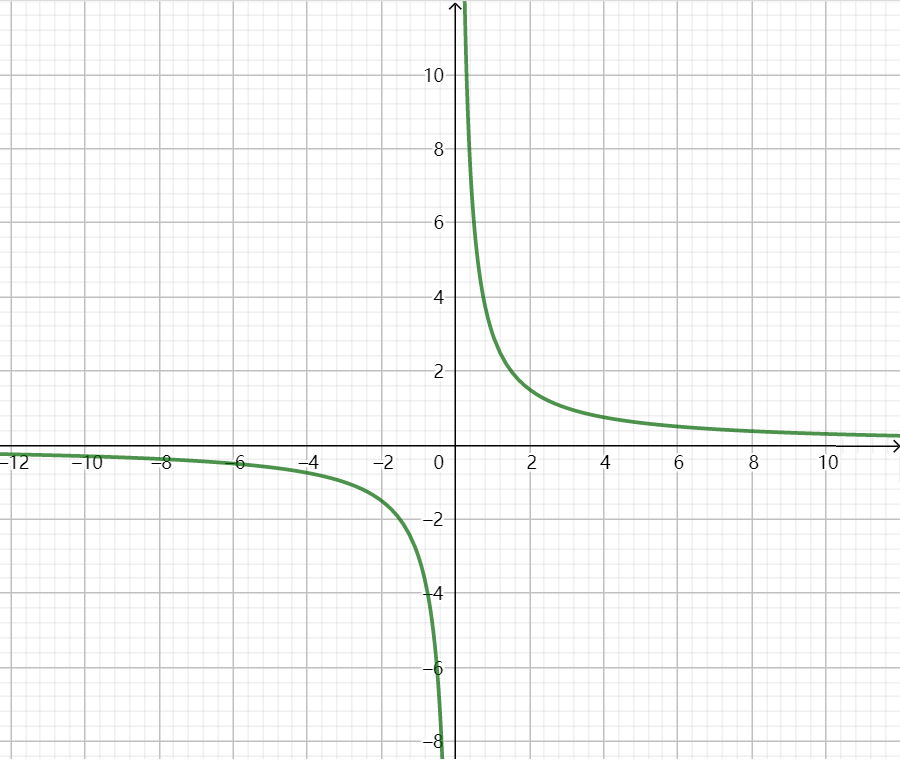
\includegraphics[width=0.6\textwidth]{tu/反比例函数1.png}
\end{wrapfigure}

我们说反比例函数的图像是一条曲线。右图中，第一象限中的部分叫做反比例函数的\textbf{正支}，
它是函数在$x>0$时的图像；第三象限中的部分叫做反比例函数的\textbf{负支}；它是函数在$x<0$时的图像。
$k>0$时，正支在第一象限，负支在第三象限；$k<0$时，正支在第四象限，负支在第二象限。

另外，反比例函数的图像关于原点中心对称。这可以通过性质：$f(-x) = -f(x)$得到。
对图像中每一点$(x, \,\,f(x))$，$(-x, \,\,-f(x)) = (-x, \,\,f(-x))$，因此它关于原点的对称点也在函数图像上。

对不同的$k$，反比例函数的图像有什么不一样呢？我们画出不同的$k$对应的反比例函数图像：

\begin{figure}[h] %this figure will be at the right
    % \vspace{-20pt}
    \centering
    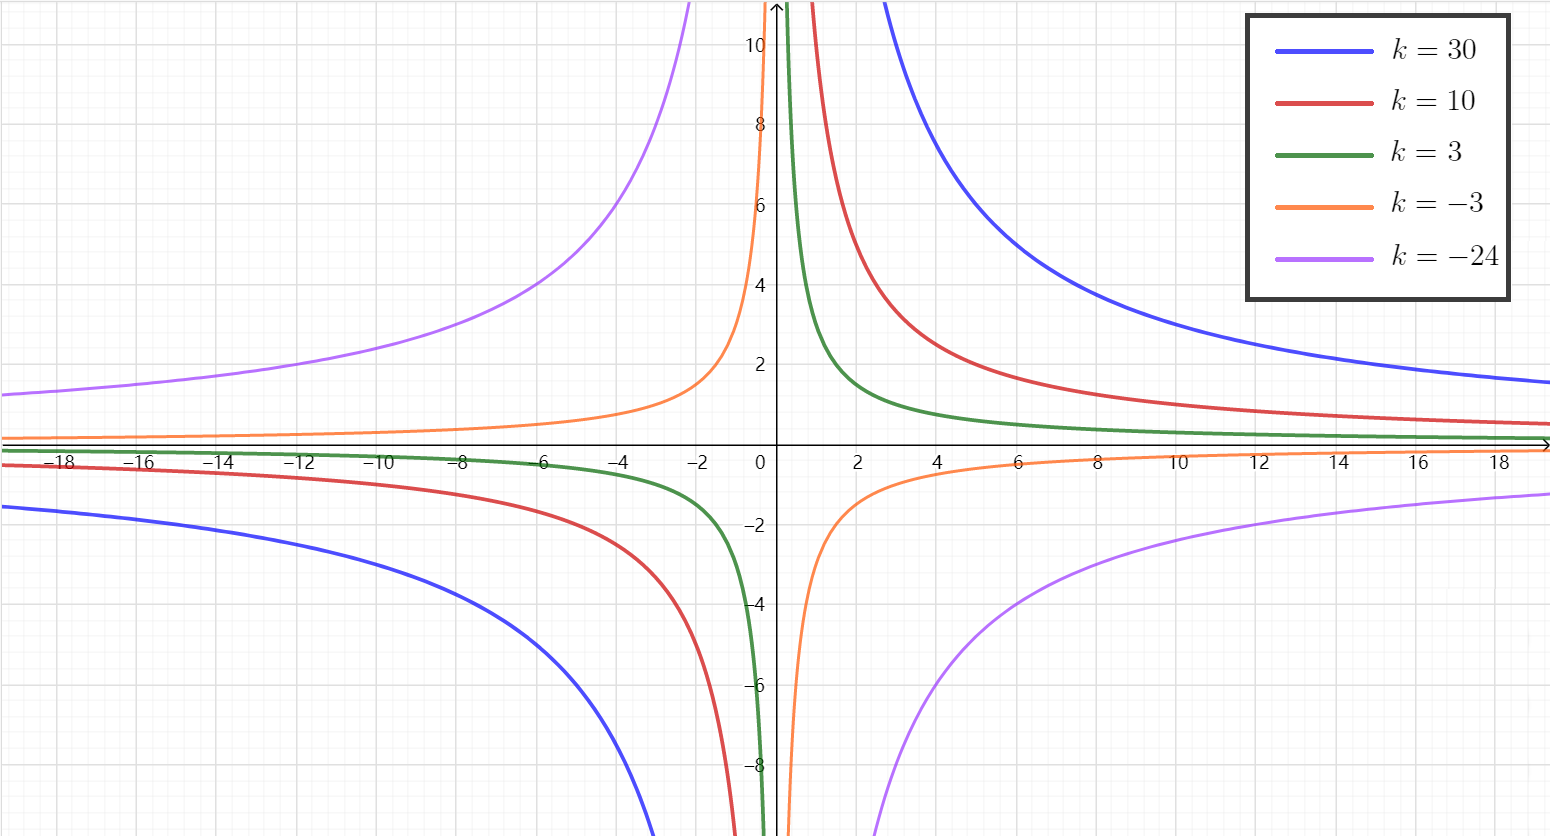
\includegraphics[width=0.9\textwidth]{tu/反比例函数2.png}
\end{figure}

首先，$k=3$的图像和$k=-3$的函数图像恰好关于$y$轴对称，也关于$x$轴对称。
一般来说，$k<0$时，函数图像和$-k$时的函数图像关于$y$轴和$x$轴对称。
由对称性，我们可以只研究$k>0$情况下函数图像的正支。

对比上图第一象限中三种颜色的曲线，我们可以发现，每条曲线都随着$x$变大而越来越平缓，
$x$越靠近$0$，曲线就越陡峭。观察不同曲线之间的区别，可以发现，$k$越大，曲线越“靠右上方”。
这并不难理解。比如，对横坐标$x = 4$来说，正数$k$越大，纵坐标$\frac{k}{4}$就越大，在图像中越“靠上”。
同样，要让纵坐标$f(x) = 4$，那么对应的横坐标$x = \frac{k}{4}$，于是正数$k$越大，$\frac{k}{4}$就越大，
在图像中越“靠右”。

反比例函数的图像还有一个基本性质：如果点$(a, \,\,b)$在图像上，那么$(b, \,\,a)$也在图像上。
这是因为$a = \frac{k}{b}$，当且仅当$b = \frac{k}{a}$。
\begin{xt}\label{xt:5-0-0}
    证明：\\
    \indent 1. 只要$(a, \,\,b)$在函数$x \mapsto \frac{k}{x}$的图像上，那么$(b, \,\,a)$、$(-a, \,\,-b)$、$(-b, \,\,-a)$
    都在图像上。\\
    \indent 2. 如果斜率为$-1$的直线$x\mapsto -x + c$和函数$ x \mapsto \frac{k}{x}$的图像有交点，
    那么$c^2 \geqslant 4k$。
\end{xt}

\section{二次函数}
一元一次式对应一次函数，而一元二次式对应着二次函数。一般来说，一元二次式可以写成$ax^2 + bx + c$的形式，
其中$a \neq 0$。我们把形如
$$ x \mapsto ax^2 + bx + c$$
的函数叫做二次函数。

我们从最简单的情形：$x\mapsto x^2$开始研究。下表是$x$取不同值时函数的值：

\begin{center}
    \begin{tabular}{| p{2em}<{\centering} | p{1.8em}<{\centering} | p{1.8em}<{\centering} | p{1.8em}<{\centering} | p{1.8em}<{\centering} | p{1.8em}<{\centering} | p{1.8em}<{\centering} | p{1.8em}<{\centering} | p{1.8em}<{\centering} | p{1.8em}<{\centering} |}
        \hline
        $x$ & -10 & -5 & -2 & -1 & 0 & 1 & 2 & 5 & 10 \\ [0.5ex] 
        \hline
        $f(x)$ & 100 & 25 & 4 & 1 & 0 & 1 & 4 & 25 & 100 \\   
        \hline
    \end{tabular}
\end{center}

首先可以发现，如果$a$和$b$是相反数，那么$f(a) = f(b)$。比如，$f(-5) = f(5)$、$f(-2) = f(2)$、
$f(-1) = f(1)$。这个性质可以写成：
$$ f(-x) = f(x).$$
这个性质可以用函数的定义证明：
$$ f(-x) = (-x)^2 = x^2 = f(x).$$

另外可以看到，$x<0$时，$f(x)$大于$0$，且$x$越大，$f(x)$越小，最终在$x=0$时函数值取$0$。
$x > 0$是，$f(x)$大于$0$，且$x$越大，$f(x)$越大。

函数$x\mapsto x^2$的图像是怎样的呢？和反比例函数情形一样：我们可以用描点法得到大致的模样，但目前我们掌握的知识，
还不足以严谨地勾画出它的图像。借助计算机作图软件，我们可以得到函数$x\mapsto x^2$的图像：

\begin{figure}[h] %this figure will be at the right
    \vspace{8pt}
    \centering
    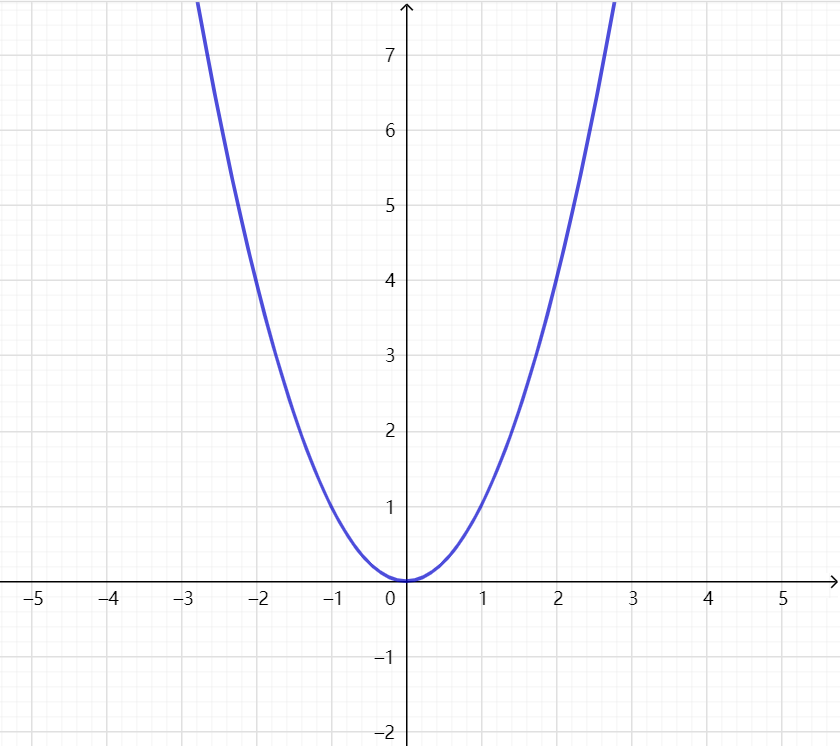
\includegraphics[width=0.6\textwidth]{tu/二次函数1.png}
\end{figure}

观察图像，这是一条曲线。首先可以注意到，它关于$y$轴对称。这一点可以用前面得到的性质证明。给定图像上一点：
$(x, \,\,x^2)$，$(-x, \,\,x^2)$也在图像上，所以图像关于$y$轴对称。由对称性，
我们可以先研究曲线在$x\geqslant 0$部分的性质。

可以发现，从$x=0$开始，随着$x$逐渐增大，函数值也逐渐增大，而且增长速度逐渐加快。
在$x=0$附近，曲线比较平缓，$x$增大后，曲线越来越陡峭。

如果把函数乘以系数$a$，得到$x\mapsto ax^2$，函数的性质会发生什么变化？
我们可以验证：$a > 0$时，以上提到的性质保持不变。$a < 0$时，函数的正负和增减性质颠倒了。
首先，$ax^2$总小于等于$0$。$x<0$时，$x$越大，函数值越大，$x>0$时，$x$越大，函数值越小。
从$x=0$开始，随着$x$逐渐增大，函数值逐渐减小，而且减小速度逐渐加快。
与$a>0$时相同的是：在$x=0$附近，曲线比较平缓，$x$增大后，曲线越来越陡峭。

\begin{figure}[h] %this figure will be at the right
    \vspace{8pt}
    \centering
    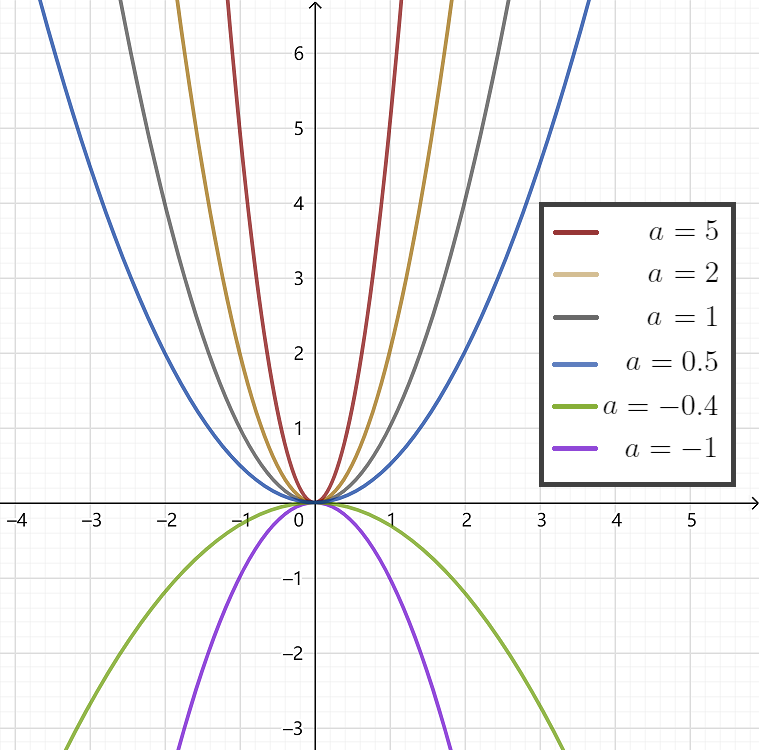
\includegraphics[width=0.5\textwidth]{tu/二次函数2.png}
\end{figure}

对于一般的一元二次式$ax^2+bx+c$，二次函数$x\mapsto ax^2+bx+c$的图像是怎样的呢？
上一章中，我们使用配方法解一元二次方程。用同样的方法，我们可以把$ax^2+bx+c$
写成：
\begin{align*}
    ax^2+bx+c &= a\left(x + \frac{b}{2a}\right)^2 + \frac{4ac - b^2}{4a}  \\
    &= a\left(x + \frac{b}{2a}\right)^2 - \frac{\Delta}{4a}. 
\end{align*}

因此，如果我们把$x\mapsto ax^2$的图像按$\left(-\frac{b}{2a}, \,\,-\frac{\Delta}{4a}\right)$平移，
就得到$x\mapsto ax^2+bx+c$的图像。
比如，要得到$x\mapsto 0.5x^2+0.8x-1$的图像，我们从
$x\mapsto 0.5x^2$出发。将$0.5x^2+0.8x-1$配方得到
$$ 0.5x^2+0.8x-1 = 0.5\left(x + 0.8\right)^2 - 1.32$$
于是将$x\mapsto 0.5x^2$按$(-0.8, \,\,-1.32)$平移，就得到$x\mapsto 0.5x^2+0.8x-1$的图像。

\begin{figure}[ht] %this figure will be at the right
    \centering
    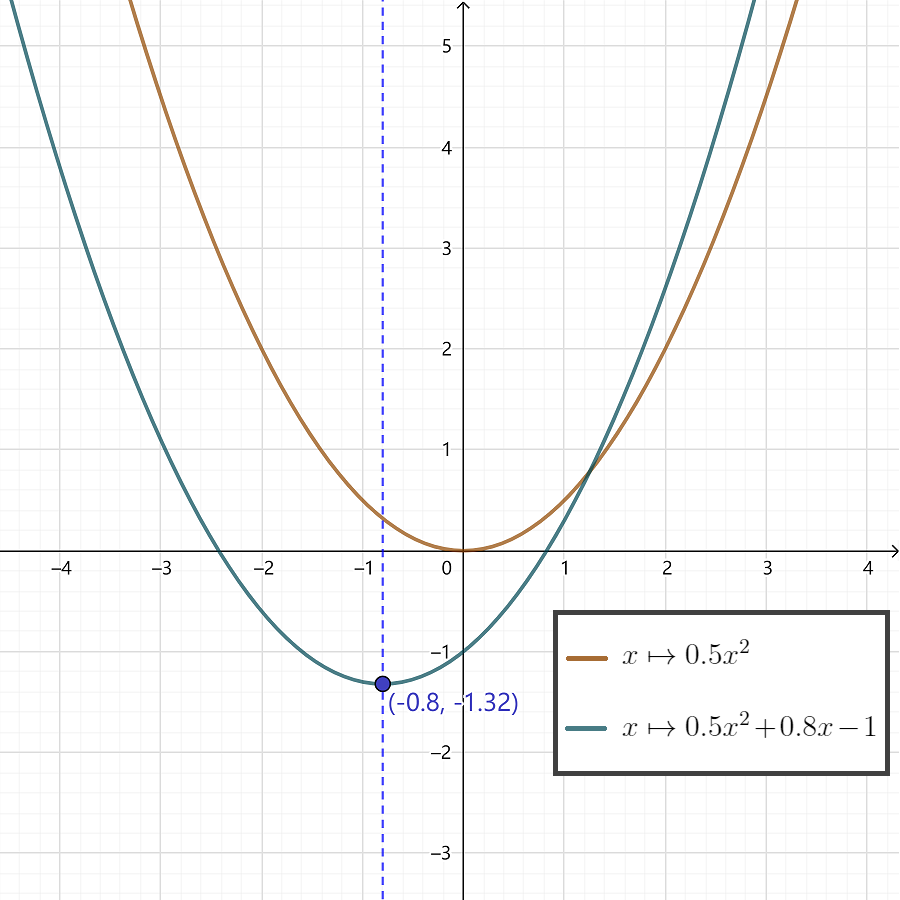
\includegraphics[width=0.45\textwidth]{tu/二次函数3.png}
\end{figure}

用$x\mapsto 0.5x^2+0.8x-1$作例子，可以看到，原来$x\mapsto ax^2$的图像关于$y$轴对称。
平移之后，图像关于直线$x = -\frac{b}{2a}$对称。$a>0$时，$x\mapsto ax^2$的图像最低点是$(0,\,\,0)$，
平移之后，最低点是$\left(-\frac{b}{2a}, \,\,-\frac{\Delta}{4a}\right)$。
$a<0$时，$x\mapsto ax^2$的图像最高点是$(0,\,\,0)$，
平移之后，最高点是$\left(-\frac{b}{2a}, \,\,-\frac{\Delta}{4a}\right)$。
直线$x = -\frac{b}{2a}$叫做二次函数图像的对称轴，
点$\left(-\frac{b}{2a}, \,\,-\frac{\Delta}{4a}\right)$叫做\textbf{二次函数图像的顶点}。
\begin{xt}\label{xt:5-1-0}
    \mbox{} \\    
    \indent 1. 二次函数$x\mapsto x^2$的图像和$x\mapsto ax + b$恰有一个交点，
    那么$a$、$b$满足怎样的关系？交点的坐标是多少？\\
    \indent 2. 二次函数$x\mapsto ax^2+bx+c$的图像和它关于点$(x_0, y_0)$平移后的图像有交点，
    则$(x_0, y_0)$应满足什么条件？交点个数可以是多少？
\end{xt}

\section{一元二次不等式}
通过研究二次函数的图像，我们可以直观地理解一元二次不等式。

一元二次不等式是类似$ax^2 + bx + c > 0$的不等式。其中的大于号也可以是小于号、大于等于号或小于等于号。
以不等式$ax^2 + bx + c > 0$来说，$x$是不等式的一个解，当且仅当点$(x, ax^2 + bx + c)$在$x$轴上方。
也就是说，$ax^2 + bx + c > 0$的解集，就是二次函数$ x \mapsto ax^2 + bx + c$在$x$轴上方的点的横坐标的集合。

观察$x \mapsto ax^2 + bx + c$的图像可知，如果$\Delta>0$，那么二次函数有两个零点。
$a>0$时，不等式的解集对应两个零点两侧的部分，是两个开区间的并集：
$$ (-\infty; \frac{-b - \Delta}{2a}) \cup (\frac{-b +\Delta}{2a}; \infty)$$
$a<0$时，不等式的解集对应两个零点之间的部分，即开区间：
$$ (\frac{-b - \Delta}{2a}; \frac{-b +\Delta}{2a}) $$
如果$\Delta<0$，那么二次函数没有零点。$a>0$时，二次函数的图像总在$x$轴上方，于是不等式的解集是全体实数。
$a<0$时，二次函数的图像总在$x$轴下方，于是不等式的解集是空集。

如果$\Delta = 0$，那么二次函数恰有一个零点。
$a>0$时，不等式的解集对应零点两侧的部分，是两个开区间的并集：
$$ (-\infty; \frac{-b}{2a}) \cup (\frac{-b}{2a}; \infty)$$
$a<0$时，二次函数的值不大于零，于是不等式的解集是空集。

要是不等式的大于号换成大于等于号，则相关的“开”的部分也换成“闭”。如果$\Delta>0$，二次函数有两个零点。
$a>0$时，不等式$ax^2 + bx + c \geqslant 0$的解集是：
$$ (-\infty; \frac{-b - \Delta}{2a}\,] \cup [\,\frac{-b +\Delta}{2a}; \infty)$$
$a<0$时，不等式的解集是：
$$ [\,\frac{-b - \Delta}{2a}; \frac{-b +\Delta}{2a}\,] $$
如果$\Delta<0$，那么二次函数没有零点。$a>0$时，二次函数的图像总在$x$轴上方，于是不等式的解集是全体实数。
$a<0$时，二次函数的图像总在$x$轴下方，于是不等式的解集是空集。

如果$\Delta = 0$，那么二次函数恰有一个零点。
$a>0$时，不等式的解集包括了零点，因此是全体实数。
$a<0$时，二次函数的值不大于零，于是不等式的解集是单元集：$\{\frac{-b}{2a}\}$。

要是不等式的大于号（大于等于号）换成小于号（小于等于号），只需要把左边的项移到右边，
就转化成大于号（大于等于号）的情况。

\begin{ex}
    \mbox{}\\
    \indent 1. 求不等式$2x^2 - 5x + 2 > 0$的解集。\\
    \indent 2. 求不等式$x^2 - 6x + 9 \geqslant 0$的解集。
\end{ex}
\begin{so}
    \mbox{}\\
    \indent 1. 首先求一元二次方程$2x^2 - 5x + 2 = 0$的解。依公式可得：
    $$ x_1 = 0.5, \quad x_2 = 2.$$
    因此，不等式的解集是$(-\infty; 0.5) \cup (2; \infty)$。\\
    \indent 2. 首先求一元二次方程$x^2 - 6x + 9 = 0$的解。依公式可得：
    $$ x = 3.$$
    因此，不等式的解集是全体实数。
\end{so}

一元二次不等式还可以用来解反比例函数和一次函数的不等式。
\begin{ex}
    求不等式$\frac{8}{x} > x + 2$的解集。
\end{ex}
可以把这个不等式理解为反比例函数$x \mapsto \frac{8}{x}$和一次函数$x \mapsto x + 2$的图像的关系。
$x$是不等式$\frac{8}{x} > x + 2$的一个解，当且仅当点$(x, \frac{8}{x})$在点$(x, \,\,x + 2)$上方。
如果我们画出两个函数的图像，并找到反比例函数在$x \mapsto \frac{8}{x}$在一次函数$x \mapsto x + 2$
图像上方的部分，那么这部分的点的横坐标，就是不等式的解。

观察两者图像可知，解集大致对应第三象限中曲线和直线交点左侧的部分，以及第一象限中曲线和直线交点左侧的部分。
具体交点的位置，我们可以通过解方程$\frac{8}{x} = x + 2$得到。而这个方程可以转化为一元二次方程。

\begin{figure}[h]
    \vspace{4pt}
    \centering
    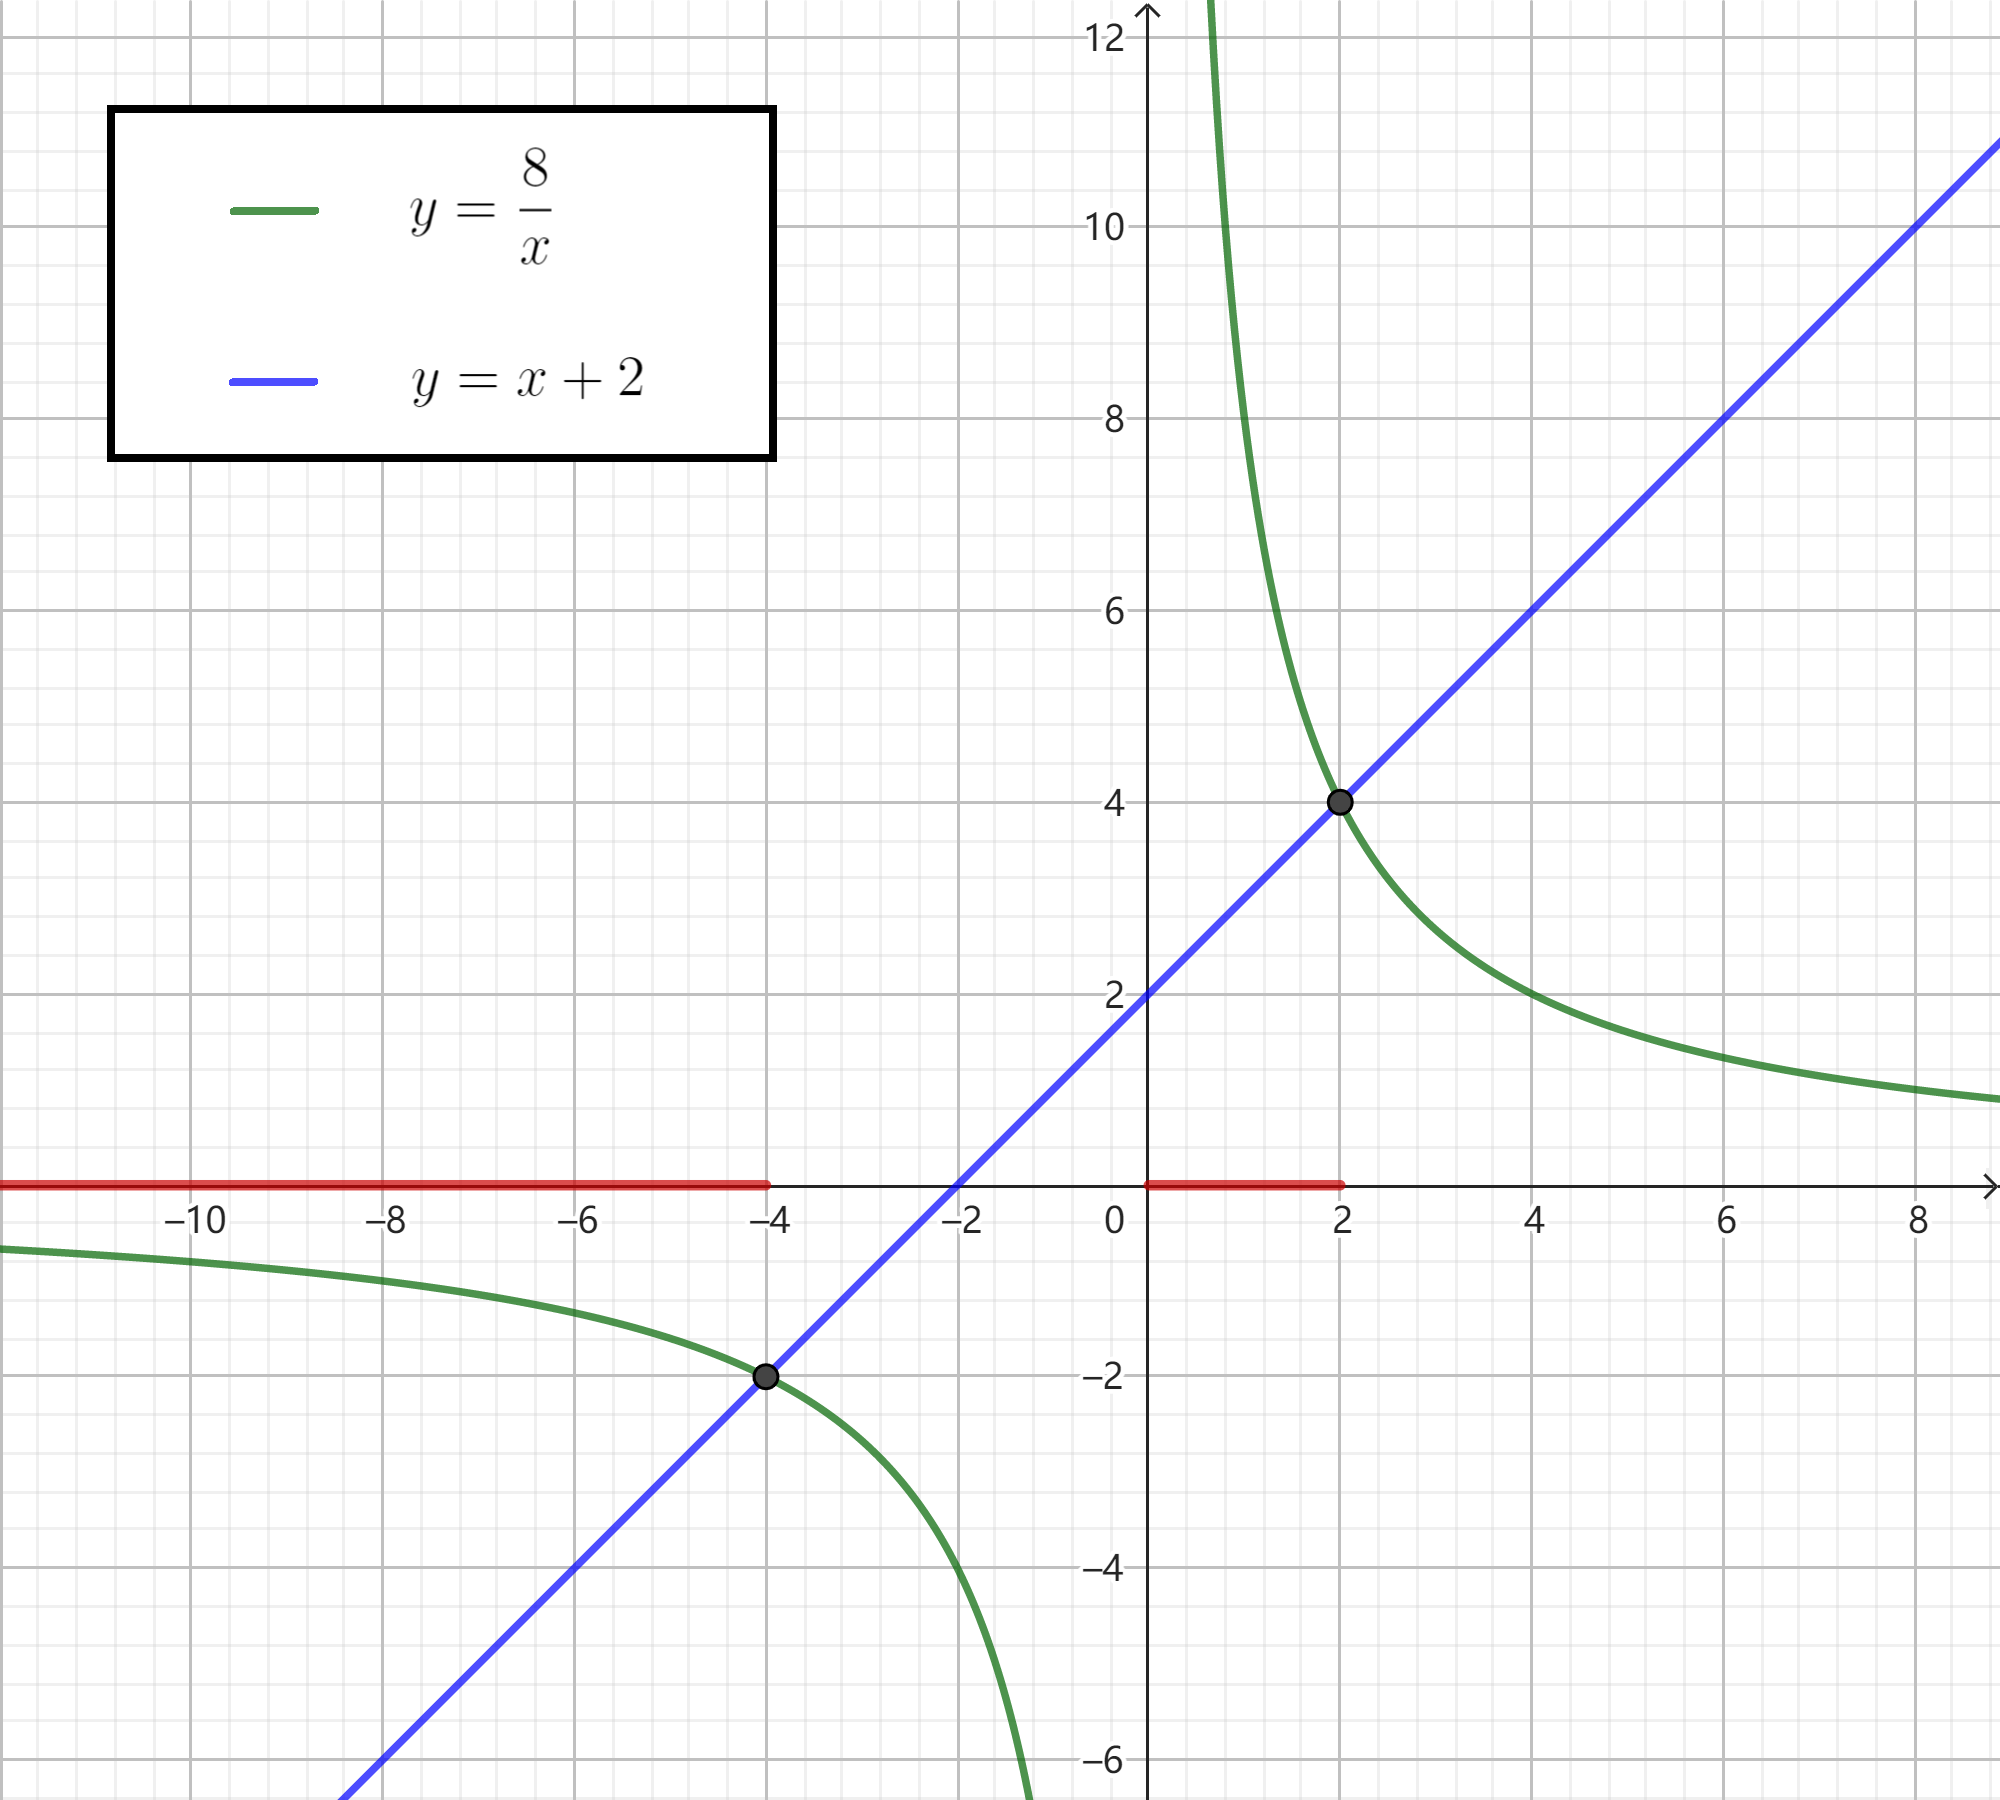
\includegraphics[width=0.5\textwidth]{tu/一元二次不等式1.png}
\end{figure}

把$\frac{8}{x} = x + 2$两边乘以$x$，再把常数项$8$移到右边，就得到方程：
$$ 0 =  x^2 + 2x - 8.$$
这是一个一元二次方程，解为：
$$ x_1 = -4, \quad x_2 = 2$$
它们分别对应点$(-4, \,\,-2)$和$(2, \,\,4)$（注意不是$(-4, \,\,0)$和$(2, \,\,0)$）。这两个点就是第三、第一象限中曲线和直线交点的位置。
因此，我们可以得出结论：不等式的解集是$(-\infty; -4) \cup (0; 2)$。

\begin{xt}\label{xt:5-2-0}
    解以下不等式：\\
    \indent 1. $3x^2 - 8x + 4 < 0$ \\
    \indent 2. $2x^2 + 8x + 9 \geqslant 7x + 10$ \\
    \indent 3. $\frac{2}{x} < 6x- 7$ 
\end{xt}

\begin{appendix}

\chapter{常用对数表}

常用对数表是用来指明$a = 10^b$中$a$和$b$的关系的。$10$称为常用对数表的底数。$a$和$b$分别称为真数和对数。

常用对数表以$0.001$的间隔，给出了查询从$1.001$到$9.999$一共$9999$个真数的对数的方法。每个真数有四位数字，我们把个位数字和小数点后第一位数字合称为\textbf{首数}。比如$2.718$的首数是“$2.7$”。在表中找到$2.7$对应的行。行中有$19$列。左侧的$10$列是小数点后第二位数字对应的\textbf{基数}，右侧的$9$列是根据小数点后第三位数字“$8$”的\textbf{比例调整数}。基数与比例调整数之和就是对数的小数部分。如果真数小数点后第三位是$0$，则不需要调整，基数就是对数的小数部分。

举例来说，想要查询$2.718$的对数，就在表中找到“$2.7$”对应的行。在左侧$10$列中找到数字“$1$”对应的列（左起第$2$列）。这一列的数值是“$4330$”。然后在右侧$9$列中找到数字“$8$”对应的列（右起第$2$列），这一列的数值是“$13$”。于是$2.718$的对数的小数部分是两者的和：$4330 + 13 = 4343$。也就是说，$2.718$的对数是$0.4343$。如果查询的是$2.71$的对数，那么无需调整，对数就是$0.4330$。

反之，已知$0$到$1$之间的对数，可以借助对数表反查真数。在对数表的左侧$10$列（基数部分）从上到下，从左往右逐个寻找比对数的小数点后四位数字小的最大基数。要注意的是，每一行基数从左到右越来越大，每一行最右边的数小于下一行最左边的数，可以按此规律查找。找到符合条件的基数后，要么完全吻合，于是真数就是对应的首数后添上对应列的列号。如果不完全吻合，那么从基数开始，分别加上该行右侧$9$列的比例调整数，看哪个与对数最接近。这时，对数的真数就是对应的首数后添上对应列的列号，再添上调整数的列号。

举例来说，要查找$0.5136$对应的真数，就在表格左侧$10$列基数里找比$5136$小的最大基数。结果是“$3.2$”行的第$7$列：$5132$。于是真数介于$3.26$和$3.27$之间。再给$5132$分别加上“$3.2$”行右侧的比例调整数：$5133$、$5135$、$5136$、$5137$，……发现第$3$列恰好是我们要找的$5136$。因此$0.5136$对应的真数是$3.263$。如果要查找的是$0.5132$，它对应的真数就是$3.26$，无需再查看比例调整数。

\vspace{8pt}

\setlength{\tabcolsep}{2pt} % 调整列间距
\begin{longtable}{|c| c c c c c | c c c c c| c c c c c c c c c|}
\caption*{\textbf{常用对数表}} \\
\toprule
\multirow{2}{*}{首数} & \multirow{2}{*}{0} & \multirow{2}{*}{1} & \multirow{2}{*}{2} & \multirow{2}{*}{3} & \multirow{2}{*}{4} & \multirow{2}{*}{5} & \multirow{2}{*}{6} & \multirow{2}{*}{7} & \multirow{2}{*}{8} & \multirow{2}{*}{9} & \multicolumn{9}{c}{\phantom{啊w}比例调整数\phantom{啊w}} \\
\cline{12-20}
 &  &  &  &  &  &  &  &  &  &  & 1 & 2 & 3 & 4 & 5 & 6 & 7 & 8 & 9 \\
\midrule
\endfirsthead

\toprule
\multirow{2}{*}{首数} & \multirow{2}{*}{0} & \multirow{2}{*}{1} & \multirow{2}{*}{2} & \multirow{2}{*}{3} & \multirow{2}{*}{4} & \multirow{2}{*}{5} & \multirow{2}{*}{6} & \multirow{2}{*}{7} & \multirow{2}{*}{8} & \multirow{2}{*}{9} & \multicolumn{9}{c}{\phantom{啊w}比例调整数\phantom{啊w}} \\
\cline{12-20}
 &  &  &  &  &  &  &  &  &  &  & 1 & 2 & 3 & 4 & 5 & 6 & 7 & 8 & 9 \\
\midrule
\endhead
\scriptsize 1.0 & \scriptsize 0000 & \scriptsize 0043 & \scriptsize 0086 & \scriptsize 0128 & \scriptsize 0170 & \scriptsize 0212 & \scriptsize 0253 & \scriptsize 0294 & \scriptsize 0334 & \scriptsize 0374 & \scriptsize 04 & \scriptsize 08 & \scriptsize 12 & \scriptsize 17 & \scriptsize 21 & \scriptsize 25 & \scriptsize 29 & \scriptsize 33 & \scriptsize 37 \\
\scriptsize 1.1 & \scriptsize 0414 & \scriptsize 0453 & \scriptsize 0492 & \scriptsize 0531 & \scriptsize 0569 & \scriptsize 0607 & \scriptsize 0645 & \scriptsize 0682 & \scriptsize 0719 & \scriptsize 0755 & \scriptsize 04 & \scriptsize 08 & \scriptsize 11 & \scriptsize 15 & \scriptsize 19 & \scriptsize 23 & \scriptsize 26 & \scriptsize 30 & \scriptsize 34 \\
\scriptsize 1.2 & \scriptsize 0792 & \scriptsize 0828 & \scriptsize 0864 & \scriptsize 0899 & \scriptsize 0934 & \scriptsize 0969 & \scriptsize 1004 & \scriptsize 1038 & \scriptsize 1072 & \scriptsize 1106 & \scriptsize 03 & \scriptsize 07 & \scriptsize 10 & \scriptsize 14 & \scriptsize 17 & \scriptsize 21 & \scriptsize 24 & \scriptsize 28 & \scriptsize 31 \\
\scriptsize 1.3 & \scriptsize 1139 & \scriptsize 1173 & \scriptsize 1206 & \scriptsize 1239 & \scriptsize 1271 & \scriptsize 1303 & \scriptsize 1335 & \scriptsize 1367 & \scriptsize 1399 & \scriptsize 1430 & \scriptsize 03 & \scriptsize 06 & \scriptsize 10 & \scriptsize 13 & \scriptsize 16 & \scriptsize 19 & \scriptsize 23 & \scriptsize 26 & \scriptsize 29 \\
\scriptsize 1.4 & \scriptsize 1461 & \scriptsize 1492 & \scriptsize 1523 & \scriptsize 1553 & \scriptsize 1584 & \scriptsize 1614 & \scriptsize 1644 & \scriptsize 1673 & \scriptsize 1703 & \scriptsize 1732 & \scriptsize 03 & \scriptsize 06 & \scriptsize 09 & \scriptsize 12 & \scriptsize 15 & \scriptsize 18 & \scriptsize 21 & \scriptsize 24 & \scriptsize 27 \\
\scriptsize 1.5 & \scriptsize 1761 & \scriptsize 1790 & \scriptsize 1818 & \scriptsize 1847 & \scriptsize 1875 & \scriptsize 1903 & \scriptsize 1931 & \scriptsize 1959 & \scriptsize 1987 & \scriptsize 2014 & \scriptsize 03 & \scriptsize 06 & \scriptsize 08 & \scriptsize 11 & \scriptsize 14 & \scriptsize 17 & \scriptsize 20 & \scriptsize 22 & \scriptsize 25 \\
\scriptsize 1.6 & \scriptsize 2041 & \scriptsize 2068 & \scriptsize 2095 & \scriptsize 2122 & \scriptsize 2148 & \scriptsize 2175 & \scriptsize 2201 & \scriptsize 2227 & \scriptsize 2253 & \scriptsize 2279 & \scriptsize 03 & \scriptsize 05 & \scriptsize 08 & \scriptsize 11 & \scriptsize 13 & \scriptsize 16 & \scriptsize 18 & \scriptsize 21 & \scriptsize 24 \\
\scriptsize 1.7 & \scriptsize 2304 & \scriptsize 2330 & \scriptsize 2355 & \scriptsize 2380 & \scriptsize 2405 & \scriptsize 2430 & \scriptsize 2455 & \scriptsize 2480 & \scriptsize 2504 & \scriptsize 2529 & \scriptsize 02 & \scriptsize 05 & \scriptsize 07 & \scriptsize 10 & \scriptsize 12 & \scriptsize 15 & \scriptsize 17 & \scriptsize 20 & \scriptsize 22 \\
\scriptsize 1.8 & \scriptsize 2553 & \scriptsize 2577 & \scriptsize 2601 & \scriptsize 2625 & \scriptsize 2648 & \scriptsize 2672 & \scriptsize 2695 & \scriptsize 2718 & \scriptsize 2742 & \scriptsize 2765 & \scriptsize 02 & \scriptsize 05 & \scriptsize 07 & \scriptsize 09 & \scriptsize 12 & \scriptsize 14 & \scriptsize 16 & \scriptsize 19 & \scriptsize 21 \\
\scriptsize 1.9 & \scriptsize 2788 & \scriptsize 2810 & \scriptsize 2833 & \scriptsize 2856 & \scriptsize 2878 & \scriptsize 2900 & \scriptsize 2923 & \scriptsize 2945 & \scriptsize 2967 & \scriptsize 2989 & \scriptsize 02 & \scriptsize 04 & \scriptsize 07 & \scriptsize 09 & \scriptsize 11 & \scriptsize 13 & \scriptsize 16 & \scriptsize 18 & \scriptsize 20 \\
\scriptsize 2.0 & \scriptsize 3010 & \scriptsize 3032 & \scriptsize 3054 & \scriptsize 3075 & \scriptsize 3096 & \scriptsize 3118 & \scriptsize 3139 & \scriptsize 3160 & \scriptsize 3181 & \scriptsize 3201 & \scriptsize 02 & \scriptsize 04 & \scriptsize 06 & \scriptsize 08 & \scriptsize 11 & \scriptsize 13 & \scriptsize 15 & \scriptsize 17 & \scriptsize 19 \\
\scriptsize 2.1 & \scriptsize 3222 & \scriptsize 3243 & \scriptsize 3263 & \scriptsize 3284 & \scriptsize 3304 & \scriptsize 3324 & \scriptsize 3345 & \scriptsize 3365 & \scriptsize 3385 & \scriptsize 3404 & \scriptsize 02 & \scriptsize 04 & \scriptsize 06 & \scriptsize 08 & \scriptsize 10 & \scriptsize 12 & \scriptsize 14 & \scriptsize 16 & \scriptsize 18 \\
\scriptsize 2.2 & \scriptsize 3424 & \scriptsize 3444 & \scriptsize 3464 & \scriptsize 3483 & \scriptsize 3502 & \scriptsize 3522 & \scriptsize 3541 & \scriptsize 3560 & \scriptsize 3579 & \scriptsize 3598 & \scriptsize 02 & \scriptsize 04 & \scriptsize 06 & \scriptsize 08 & \scriptsize 10 & \scriptsize 12 & \scriptsize 14 & \scriptsize 15 & \scriptsize 17 \\
\scriptsize 2.3 & \scriptsize 3617 & \scriptsize 3636 & \scriptsize 3655 & \scriptsize 3674 & \scriptsize 3692 & \scriptsize 3711 & \scriptsize 3729 & \scriptsize 3747 & \scriptsize 3766 & \scriptsize 3784 & \scriptsize 02 & \scriptsize 04 & \scriptsize 06 & \scriptsize 07 & \scriptsize 09 & \scriptsize 11 & \scriptsize 13 & \scriptsize 15 & \scriptsize 17 \\
\scriptsize 2.4 & \scriptsize 3802 & \scriptsize 3820 & \scriptsize 3838 & \scriptsize 3856 & \scriptsize 3874 & \scriptsize 3892 & \scriptsize 3909 & \scriptsize 3927 & \scriptsize 3945 & \scriptsize 3962 & \scriptsize 02 & \scriptsize 04 & \scriptsize 05 & \scriptsize 07 & \scriptsize 09 & \scriptsize 11 & \scriptsize 12 & \scriptsize 14 & \scriptsize 16 \\
\scriptsize 2.5 & \scriptsize 3979 & \scriptsize 3997 & \scriptsize 4014 & \scriptsize 4031 & \scriptsize 4048 & \scriptsize 4065 & \scriptsize 4082 & \scriptsize 4099 & \scriptsize 4116 & \scriptsize 4133 & \scriptsize 02 & \scriptsize 03 & \scriptsize 05 & \scriptsize 07 & \scriptsize 09 & \scriptsize 10 & \scriptsize 12 & \scriptsize 14 & \scriptsize 15 \\
\scriptsize 2.6 & \scriptsize 4150 & \scriptsize 4166 & \scriptsize 4183 & \scriptsize 4200 & \scriptsize 4216 & \scriptsize 4232 & \scriptsize 4249 & \scriptsize 4265 & \scriptsize 4281 & \scriptsize 4298 & \scriptsize 02 & \scriptsize 03 & \scriptsize 05 & \scriptsize 07 & \scriptsize 08 & \scriptsize 10 & \scriptsize 11 & \scriptsize 13 & \scriptsize 15 \\
\scriptsize 2.7 & \scriptsize 4314 & \scriptsize 4330 & \scriptsize 4346 & \scriptsize 4362 & \scriptsize 4378 & \scriptsize 4393 & \scriptsize 4409 & \scriptsize 4425 & \scriptsize 4440 & \scriptsize 4456 & \scriptsize 02 & \scriptsize 03 & \scriptsize 05 & \scriptsize 06 & \scriptsize 08 & \scriptsize 09 & \scriptsize 11 & \scriptsize 13 & \scriptsize 14 \\
\scriptsize 2.8 & \scriptsize 4472 & \scriptsize 4487 & \scriptsize 4502 & \scriptsize 4518 & \scriptsize 4533 & \scriptsize 4548 & \scriptsize 4564 & \scriptsize 4579 & \scriptsize 4594 & \scriptsize 4609 & \scriptsize 02 & \scriptsize 03 & \scriptsize 05 & \scriptsize 06 & \scriptsize 08 & \scriptsize 09 & \scriptsize 11 & \scriptsize 12 & \scriptsize 14 \\
\scriptsize 2.9 & \scriptsize 4624 & \scriptsize 4639 & \scriptsize 4654 & \scriptsize 4669 & \scriptsize 4683 & \scriptsize 4698 & \scriptsize 4713 & \scriptsize 4728 & \scriptsize 4742 & \scriptsize 4757 & \scriptsize 01 & \scriptsize 03 & \scriptsize 04 & \scriptsize 06 & \scriptsize 07 & \scriptsize 09 & \scriptsize 10 & \scriptsize 12 & \scriptsize 13 \\
\scriptsize 3.0 & \scriptsize 4771 & \scriptsize 4786 & \scriptsize 4800 & \scriptsize 4814 & \scriptsize 4829 & \scriptsize 4843 & \scriptsize 4857 & \scriptsize 4871 & \scriptsize 4886 & \scriptsize 4900 & \scriptsize 01 & \scriptsize 03 & \scriptsize 04 & \scriptsize 06 & \scriptsize 07 & \scriptsize 09 & \scriptsize 10 & \scriptsize 11 & \scriptsize 13 \\
\scriptsize 3.1 & \scriptsize 4914 & \scriptsize 4928 & \scriptsize 4942 & \scriptsize 4955 & \scriptsize 4969 & \scriptsize 4983 & \scriptsize 4997 & \scriptsize 5011 & \scriptsize 5024 & \scriptsize 5038 & \scriptsize 01 & \scriptsize 03 & \scriptsize 04 & \scriptsize 06 & \scriptsize 07 & \scriptsize 08 & \scriptsize 10 & \scriptsize 11 & \scriptsize 12 \\
\scriptsize 3.2 & \scriptsize 5051 & \scriptsize 5065 & \scriptsize 5079 & \scriptsize 5092 & \scriptsize 5105 & \scriptsize 5119 & \scriptsize 5132 & \scriptsize 5145 & \scriptsize 5159 & \scriptsize 5172 & \scriptsize 01 & \scriptsize 03 & \scriptsize 04 & \scriptsize 05 & \scriptsize 07 & \scriptsize 08 & \scriptsize 09 & \scriptsize 11 & \scriptsize 12 \\
\scriptsize 3.3 & \scriptsize 5185 & \scriptsize 5198 & \scriptsize 5211 & \scriptsize 5224 & \scriptsize 5237 & \scriptsize 5250 & \scriptsize 5263 & \scriptsize 5276 & \scriptsize 5289 & \scriptsize 5302 & \scriptsize 01 & \scriptsize 03 & \scriptsize 04 & \scriptsize 05 & \scriptsize 06 & \scriptsize 08 & \scriptsize 09 & \scriptsize 10 & \scriptsize 12 \\
\scriptsize 3.4 & \scriptsize 5315 & \scriptsize 5328 & \scriptsize 5340 & \scriptsize 5353 & \scriptsize 5366 & \scriptsize 5378 & \scriptsize 5391 & \scriptsize 5403 & \scriptsize 5416 & \scriptsize 5428 & \scriptsize 01 & \scriptsize 03 & \scriptsize 04 & \scriptsize 05 & \scriptsize 06 & \scriptsize 08 & \scriptsize 09 & \scriptsize 10 & \scriptsize 11 \\
\scriptsize 3.5 & \scriptsize 5441 & \scriptsize 5453 & \scriptsize 5465 & \scriptsize 5478 & \scriptsize 5490 & \scriptsize 5502 & \scriptsize 5514 & \scriptsize 5527 & \scriptsize 5539 & \scriptsize 5551 & \scriptsize 01 & \scriptsize 02 & \scriptsize 04 & \scriptsize 05 & \scriptsize 06 & \scriptsize 07 & \scriptsize 09 & \scriptsize 10 & \scriptsize 11 \\
\scriptsize 3.6 & \scriptsize 5563 & \scriptsize 5575 & \scriptsize 5587 & \scriptsize 5599 & \scriptsize 5611 & \scriptsize 5623 & \scriptsize 5635 & \scriptsize 5647 & \scriptsize 5658 & \scriptsize 5670 & \scriptsize 01 & \scriptsize 02 & \scriptsize 04 & \scriptsize 05 & \scriptsize 06 & \scriptsize 07 & \scriptsize 08 & \scriptsize 10 & \scriptsize 11 \\
\scriptsize 3.7 & \scriptsize 5682 & \scriptsize 5694 & \scriptsize 5705 & \scriptsize 5717 & \scriptsize 5729 & \scriptsize 5740 & \scriptsize 5752 & \scriptsize 5763 & \scriptsize 5775 & \scriptsize 5786 & \scriptsize 01 & \scriptsize 02 & \scriptsize 03 & \scriptsize 05 & \scriptsize 06 & \scriptsize 07 & \scriptsize 08 & \scriptsize 09 & \scriptsize 10 \\
\scriptsize 3.8 & \scriptsize 5798 & \scriptsize 5809 & \scriptsize 5821 & \scriptsize 5832 & \scriptsize 5843 & \scriptsize 5855 & \scriptsize 5866 & \scriptsize 5877 & \scriptsize 5888 & \scriptsize 5899 & \scriptsize 01 & \scriptsize 02 & \scriptsize 03 & \scriptsize 05 & \scriptsize 06 & \scriptsize 07 & \scriptsize 08 & \scriptsize 09 & \scriptsize 10 \\
\scriptsize 3.9 & \scriptsize 5911 & \scriptsize 5922 & \scriptsize 5933 & \scriptsize 5944 & \scriptsize 5955 & \scriptsize 5966 & \scriptsize 5977 & \scriptsize 5988 & \scriptsize 5999 & \scriptsize 6010 & \scriptsize 01 & \scriptsize 02 & \scriptsize 03 & \scriptsize 04 & \scriptsize 06 & \scriptsize 07 & \scriptsize 08 & \scriptsize 09 & \scriptsize 10 \\
\scriptsize 4.0 & \scriptsize 6021 & \scriptsize 6031 & \scriptsize 6042 & \scriptsize 6053 & \scriptsize 6064 & \scriptsize 6075 & \scriptsize 6085 & \scriptsize 6096 & \scriptsize 6107 & \scriptsize 6117 & \scriptsize 01 & \scriptsize 02 & \scriptsize 03 & \scriptsize 04 & \scriptsize 05 & \scriptsize 06 & \scriptsize 08 & \scriptsize 09 & \scriptsize 10 \\
\scriptsize 4.1 & \scriptsize 6128 & \scriptsize 6138 & \scriptsize 6149 & \scriptsize 6160 & \scriptsize 6170 & \scriptsize 6180 & \scriptsize 6191 & \scriptsize 6201 & \scriptsize 6212 & \scriptsize 6222 & \scriptsize 01 & \scriptsize 02 & \scriptsize 03 & \scriptsize 04 & \scriptsize 05 & \scriptsize 06 & \scriptsize 07 & \scriptsize 08 & \scriptsize 09 \\
\scriptsize 4.2 & \scriptsize 6232 & \scriptsize 6243 & \scriptsize 6253 & \scriptsize 6263 & \scriptsize 6274 & \scriptsize 6284 & \scriptsize 6294 & \scriptsize 6304 & \scriptsize 6314 & \scriptsize 6325 & \scriptsize 01 & \scriptsize 02 & \scriptsize 03 & \scriptsize 04 & \scriptsize 05 & \scriptsize 06 & \scriptsize 07 & \scriptsize 08 & \scriptsize 09 \\
\scriptsize 4.3 & \scriptsize 6335 & \scriptsize 6345 & \scriptsize 6355 & \scriptsize 6365 & \scriptsize 6375 & \scriptsize 6385 & \scriptsize 6395 & \scriptsize 6405 & \scriptsize 6415 & \scriptsize 6425 & \scriptsize 01 & \scriptsize 02 & \scriptsize 03 & \scriptsize 04 & \scriptsize 05 & \scriptsize 06 & \scriptsize 07 & \scriptsize 08 & \scriptsize 09 \\
\scriptsize 4.4 & \scriptsize 6435 & \scriptsize 6444 & \scriptsize 6454 & \scriptsize 6464 & \scriptsize 6474 & \scriptsize 6484 & \scriptsize 6493 & \scriptsize 6503 & \scriptsize 6513 & \scriptsize 6522 & \scriptsize 01 & \scriptsize 02 & \scriptsize 03 & \scriptsize 04 & \scriptsize 05 & \scriptsize 06 & \scriptsize 07 & \scriptsize 08 & \scriptsize 09 \\
\scriptsize 4.5 & \scriptsize 6532 & \scriptsize 6542 & \scriptsize 6551 & \scriptsize 6561 & \scriptsize 6571 & \scriptsize 6580 & \scriptsize 6590 & \scriptsize 6599 & \scriptsize 6609 & \scriptsize 6618 & \scriptsize 01 & \scriptsize 02 & \scriptsize 03 & \scriptsize 04 & \scriptsize 05 & \scriptsize 06 & \scriptsize 07 & \scriptsize 08 & \scriptsize 09 \\
\scriptsize 4.6 & \scriptsize 6628 & \scriptsize 6637 & \scriptsize 6646 & \scriptsize 6656 & \scriptsize 6665 & \scriptsize 6675 & \scriptsize 6684 & \scriptsize 6693 & \scriptsize 6702 & \scriptsize 6712 & \scriptsize 01 & \scriptsize 02 & \scriptsize 03 & \scriptsize 04 & \scriptsize 05 & \scriptsize 06 & \scriptsize 07 & \scriptsize 07 & \scriptsize 08 \\
\scriptsize 4.7 & \scriptsize 6721 & \scriptsize 6730 & \scriptsize 6739 & \scriptsize 6749 & \scriptsize 6758 & \scriptsize 6767 & \scriptsize 6776 & \scriptsize 6785 & \scriptsize 6794 & \scriptsize 6803 & \scriptsize 01 & \scriptsize 02 & \scriptsize 03 & \scriptsize 04 & \scriptsize 05 & \scriptsize 05 & \scriptsize 06 & \scriptsize 07 & \scriptsize 08 \\
\scriptsize 4.8 & \scriptsize 6812 & \scriptsize 6821 & \scriptsize 6830 & \scriptsize 6839 & \scriptsize 6848 & \scriptsize 6857 & \scriptsize 6866 & \scriptsize 6875 & \scriptsize 6884 & \scriptsize 6893 & \scriptsize 01 & \scriptsize 02 & \scriptsize 03 & \scriptsize 04 & \scriptsize 04 & \scriptsize 05 & \scriptsize 06 & \scriptsize 07 & \scriptsize 08 \\
\scriptsize 4.9 & \scriptsize 6902 & \scriptsize 6911 & \scriptsize 6920 & \scriptsize 6928 & \scriptsize 6937 & \scriptsize 6946 & \scriptsize 6955 & \scriptsize 6964 & \scriptsize 6972 & \scriptsize 6981 & \scriptsize 01 & \scriptsize 02 & \scriptsize 03 & \scriptsize 04 & \scriptsize 04 & \scriptsize 05 & \scriptsize 06 & \scriptsize 07 & \scriptsize 08 \\
\scriptsize 5.0 & \scriptsize 6990 & \scriptsize 6998 & \scriptsize 7007 & \scriptsize 7016 & \scriptsize 7024 & \scriptsize 7033 & \scriptsize 7042 & \scriptsize 7050 & \scriptsize 7059 & \scriptsize 7067 & \scriptsize 01 & \scriptsize 02 & \scriptsize 03 & \scriptsize 03 & \scriptsize 04 & \scriptsize 05 & \scriptsize 06 & \scriptsize 07 & \scriptsize 08 \\
\scriptsize 5.1 & \scriptsize 7076 & \scriptsize 7084 & \scriptsize 7093 & \scriptsize 7101 & \scriptsize 7110 & \scriptsize 7118 & \scriptsize 7126 & \scriptsize 7135 & \scriptsize 7143 & \scriptsize 7152 & \scriptsize 01 & \scriptsize 02 & \scriptsize 03 & \scriptsize 03 & \scriptsize 04 & \scriptsize 05 & \scriptsize 06 & \scriptsize 07 & \scriptsize 08 \\
\scriptsize 5.2 & \scriptsize 7160 & \scriptsize 7168 & \scriptsize 7177 & \scriptsize 7185 & \scriptsize 7193 & \scriptsize 7202 & \scriptsize 7210 & \scriptsize 7218 & \scriptsize 7226 & \scriptsize 7235 & \scriptsize 01 & \scriptsize 02 & \scriptsize 02 & \scriptsize 03 & \scriptsize 04 & \scriptsize 05 & \scriptsize 06 & \scriptsize 07 & \scriptsize 07 \\
\scriptsize 5.3 & \scriptsize 7243 & \scriptsize 7251 & \scriptsize 7259 & \scriptsize 7267 & \scriptsize 7275 & \scriptsize 7284 & \scriptsize 7292 & \scriptsize 7300 & \scriptsize 7308 & \scriptsize 7316 & \scriptsize 01 & \scriptsize 02 & \scriptsize 02 & \scriptsize 03 & \scriptsize 04 & \scriptsize 05 & \scriptsize 06 & \scriptsize 06 & \scriptsize 07 \\
\scriptsize 5.4 & \scriptsize 7324 & \scriptsize 7332 & \scriptsize 7340 & \scriptsize 7348 & \scriptsize 7356 & \scriptsize 7364 & \scriptsize 7372 & \scriptsize 7380 & \scriptsize 7388 & \scriptsize 7396 & \scriptsize 01 & \scriptsize 02 & \scriptsize 02 & \scriptsize 03 & \scriptsize 04 & \scriptsize 05 & \scriptsize 06 & \scriptsize 06 & \scriptsize 07 \\
\scriptsize 5.5 & \scriptsize 7404 & \scriptsize 7412 & \scriptsize 7419 & \scriptsize 7427 & \scriptsize 7435 & \scriptsize 7443 & \scriptsize 7451 & \scriptsize 7459 & \scriptsize 7466 & \scriptsize 7474 & \scriptsize 01 & \scriptsize 02 & \scriptsize 02 & \scriptsize 03 & \scriptsize 04 & \scriptsize 05 & \scriptsize 05 & \scriptsize 06 & \scriptsize 07 \\
\scriptsize 5.6 & \scriptsize 7482 & \scriptsize 7490 & \scriptsize 7497 & \scriptsize 7505 & \scriptsize 7513 & \scriptsize 7520 & \scriptsize 7528 & \scriptsize 7536 & \scriptsize 7543 & \scriptsize 7551 & \scriptsize 01 & \scriptsize 02 & \scriptsize 02 & \scriptsize 03 & \scriptsize 04 & \scriptsize 05 & \scriptsize 05 & \scriptsize 06 & \scriptsize 07 \\
\scriptsize 5.7 & \scriptsize 7559 & \scriptsize 7566 & \scriptsize 7574 & \scriptsize 7582 & \scriptsize 7589 & \scriptsize 7597 & \scriptsize 7604 & \scriptsize 7612 & \scriptsize 7619 & \scriptsize 7627 & \scriptsize 01 & \scriptsize 02 & \scriptsize 02 & \scriptsize 03 & \scriptsize 04 & \scriptsize 05 & \scriptsize 05 & \scriptsize 06 & \scriptsize 07 \\
\scriptsize 5.8 & \scriptsize 7634 & \scriptsize 7642 & \scriptsize 7649 & \scriptsize 7657 & \scriptsize 7664 & \scriptsize 7672 & \scriptsize 7679 & \scriptsize 7686 & \scriptsize 7694 & \scriptsize 7701 & \scriptsize 01 & \scriptsize 01 & \scriptsize 02 & \scriptsize 03 & \scriptsize 04 & \scriptsize 04 & \scriptsize 05 & \scriptsize 06 & \scriptsize 07 \\
\scriptsize 5.9 & \scriptsize 7709 & \scriptsize 7716 & \scriptsize 7723 & \scriptsize 7731 & \scriptsize 7738 & \scriptsize 7745 & \scriptsize 7752 & \scriptsize 7760 & \scriptsize 7767 & \scriptsize 7774 & \scriptsize 01 & \scriptsize 01 & \scriptsize 02 & \scriptsize 03 & \scriptsize 04 & \scriptsize 04 & \scriptsize 05 & \scriptsize 06 & \scriptsize 07 \\
\scriptsize 6.0 & \scriptsize 7782 & \scriptsize 7789 & \scriptsize 7796 & \scriptsize 7803 & \scriptsize 7810 & \scriptsize 7818 & \scriptsize 7825 & \scriptsize 7832 & \scriptsize 7839 & \scriptsize 7846 & \scriptsize 01 & \scriptsize 01 & \scriptsize 02 & \scriptsize 03 & \scriptsize 04 & \scriptsize 04 & \scriptsize 05 & \scriptsize 06 & \scriptsize 06 \\
\scriptsize 6.1 & \scriptsize 7853 & \scriptsize 7860 & \scriptsize 7868 & \scriptsize 7875 & \scriptsize 7882 & \scriptsize 7889 & \scriptsize 7896 & \scriptsize 7903 & \scriptsize 7910 & \scriptsize 7917 & \scriptsize 01 & \scriptsize 01 & \scriptsize 02 & \scriptsize 03 & \scriptsize 04 & \scriptsize 04 & \scriptsize 05 & \scriptsize 06 & \scriptsize 06 \\
\scriptsize 6.2 & \scriptsize 7924 & \scriptsize 7931 & \scriptsize 7938 & \scriptsize 7945 & \scriptsize 7952 & \scriptsize 7959 & \scriptsize 7966 & \scriptsize 7973 & \scriptsize 7980 & \scriptsize 7987 & \scriptsize 01 & \scriptsize 01 & \scriptsize 02 & \scriptsize 03 & \scriptsize 03 & \scriptsize 04 & \scriptsize 05 & \scriptsize 06 & \scriptsize 06 \\
\scriptsize 6.3 & \scriptsize 7993 & \scriptsize 8000 & \scriptsize 8007 & \scriptsize 8014 & \scriptsize 8021 & \scriptsize 8028 & \scriptsize 8035 & \scriptsize 8041 & \scriptsize 8048 & \scriptsize 8055 & \scriptsize 01 & \scriptsize 01 & \scriptsize 02 & \scriptsize 03 & \scriptsize 03 & \scriptsize 04 & \scriptsize 05 & \scriptsize 05 & \scriptsize 06 \\
\scriptsize 6.4 & \scriptsize 8062 & \scriptsize 8069 & \scriptsize 8075 & \scriptsize 8082 & \scriptsize 8089 & \scriptsize 8096 & \scriptsize 8102 & \scriptsize 8109 & \scriptsize 8116 & \scriptsize 8122 & \scriptsize 01 & \scriptsize 01 & \scriptsize 02 & \scriptsize 03 & \scriptsize 03 & \scriptsize 04 & \scriptsize 05 & \scriptsize 05 & \scriptsize 06 \\
\scriptsize 6.5 & \scriptsize 8129 & \scriptsize 8136 & \scriptsize 8142 & \scriptsize 8149 & \scriptsize 8156 & \scriptsize 8162 & \scriptsize 8169 & \scriptsize 8176 & \scriptsize 8182 & \scriptsize 8189 & \scriptsize 01 & \scriptsize 01 & \scriptsize 02 & \scriptsize 03 & \scriptsize 03 & \scriptsize 04 & \scriptsize 05 & \scriptsize 05 & \scriptsize 06 \\
\scriptsize 6.6 & \scriptsize 8195 & \scriptsize 8202 & \scriptsize 8209 & \scriptsize 8215 & \scriptsize 8222 & \scriptsize 8228 & \scriptsize 8235 & \scriptsize 8241 & \scriptsize 8248 & \scriptsize 8254 & \scriptsize 01 & \scriptsize 01 & \scriptsize 02 & \scriptsize 03 & \scriptsize 03 & \scriptsize 04 & \scriptsize 05 & \scriptsize 05 & \scriptsize 06 \\
\scriptsize 6.7 & \scriptsize 8261 & \scriptsize 8267 & \scriptsize 8274 & \scriptsize 8280 & \scriptsize 8287 & \scriptsize 8293 & \scriptsize 8299 & \scriptsize 8306 & \scriptsize 8312 & \scriptsize 8319 & \scriptsize 01 & \scriptsize 01 & \scriptsize 02 & \scriptsize 03 & \scriptsize 03 & \scriptsize 04 & \scriptsize 05 & \scriptsize 05 & \scriptsize 06 \\
\scriptsize 6.8 & \scriptsize 8325 & \scriptsize 8331 & \scriptsize 8338 & \scriptsize 8344 & \scriptsize 8351 & \scriptsize 8357 & \scriptsize 8363 & \scriptsize 8370 & \scriptsize 8376 & \scriptsize 8382 & \scriptsize 01 & \scriptsize 01 & \scriptsize 02 & \scriptsize 03 & \scriptsize 03 & \scriptsize 04 & \scriptsize 04 & \scriptsize 05 & \scriptsize 06 \\
\scriptsize 6.9 & \scriptsize 8388 & \scriptsize 8395 & \scriptsize 8401 & \scriptsize 8407 & \scriptsize 8414 & \scriptsize 8420 & \scriptsize 8426 & \scriptsize 8432 & \scriptsize 8439 & \scriptsize 8445 & \scriptsize 01 & \scriptsize 01 & \scriptsize 02 & \scriptsize 03 & \scriptsize 03 & \scriptsize 04 & \scriptsize 04 & \scriptsize 05 & \scriptsize 06 \\
\scriptsize 7.0 & \scriptsize 8451 & \scriptsize 8457 & \scriptsize 8463 & \scriptsize 8470 & \scriptsize 8476 & \scriptsize 8482 & \scriptsize 8488 & \scriptsize 8494 & \scriptsize 8500 & \scriptsize 8506 & \scriptsize 01 & \scriptsize 01 & \scriptsize 02 & \scriptsize 02 & \scriptsize 03 & \scriptsize 04 & \scriptsize 04 & \scriptsize 05 & \scriptsize 06 \\
\scriptsize 7.1 & \scriptsize 8513 & \scriptsize 8519 & \scriptsize 8525 & \scriptsize 8531 & \scriptsize 8537 & \scriptsize 8543 & \scriptsize 8549 & \scriptsize 8555 & \scriptsize 8561 & \scriptsize 8567 & \scriptsize 01 & \scriptsize 01 & \scriptsize 02 & \scriptsize 02 & \scriptsize 03 & \scriptsize 04 & \scriptsize 04 & \scriptsize 05 & \scriptsize 05 \\
\scriptsize 7.2 & \scriptsize 8573 & \scriptsize 8579 & \scriptsize 8585 & \scriptsize 8591 & \scriptsize 8597 & \scriptsize 8603 & \scriptsize 8609 & \scriptsize 8615 & \scriptsize 8621 & \scriptsize 8627 & \scriptsize 01 & \scriptsize 01 & \scriptsize 02 & \scriptsize 02 & \scriptsize 03 & \scriptsize 04 & \scriptsize 04 & \scriptsize 05 & \scriptsize 05 \\
\scriptsize 7.3 & \scriptsize 8633 & \scriptsize 8639 & \scriptsize 8645 & \scriptsize 8651 & \scriptsize 8657 & \scriptsize 8663 & \scriptsize 8669 & \scriptsize 8675 & \scriptsize 8681 & \scriptsize 8686 & \scriptsize 01 & \scriptsize 01 & \scriptsize 02 & \scriptsize 02 & \scriptsize 03 & \scriptsize 04 & \scriptsize 04 & \scriptsize 05 & \scriptsize 05 \\
\scriptsize 7.4 & \scriptsize 8692 & \scriptsize 8698 & \scriptsize 8704 & \scriptsize 8710 & \scriptsize 8716 & \scriptsize 8722 & \scriptsize 8727 & \scriptsize 8733 & \scriptsize 8739 & \scriptsize 8745 & \scriptsize 01 & \scriptsize 01 & \scriptsize 02 & \scriptsize 02 & \scriptsize 03 & \scriptsize 03 & \scriptsize 04 & \scriptsize 05 & \scriptsize 05 \\
\scriptsize 7.5 & \scriptsize 8751 & \scriptsize 8756 & \scriptsize 8762 & \scriptsize 8768 & \scriptsize 8774 & \scriptsize 8779 & \scriptsize 8785 & \scriptsize 8791 & \scriptsize 8797 & \scriptsize 8802 & \scriptsize 01 & \scriptsize 01 & \scriptsize 02 & \scriptsize 02 & \scriptsize 03 & \scriptsize 03 & \scriptsize 04 & \scriptsize 05 & \scriptsize 05 \\
\scriptsize 7.6 & \scriptsize 8808 & \scriptsize 8814 & \scriptsize 8820 & \scriptsize 8825 & \scriptsize 8831 & \scriptsize 8837 & \scriptsize 8842 & \scriptsize 8848 & \scriptsize 8854 & \scriptsize 8859 & \scriptsize 01 & \scriptsize 01 & \scriptsize 02 & \scriptsize 02 & \scriptsize 03 & \scriptsize 03 & \scriptsize 04 & \scriptsize 05 & \scriptsize 05 \\
\scriptsize 7.7 & \scriptsize 8865 & \scriptsize 8871 & \scriptsize 8876 & \scriptsize 8882 & \scriptsize 8887 & \scriptsize 8893 & \scriptsize 8899 & \scriptsize 8904 & \scriptsize 8910 & \scriptsize 8915 & \scriptsize 01 & \scriptsize 01 & \scriptsize 02 & \scriptsize 02 & \scriptsize 03 & \scriptsize 03 & \scriptsize 04 & \scriptsize 04 & \scriptsize 05 \\
\scriptsize 7.8 & \scriptsize 8921 & \scriptsize 8927 & \scriptsize 8932 & \scriptsize 8938 & \scriptsize 8943 & \scriptsize 8949 & \scriptsize 8954 & \scriptsize 8960 & \scriptsize 8965 & \scriptsize 8971 & \scriptsize 01 & \scriptsize 01 & \scriptsize 02 & \scriptsize 02 & \scriptsize 03 & \scriptsize 03 & \scriptsize 04 & \scriptsize 04 & \scriptsize 05 \\
\scriptsize 7.9 & \scriptsize 8976 & \scriptsize 8982 & \scriptsize 8987 & \scriptsize 8993 & \scriptsize 8998 & \scriptsize 9004 & \scriptsize 9009 & \scriptsize 9015 & \scriptsize 9020 & \scriptsize 9025 & \scriptsize 01 & \scriptsize 01 & \scriptsize 02 & \scriptsize 02 & \scriptsize 03 & \scriptsize 03 & \scriptsize 04 & \scriptsize 04 & \scriptsize 05 \\
\scriptsize 8.0 & \scriptsize 9031 & \scriptsize 9036 & \scriptsize 9042 & \scriptsize 9047 & \scriptsize 9053 & \scriptsize 9058 & \scriptsize 9063 & \scriptsize 9069 & \scriptsize 9074 & \scriptsize 9079 & \scriptsize 01 & \scriptsize 01 & \scriptsize 02 & \scriptsize 02 & \scriptsize 03 & \scriptsize 03 & \scriptsize 04 & \scriptsize 04 & \scriptsize 05 \\
\scriptsize 8.1 & \scriptsize 9085 & \scriptsize 9090 & \scriptsize 9096 & \scriptsize 9101 & \scriptsize 9106 & \scriptsize 9112 & \scriptsize 9117 & \scriptsize 9122 & \scriptsize 9128 & \scriptsize 9133 & \scriptsize 01 & \scriptsize 01 & \scriptsize 02 & \scriptsize 02 & \scriptsize 03 & \scriptsize 03 & \scriptsize 04 & \scriptsize 04 & \scriptsize 05 \\
\scriptsize 8.2 & \scriptsize 9138 & \scriptsize 9143 & \scriptsize 9149 & \scriptsize 9154 & \scriptsize 9159 & \scriptsize 9165 & \scriptsize 9170 & \scriptsize 9175 & \scriptsize 9180 & \scriptsize 9186 & \scriptsize 01 & \scriptsize 01 & \scriptsize 02 & \scriptsize 02 & \scriptsize 03 & \scriptsize 03 & \scriptsize 04 & \scriptsize 04 & \scriptsize 05 \\
\scriptsize 8.3 & \scriptsize 9191 & \scriptsize 9196 & \scriptsize 9201 & \scriptsize 9206 & \scriptsize 9212 & \scriptsize 9217 & \scriptsize 9222 & \scriptsize 9227 & \scriptsize 9232 & \scriptsize 9238 & \scriptsize 01 & \scriptsize 01 & \scriptsize 02 & \scriptsize 02 & \scriptsize 03 & \scriptsize 03 & \scriptsize 04 & \scriptsize 04 & \scriptsize 05 \\
\scriptsize 8.4 & \scriptsize 9243 & \scriptsize 9248 & \scriptsize 9253 & \scriptsize 9258 & \scriptsize 9263 & \scriptsize 9269 & \scriptsize 9274 & \scriptsize 9279 & \scriptsize 9284 & \scriptsize 9289 & \scriptsize 01 & \scriptsize 01 & \scriptsize 02 & \scriptsize 02 & \scriptsize 03 & \scriptsize 03 & \scriptsize 04 & \scriptsize 04 & \scriptsize 05 \\
\scriptsize 8.5 & \scriptsize 9294 & \scriptsize 9299 & \scriptsize 9304 & \scriptsize 9309 & \scriptsize 9315 & \scriptsize 9320 & \scriptsize 9325 & \scriptsize 9330 & \scriptsize 9335 & \scriptsize 9340 & \scriptsize 01 & \scriptsize 01 & \scriptsize 02 & \scriptsize 02 & \scriptsize 03 & \scriptsize 03 & \scriptsize 04 & \scriptsize 04 & \scriptsize 05 \\
\scriptsize 8.6 & \scriptsize 9345 & \scriptsize 9350 & \scriptsize 9355 & \scriptsize 9360 & \scriptsize 9365 & \scriptsize 9370 & \scriptsize 9375 & \scriptsize 9380 & \scriptsize 9385 & \scriptsize 9390 & \scriptsize 01 & \scriptsize 01 & \scriptsize 02 & \scriptsize 02 & \scriptsize 03 & \scriptsize 03 & \scriptsize 04 & \scriptsize 04 & \scriptsize 05 \\
\scriptsize 8.7 & \scriptsize 9395 & \scriptsize 9400 & \scriptsize 9405 & \scriptsize 9410 & \scriptsize 9415 & \scriptsize 9420 & \scriptsize 9425 & \scriptsize 9430 & \scriptsize 9435 & \scriptsize 9440 & \scriptsize 00 & \scriptsize 01 & \scriptsize 01 & \scriptsize 02 & \scriptsize 02 & \scriptsize 03 & \scriptsize 03 & \scriptsize 04 & \scriptsize 04 \\
\scriptsize 8.8 & \scriptsize 9445 & \scriptsize 9450 & \scriptsize 9455 & \scriptsize 9460 & \scriptsize 9465 & \scriptsize 9469 & \scriptsize 9474 & \scriptsize 9479 & \scriptsize 9484 & \scriptsize 9489 & \scriptsize 00 & \scriptsize 01 & \scriptsize 01 & \scriptsize 02 & \scriptsize 02 & \scriptsize 03 & \scriptsize 03 & \scriptsize 04 & \scriptsize 04 \\
\scriptsize 8.9 & \scriptsize 9494 & \scriptsize 9499 & \scriptsize 9504 & \scriptsize 9509 & \scriptsize 9513 & \scriptsize 9518 & \scriptsize 9523 & \scriptsize 9528 & \scriptsize 9533 & \scriptsize 9538 & \scriptsize 00 & \scriptsize 01 & \scriptsize 01 & \scriptsize 02 & \scriptsize 02 & \scriptsize 03 & \scriptsize 03 & \scriptsize 04 & \scriptsize 04 \\
\scriptsize 9.0 & \scriptsize 9542 & \scriptsize 9547 & \scriptsize 9552 & \scriptsize 9557 & \scriptsize 9562 & \scriptsize 9566 & \scriptsize 9571 & \scriptsize 9576 & \scriptsize 9581 & \scriptsize 9586 & \scriptsize 00 & \scriptsize 01 & \scriptsize 01 & \scriptsize 02 & \scriptsize 02 & \scriptsize 03 & \scriptsize 03 & \scriptsize 04 & \scriptsize 04 \\
\scriptsize 9.1 & \scriptsize 9590 & \scriptsize 9595 & \scriptsize 9600 & \scriptsize 9605 & \scriptsize 9609 & \scriptsize 9614 & \scriptsize 9619 & \scriptsize 9624 & \scriptsize 9628 & \scriptsize 9633 & \scriptsize 00 & \scriptsize 01 & \scriptsize 01 & \scriptsize 02 & \scriptsize 02 & \scriptsize 03 & \scriptsize 03 & \scriptsize 04 & \scriptsize 04 \\
\scriptsize 9.2 & \scriptsize 9638 & \scriptsize 9643 & \scriptsize 9647 & \scriptsize 9652 & \scriptsize 9657 & \scriptsize 9661 & \scriptsize 9666 & \scriptsize 9671 & \scriptsize 9675 & \scriptsize 9680 & \scriptsize 00 & \scriptsize 01 & \scriptsize 01 & \scriptsize 02 & \scriptsize 02 & \scriptsize 03 & \scriptsize 03 & \scriptsize 04 & \scriptsize 04 \\
\scriptsize 9.3 & \scriptsize 9685 & \scriptsize 9689 & \scriptsize 9694 & \scriptsize 9699 & \scriptsize 9703 & \scriptsize 9708 & \scriptsize 9713 & \scriptsize 9717 & \scriptsize 9722 & \scriptsize 9727 & \scriptsize 00 & \scriptsize 01 & \scriptsize 01 & \scriptsize 02 & \scriptsize 02 & \scriptsize 03 & \scriptsize 03 & \scriptsize 04 & \scriptsize 04 \\
\scriptsize 9.4 & \scriptsize 9731 & \scriptsize 9736 & \scriptsize 9741 & \scriptsize 9745 & \scriptsize 9750 & \scriptsize 9754 & \scriptsize 9759 & \scriptsize 9763 & \scriptsize 9768 & \scriptsize 9773 & \scriptsize 00 & \scriptsize 01 & \scriptsize 01 & \scriptsize 02 & \scriptsize 02 & \scriptsize 03 & \scriptsize 03 & \scriptsize 04 & \scriptsize 04 \\
\scriptsize 9.5 & \scriptsize 9777 & \scriptsize 9782 & \scriptsize 9786 & \scriptsize 9791 & \scriptsize 9795 & \scriptsize 9800 & \scriptsize 9805 & \scriptsize 9809 & \scriptsize 9814 & \scriptsize 9818 & \scriptsize 00 & \scriptsize 01 & \scriptsize 01 & \scriptsize 02 & \scriptsize 02 & \scriptsize 03 & \scriptsize 03 & \scriptsize 04 & \scriptsize 04 \\
\scriptsize 9.6 & \scriptsize 9823 & \scriptsize 9827 & \scriptsize 9832 & \scriptsize 9836 & \scriptsize 9841 & \scriptsize 9845 & \scriptsize 9850 & \scriptsize 9854 & \scriptsize 9859 & \scriptsize 9863 & \scriptsize 00 & \scriptsize 01 & \scriptsize 01 & \scriptsize 02 & \scriptsize 02 & \scriptsize 03 & \scriptsize 03 & \scriptsize 04 & \scriptsize 04 \\
\scriptsize 9.7 & \scriptsize 9868 & \scriptsize 9872 & \scriptsize 9877 & \scriptsize 9881 & \scriptsize 9886 & \scriptsize 9890 & \scriptsize 9894 & \scriptsize 9899 & \scriptsize 9903 & \scriptsize 9908 & \scriptsize 00 & \scriptsize 01 & \scriptsize 01 & \scriptsize 02 & \scriptsize 02 & \scriptsize 03 & \scriptsize 03 & \scriptsize 04 & \scriptsize 04 \\
\scriptsize 9.8 & \scriptsize 9912 & \scriptsize 9917 & \scriptsize 9921 & \scriptsize 9926 & \scriptsize 9930 & \scriptsize 9934 & \scriptsize 9939 & \scriptsize 9943 & \scriptsize 9948 & \scriptsize 9952 & \scriptsize 00 & \scriptsize 01 & \scriptsize 01 & \scriptsize 02 & \scriptsize 02 & \scriptsize 03 & \scriptsize 03 & \scriptsize 04 & \scriptsize 04 \\
\scriptsize 9.9 & \scriptsize 9956 & \scriptsize 9961 & \scriptsize 9965 & \scriptsize 9969 & \scriptsize 9974 & \scriptsize 9978 & \scriptsize 9983 & \scriptsize 9987 & \scriptsize 9991 & \scriptsize 9996 & \scriptsize 00 & \scriptsize 01 & \scriptsize 01 & \scriptsize 02 & \scriptsize 02 & \scriptsize 03 & \scriptsize 03 & \scriptsize 03 & \scriptsize 04 \\
\hline
\end{longtable}


\end{appendix}




\end{document}